% FEUP THESIS STYLE for LaTeX2e
% how to use feupteses (changed from the original for MIEEC)
%
% FEUP, JCL & JCF, Tue May 20 18:53:15 2008
%
% PLEASE send improvements to jlopes at fe.up.pt, jcf at fe.up.pt
%

%%========================================
%% Commands: pdflatex mieic
%%           bibtex mieic
%%           makeindex mieic (only if crating an index) 
%%           pdflatex mieic
%%========================================

%% For one side layout comment next line and uncomment the second line
\documentclass[11pt,a4paper,twoside,openright]{report}
\usepackage[utf8]{inputenx}
\usepackage[official]{eurosym}
\usepackage[english]{babel}
\usepackage{amsmath}
\usepackage{amsfonts}
\usepackage{tkz-graph}
\usepackage{multirow}
\usepackage{longtable} % needs font/line height hack (it's local right now)

\usepackage{verbatim}
\makeatletter 
\g@addto@macro\@verbatim\small 
\makeatother 

\usepackage{color}
\definecolor{grey}{rgb}{0.53,0.53,0.53}
\definecolor{red}{rgb}{0.87,0.13,0.0}
\definecolor{green}{rgb}{0.0,0.53,0.0}

\usepackage{listings}
\lstset{
language=Ruby,                   % choose the language of the code
basicstyle=\footnotesize,       % the size of the fonts that are used for the code
backgroundcolor=\color{white},  % choose the background color. You must add \usepackage{color}
showspaces=false,               % show spaces adding particular underscores
showstringspaces=false,         % underline spaces within strings
showtabs=false,                 % show tabs within strings adding particular underscores
frame=single,	                  % adds a frame around the code
tabsize=2,	                    % sets default tabsize to 4 spaces
captionpos=t,                   % sets the caption-position to bottom
breaklines=true,                % sets automatic line breaking
numbers=left,                   % where to put the line-numbers
numberstyle=\scriptsize,        % the size of the fonts that are used for the line-numbers
stepnumber=1,                   % the step between two line-numbers. If it's 1 each line will be numbered
numbersep=5pt,                  % how far the line-numbers are from the code
keywordstyle=\bf \color{red},
stringstyle=\color{green},
identifierstyle=\color{black},
commentstyle=\color{grey},
%numberstyle=\color{darkgreen},
}
\usetikzlibrary{calc,arrows,shapes}

\usepackage{enumerate}

%% For the final version, comment next line and uncomment the second line
\usepackage[provisional,numericrefs]{feupteses}
%\usepackage[alpharefs]{feupteses} 

%% Options: 
%% - portuges: titles, etc in portuguese
%% - provisional: the thesis has not been approved yet
%% - alpharefs: bibliography references are alphabetic
%% - numericrefs: bibliography references are numbered (in order of citation)
%% ( by default: author-date format of the ``natbib'' package is used 
%%   the portuguese version requires the file ``plainnat-pt.bst'' to be 
%%   present in the same directory )

%% Include MIEIC definitions different from standard style
\usepackage{mieicpatch}

\version{0.99}

%% Uncomment in the final version in order to make version footer disappear
%% \noversiontrue
%% Uncomment to create an index (at the end of the document)
\usepackage{makeidx}
\makeindex
%% Path to the figures directory
%% TIP: use folder ``figures'' to keep all your figures
\graphicspath{{figures/}}

%%========================================
%% Macros
% format
\newcommand{\class}[1]{{\normalfont\slshape #1\/}}

% entities
\newcommand{\Feup}{Faculdade de Engenharia da Universidade do Porto}
\newcommand{\ProjectAuthor}{Gonçalo Santarém da Silva}
\newcommand{\ProjectSupervisor}{Ademar Manuel Teixeira de Aguiar}

% names
\newcommand{\ProjectName}{Scaling Rails: a system-wide approach to performance optimization}
\newcommand{\headermark}[1]{\chaptermark{\uppercase{#1}}}

% Gantt
\newcommand\ganttline[4]{% line, tag, start end
\node at (0,#1) [anchor=base east] {#2};
\fill[gray] (#3/15,#1-.2) rectangle (#4/15,#1+.2);
\draw[black,thick] (#3/15,#1-.2) rectangle (#4/15,#1+.2);}

%%========================================

%%========================================
%% Hyphenation
\hyphenation{}
%%========================================

%%========================================
%% Start of document
%%========================================
\begin{document}
  %%----------------------------------------
  %% Information about the work
  %%----------------------------------------
  \title{\ProjectName}
  \author{\ProjectAuthor}
  \degree{Master in Informatics and Computing Engineering}
  %% Date of submission
  \thesisdate{28$^{th}$ June, 2010}

  %% Insert copyright text if used
  %\copyrightnotice{Name of the Author, 2008}

  \supervisor{Supervisor}{\ProjectSupervisor}{(PhD.)}
  %% Uncomment next line if necessary
  %% \supervisor{Second Supervisor}{Filipe Abrantes}{(PhD.)}

  %% Uncomment committee stuff in the final version
  %\committeetext{Approved in oral examination by the committee:}
  %\committeemember{\textbf{Chair}}{Ana Paula Cunha da Rocha}{(Auxiliar Professor)}
  \signature
  %\committeemember{\textbf{External Examiner}}{Carlos Miguel Ferraz Baquero Moreno}{(Auxiliar Professor)}
  %\committeemember{\textbf{Internal Examiner}}{Ademar Manuel Teixeira de Aguiar}{(Auxiliar Professor)}
  %\committeedate{17$^{th}$ July, 2009}

  %% Specify cover logo (in folder ``figures'')
  \logo{feup-logo.pdf}

  %%----------------------------------------
  %% Cover page(s)
  %%----------------------------------------
  \maketitle
  %% Uncomment next line in the final version
  \committeepage

  %% Preliminary materials
  \StartPrelim
  \begin{singlespace}
    % TODO: Review at the end

\chapter*{Abstract}
\pdfbookmark[0]{Abstract}{abstract}

Web's popularity and importance on everyday life increases day by day. Its users create new standards and expectations, demanding better user experiences in their daily interactions. Availability and response times are key factors to every website's success. The noticeable Web growth encouraged the creation of better tools to improve the quality of web applications. One of this tools is Ruby on Rails, a framework built on top of the Ruby programming language.

Rails scalability is questionable since many platforms experienced performance and availability difficulties when having to respond to increased popularity. One of these platforms was Twitter. 

Rails performance is dependent on all the underlying components like the operating system, ruby, web server, database, rails itself and its superjacent application. A key concept in Rails' performance tuning and optimization is to analyze and improve each component from the framework's point of view. No component should be optimized as an individual, independent part --- the whole system must be taken into account when optimizing, considering each component's sensitive dependencies.

This report is a review on the state of the art in scaling Rails. It starts by exposing reliable software alternatives to each component and explains their characteristics, principles, philosophies and architecture, providing a solid base for their analysis. Their state of the art is reviewed, exhibiting related work and its results. A problem-solving approach to this issue is then proposed, along with its respective scheduling which will be endured at \textit{Escolinhas}, an expanding Ruby on Rails application. Finally, an analysis is performed on the aforementioned related work and future options are narrowed down according to other research's results.

\chapter*{Resumo}
\pdfbookmark[0]{Resumo}{resumo}

A popularidade e importância da Web na vida quotidiana aumenta de dia para dia. Os seus utilizadores criam novos padrões e expectativas, exigindo melhores experiências de utilização na sua interacção com a plataforma. A disponibilidade e tempo de resposta de um sítio na Internet revelam-se como sendo factores críticos de sucesso. O notório crescimento da Web motivou a criação de melhores ferramentas que permitissem desenvolver aplicações com qualidade superior. Uma destas ferramentas é o Ruby on Rails, escrita na linguagem de programação Ruby.

A escalabilidade do Rails é questionável já que várias plataformas apresentaram problemas de eficiência e disponibilidade quando viram a sua popularidade aumentada. Uma destas plataformas foi o Twitter.

O desempenho do Rails depende de todos os seus componentes subjacentes como o sistema operativo, o ruby, o servidor web, a base de dados, o próprio Rails e a aplicação sobrejacente. Um conceito fundamental na optimização de desempenho do Rails consiste em analisar e melhorar cada componente do ponto de vista do Rails. Nenhum componente deve ser optimizado como se fosse uma parte independente do sistema --- todos os componentes devem ser tidos em conta quando se optimiza, tendo sempre em conta o impacto que estes poderão ter nos restantes.

Neste relatório é apresentada uma revisão do estado da arte sobre a escalabilidade do Rails. Começa-se por expor alternativas viáveis para cada componente e explica-se as suas características, pormenores e arquitectura, criando uma base sólida para a sua análise. O estado da arte de cada uma destas alternativas é então revisto, expondo trabalhos relacionados e as suas conclusões. Uma aproximação à solução deste problema é proposta, acompanhada da sua calendarização, que será aplicada no contexto do \textit{Escolinhas}, uma aplicação em crescimento desenvolvida em Ruby on Rails. Por fim, é feita uma análise sobre as alternativas supracitadas e estas são limitadas pelas descobertas feitas em projectos realizados.

    %\chapter*{Acknowledgements}
\section*{}
To everyone at \textit{Escolinhas.pt}, for allowing me to mix work and fun on a daily basis.\\
\mbox{}\\
To Ademar Aguiar and Nuno Baldaia, for their patience at guiding a sometimes slugabed student.\\
\mbox{}\\
To Muhammed Ali, for helping me set my priorities when coding tons of C was what I really wanted to do.\\
\mbox{}\\
To Brian Lopez, for happily sharing his knowledge on Ruby C extensions when all the documentation I could find was written in Japanese.\\
\mbox{}\\
To Rupak Ganguly, for helping me polish and publish my first magazine article ever.\\
\mbox{}\\
To Yehuda Katz, for guiding me through the Ruby Summer of Code and trusting me every single time, even when it meant breaking Rails.\\
\mbox{}\\
To Pedro Coelho, for lending me his computer when all official means have failed.\\
\mbox{}\\
To Paulo Pereira, for revising this report, pointing me in the right direction when I started and for continuously motivating me.\\
\mbox{}\\
To everyone who stained their black cloaks with me, for teaching me things I could not have learned elsewhere.\\
\mbox{}\\
To Sara, for all her love, help and support, for cheering me up whenever I felt down and for making me feel like I am the best person in the world.\\
\mbox{}\\
To my family, for their patience and support while I pulled dozens of all nighters during this awesome course, and for giving me the possibility to make the most out of it.\\

    \cleardoublepage
\thispagestyle{plain}

\vspace*{8cm}

\begin{flushright}
  \emph{``Fast isn`t a feature. Fast is a requirement.''} \\
  \vspace*{1.5cm}
  --- Jesse Robbins
\end{flushright}

%% Success is not about scale, it’s about sustainable execution
%% Jeff Putz
    % initial quotation if desired
    \cleardoublepage
    \pdfbookmark[0]{Table of Contents}{contents}
    \tableofcontents
    \cleardoublepage
    \pdfbookmark[0]{List of Figures}{figures}
    \listoffigures
    \cleardoublepage
    \pdfbookmark[0]{List of Tables}{tables}
    \listoftables
    \cleardoublepage
    \pdfbookmark[0]{Definitions}{def_defs}
    \chapter*{Definitions} % (fold)
\label{cha:definitions}
\headermark{Definitions}
The following definitions are in order of appearance.\\\\

\begin{description}
  \item[World Wide Web] System of interlinked hypertext documents contained on the Internet.
  \item[Coupling] The degree to which each program module relies on each one of the other modules.
  \item[Continuations] C-like gotos for Ruby.
  \item[Fork] A processes' act of creating a copy of itself.
  \item[Endian] Order of individually addressable sub-units within a longer data word in external memory.
  \item[Green threads] Threads scheduled by the Virtual Machine, emulating multi-threaded environments.
  \item[Mark and Sweep] The first garbage collection algorithm, consisting of two blocking phases --- a mark phase and a sweep phase.
  \item[Just-in-time compilation] Also known as dynamic translation, just-in-time compilation is the act of converting code at runtime prior to executing it natively.
  \item[Ahead-of-time compilation] Compilation of intermediate code into a system-dependent binary.
  \item[EventMachine] A library for Ruby, C++ and Java that provides event-driven I/O using the Reactor pattern.
\end{description}

% chapter definitions (end)

    \cleardoublepage
    \pdfbookmark[0]{Abbreviations}{def_abbr}
    \chapter*{Abbreviations} % (fold)
\label{cha:abbreviations}
\headermark{Abreviations}
The following abbreviations are in alphabetical order.\\\\

\begin{description}
  \item[AJAX] Asynchronous JavaScript and XML
  \item[API] Application Programming Interface
  \item[CERN] \textit{Conseil Européen pour la Recherche Nucléaire}, currently known as European Organization for Nuclear Research
  \item[CFQ] Completely Fair Queuing
  \item[CPU] Central Processing Unit
  \item[CSV] Comma-Separated Values
  \item[DBMS] Database Management System
  \item[DRY] Don't Repeat Yourself
  \item[ERB] Embedded Ruby
  \item[HTTP] Hypertext Transport Protocol
  \item[IP] Internet Protocol
  \item[I/O] Input/Output
  \item[JVM] Java VM
  \item[MB] Megabyte
  \item[MRI] Matz's Ruby Interpreter
  \item[MVC] Model-View-Controller
  \item[MPM] Multi-Processing Module
  \item[ORM] Object-Relational Mapping
  \item[OS] Operating System
  \item[PID] Process ID
  \item[PHP] PHP Hypertext Preprocessor
  \item[POSIX] \textbf{P}ortable \textbf{O}perating \textbf{S}ystem \textbf{I}nterface [for Uni\textbf{x}]
  \item[Rails] Ruby on Rails
  \item[RDBMS] Relational DBMS
  \item[REE] Ruby Enterprise Edition
  \item[STL] Standard Template Library
  \item[TCP] Transmission Control Protocol
  \item[UNIX] Uniplexed Information and Computing Service
  \item[USA] United States of America
  \item[VCS] Version Control Systems
  \item[VM] Virtual Machine
  \item[Web] World Wide Web
  \item[YARV] Yet Another Ruby VM
  \item[.NET] Microsoft .NET Framework
\end{description}

% chapter abreviations (end)



  \end{singlespace}

  %%----------------------------------------
  %% Body
  %%----------------------------------------
  \StartBody

  %% Introduction
  \chapter{Introduction} % (fold)
\label{cha:introduction}
\headermark{Introduction}

\section*{} % (fold)
This section briefly presents the project's context, purpose and scope. It covers the motivation behind it and its objectives.% while also detailing the report structure, providing an overview of each of the remaining chapters.

% section  (end)

\section{Context} % (fold)
\label{sec:context}
The internet started in the early 1990s as a work tool for CERN. It evolved into a vast information repository for the public~\cite{teaching_webdev_web20}---the Web---and had 16 million users back in 1995. Next year Netscape went public and achieved an impressive 90\% market share. It quickly lost it's prominence during the first browser war, conceding its leadership to Microsoft's Internet Explorer~\cite{browser_wars}. The Web was starting to become a presence in everyday life. In 2009, 14 years later, the Web had more than 1700 million users and its popularity keeps growing nowadays~\cite{internet_stats}.

The Web is becoming an essential pillar of many businesses, social networks, gaming industries \textit{et al.} since distance is no longer an issue when it comes to information exchange.  It begins to present itself as a critical presence on computers nowadays. Many people believe future applications will mostly be web-based, pushing the internet importance even further~\cite{browser_application_platform}.

The growth of internet usage and its impact in corporate applications implies all kinds of particularities. First of all, users must trust the web. This is an essential pillar of any web service. To build costumer trust, providing services must pay attention to their users needs and desires and they must meet their user's expectations~\cite{trust_semantic_web}. 

In the fall of 2001, many people concluded that the web was overhyped and bloated. There was the need for richer content and better user experiences~\cite{oreilly_web20}. In this context, the term \textit{Web 2.0} was born. Its meaning is not well defined but a common definition consists in the improvement of the first version of the Web~\cite{rubyonrails_tutorial} and involves many core concepts like usability and dynamic content~\cite{what_is_web20}.

Side by side with the Web growth was the increasing user's expectations when it comes to user experience. As time goes by, users demand better interaction with the services they use as part of their user experience is based on response times~\cite{prioritizing_web_usability}, responsiveness and performance of Web applications. These concepts become part of the key factors to their success~\cite{responsiveness}. Users expect waiting times to kept at an acceptable minimum and whenever they feel that this expectation isn't being met their trust on the service diminishes. When users enter a given website they have a limited patience, related to their expectations and previous experiences. Whenever the system fails to meet those expectations, their patience gets smaller and it can cause them to leave. Steve Krug calls this the \textit{Reservoir of Goodwill}~\cite{dont_make_me_think}.

This increasing popularity, dependence and demand on the Web strives the developers for better tools to build quality web applications. Most developers seek the ability to increase their productivity while being able to build more complex, full-featured systems that suit their user's need, either it's a social or business-oriented service~\cite{comparison_agile_frameworks}.

With the growing importance of Web applications, many tools emerged trying to make the developer's life easier. \textit{Web 2.0} improved the internet and created a new set of needs and expectations. This need motivated the development of powerful frameworks and, among many others, the Ruby on Rails framework was born~\cite{what_is_web20}. As ~\cite{rubyonrails} puts it:
\begin{quote}
  ``Ruby on Rails$^{\scriptsize \textregistered}$~is an open-source web framework that's optimized for programmer happiness and sustainable productivity. It lets you write beautiful code by favoring convention over configuration.''
\end{quote}
Ruby on Rails is one of the best-known Ruby frameworks~\cite{agile_webdevelopment_with_rails}. Most people and companies want a \textit{Web 2.0} killer application and Rails seems an excellent way of doing it~\cite{oo_business_models}. This framework is commonly associated with the \textit{Web 2.0} concept, along with AJAX~\cite{spaghetti_code}. It is also deeply related with \textit{Agile Web Development}~\cite{agile_webdevelopment_with_rails}. Rails allows developers to build high quality applications with smaller effort – less time, less lines of code and less files, always with low coupling~\cite{maintainability_web_applications_j2ee_dotnet_ror}.

As~\cite{oreilly_ror} states:
\begin{quote}
  ``Ruby on Rails is a breakthrough in lowering the barriers of entry to programming. Powerful web applications that formerly might have taken weeks or months to develop can be produced in a matter of days.''
\end{quote}
The huge framework's success had it jumped into a spotlight with many companies starting to use it as the development framework for their applications. Some widely known services like \textit{Basecamp}, \textit{Twitter}, \textit{Hulu}, \textit{YellowPages} or \textit{Github} push this platform even further by giving it even more popularity~\cite{rubyonrails_applications}.

\begin{description}
  \item[Basecamp,] the original Rails application~\cite{rubyonrails_applications}, is an online project management tool which features live collaboration and task aiding software~\cite{basecamp}. It has over 1 million users since 2006~\cite{basecamp_turns_1000000}. It is ranked 680$^{th}$ on the Alexa Traffic Rank~\cite{alexa}.
  \item[Twitter,] a real-time short messaging service that works on multiple networks and devices. It's used for quick sharing of information, either updates from friends or breaking world news updates~\cite{twitter}. It had more than 18 million adult users in the USA by the end of 2009 and is expected to achieve an impressive quantity of 26 million adult users in the same country by 2010~\cite{emarketer_twitter_usage}. It is ranked 12$^{th}$ on the Alexa Traffic Rank~\cite{alexa}.
  \item[Hulu,] a TV and Movie streaming website which allows users to watch their favorite videos on the browser for free~\cite{hulu}. It had a significant amount of traffic in 2009, only staying behind Google services and Fox Interactive Media~\cite{hulu_growth}. It ranks 160$^{th}$ on the Alexa Traffic Rank~\cite{alexa}.
  \item[YellowPages,] a service that indexes and provides business listings of the United States of America, allowing users to search for services they're looking for, among other features.~\cite{yellowpages}.  It ranks 757$^{th}$ on the Alexa Traffic Rank. To note that it is a USA-oriented application, raking 161$^{th}$ if the scope is limited to the USA~\cite{alexa}.
  \item[GitHub,] one of the best know repository hosting system which works with the Git VCS. It currently has more than 185 thousands of registered developers and it is associated with public, open source projects but also proprietary codes ~\cite{github}. It ranks 1390$^{th}$ on the Alexa Traffic Rank~\cite{alexa}.
\end{description}
These systems have high scalability demands. In order to keep increasing their popularity and to keep building users trusts, they also need to provide a great user experience along with reasonable response times while serving thousands of requests concurrently.

Some press reports question Rails' ability to scale, mainly based on the issues \textit{Twitter} faced when its growth reached a given magnitude~\cite{interview_alex_payne}. However, most of the issues were demystified as a software architecture design issue, taking the blame off of Ruby on Rails~\cite{ror_ecosystem_whitepaper}. Nonetheless, despite all the advantages this framework possesses, scalability isn't one of them. Ruby isn't as scalable as PHP or Java but on the other hand offers the higher development speed~\cite{issues_web_frameworks}. Luckily, only high traffic websites like \textit{Twitter} have to get deeply involved with scalability but it's still an issue to be addressed.

Developers should be able to build Rails-based high-quality applications whose scaling isn't directly related to hardware upgrades~\cite{interview_alex_payne}. Issues should be identified and solved so that this acclaimed Ruby framework becomes more scalable \textit{out of the box}, diminishing its dependence on hardware upgrades or major architectural refactoring. This way, Ruby on Rails development happiness can last through the whole process of creation and maintenance of a web platform.
% section context (end)


\section{Motivation and Objectives} % (fold)
\label{sec:motivation_and_objectives}
The Web starts to play a really important role in many people's lives, either from a professional or personal point of view. User experience has become of great importance in recent times, with the \textit{Web 2.0} raising the expectations on a better interaction.

Internet accesses keep growing and the recent developments in the smart phone, tablet and notebook's areas help increasing this number even further, with people starting to be permanently connected to the internet~\cite{npd:3g,mobileweb,netbooks}.

Users expect the Web to work as they pre-conceived and this important detail has a great focus on recent developments in Interaction Design~\cite{interaction_design}. As innovation keeps pushing user experiences to a new level, with richer information presented and organized in ways never seen before, technologies tend to emerge to support such evolutionary content and organization. Developers need to meet the users' needs and they don't have unlimited time to do it, thus many recent frameworks have gained notorious popularity for being agile and robust, bringing productivity indices to a higher level~\cite{trends_webdev}. Ruby on Rails, as most recent frameworks, offers convenient methods and features which greatly improve the product's quality without the need for extended development times. However, it also makes it harder for the development team to fully optimize the application when there are limited hardware resources~\cite{look_common_performance_problems_rails}.

Scaling and performance optimization shouldn't be so hard to achieve in Rails, though. As many \textit{Web 2.0} platforms are born, a few built using Ruby on Rails, some might succeed and Rails shouldn't be an obstacle to their success. Rails' purpose is to help developing high-quality applications, not limiting their accomplishments to a given number of concurrent users or high response times. The Web should be able to shine in all of its glory and tools like Ruby on Rails are here to allow it to improve and innovate further and further, meeting the users' increasing standards and demands.

Performance optimization has been a work focus since computers were born~\cite{mass_memory_system_optimization}. Many have optimized all the gears involved in making Rails work, like the Ruby interpreter~\cite{yarv}, Rails itself~\cite{rails_merb_merge_performance} or the superjacent application~\cite{scaling_rails_bottomup,vaporware_to_awesome,rebuilding_scaling_yellowpages,5tips_scale_ror}. Many have focused on improving speed and scalability of databases~\cite{performance_analysis_db_arch} and webservers~\cite{webserver_scheduling}. Others look for potential issues in the Operating System~\cite{unix_os_comparison, architecture_impact_os} and end up patching and tweaking the system's configuration. One can infer that most of the performance optimization activities focus on single elements or try to find out a single culprit to blame. It is also necessary to envision performance optimization as a globalist activity. If an intervenient changes it will affect all those who interact with it by smaller or larger margins. In Chaos Theory this is called \textit{Sensitive Dependence} or, as more commonly known, the \textit{Butterfly Effect}. As ~\cite{butterfly_effect_quote} mentions:
\begin{quote}
  ``The exponential divergence (\ldots) from slightly different initial conditions---the famous butterfly effect---is a fingerprint of chaos in classical mechanics.''
\end{quote}
These possible side effects must be taken into account when optimizing the performance of a highly dependent system like Rails. The system should be optimized as a whole, not as a procedure with many, independent steps and components. The whole system performance is what truly matters, not the performance of its individual parts. This is the core mindset of this project.

There is need for a solid set of Rails development conventions and guidelines with scaling and performance in mind. Developers also seek optimal configurations for all the components involved so they can wring every processing cycle out of their applications, in order to increase application scalability and decrease response processing times. There is also urgency in looking at all the tools Rails depends on and optimizing them to suit Rails needs---the system, envisioned as a whole.

This philosophy will be applied in \textit{Escolinhas}~\cite{escolinhas}, a growing Portuguese Rails based project. \textit{Escolinhas} aims at sustaining social and collaborative work for children in elementary schools involving students, teachers and parents as its users. With the user demand increasing day by day, it becomes an excellent case-study application to research, test and apply all the work and discoveries made during the course of this thesis.

Concluding, the aim of ``Scaling Rails: a system-wide approach to performance optimization'' is to produce the aforementioned generic conventions and guidelines, to find generalist optimal configurations for the most important components that Rails depends on and to optimize them for the framework at use, all in the Escolinhas~\cite{escolinhas} context mentioned before.
% section motivation_and_objectives (end)


\section{Report Overview} % (fold)
\label{sec:report_overview}
The rest of this report is structured as follows.
\begin{description}
  \item[Chapter~\ref{cha:technologies}: ``Technologies''] gives an overview over this research's possibly involved technologies, providing important background information on each one of them.
  \item[Chapter~\ref{cha:state_of_the_art}: ``State of the Art''] reviews each component's performance and scalability when compared to its alternatives along with a few other details.
  \item[Chapter~\ref{cha:approach}: ``Approach''] suggests a possible approach into tackling the presented issue.
  \item[Chapter~\ref{cha:conclusions}: ``Conclusions''] narrows alternatives down by using related work's conclusions, exposed in the state of the art, to discard certain options.
\end{description}
% section report_overview (end)

% chapter introduction (end)

  %% Technologies review
  \chapter{Technologies Review} % (fold)
\label{cha:technologies_review}
\headermark{Technologies Review}

\section*{} % (fold)
Since this research spans into multiple traditional fields, this chapter provides an overview of the technologies involved. A high-level analysis will be made concerning their most important characteristics and a solid knowledge base will be provided as a sustaining base for exposing their state of the art.
% section  (end)

\section{Operating Systems}
\label{tech:sec:operating_systems}
The operating system is the base of everything else. It runs on top of the hardware and allows applications to use its resources. There are many kinds of operating systems, with different characteristics and philosophies. The relevant ones to this research will be explained in the following sections.

\subsection{GNU/Linux}
Linux is the term used to describe UNIX-based operating systems that run the Linux \textit{Kernel}. It was created in 1991 by Linus Torvalds~\cite{linux_kernel_evolution}, who is also the author of \textit{git}~\cite{pro_git}. It is one of the most significant open-source projects where volunteers from all over the world work together to achieve a common goal---improve the operating system itself~\cite{linux_kernel_evolution}. While having low usage on desktop systems~\cite{w3counter}, Linux is widely used on servers, mainframes and super computers. Linux is commonly known for its security and reliability. One sustaining example is the list of the most reliable hosting company sites in December 2009, where Linux figures 6 times in the top 10~\cite{netcraft_dec2009}.

Linux stands as the base for many UNIX-like software distributions, specifically Linux distributions. These consist on a large collection of software applications which range from full-featured desktop configurations to minimal environments. Non-commercial Linux distributions commonly used in server environments include:
\begin {description}
\item[Debian,] maintained by a developer community with a strong commitment to free software principles\footnote{\url{http://www.debian.org/}}.
\item[Ubuntu Server,] derived from Debian and maintained by Canonical, being the server version of the most popular Linux distribution\footnote{\url{http://www.ubuntu.com/products/whatIsubuntu/serveredition}}.
\item[CentOS,] derived from the same sources used by \textit{Red Hat}\footnote{\url{http://www.centos.org/}}.
\item[Gentoo,] known for its FreeBSD Ports-like system for application custom compiling\footnote{\url{http://www.gentoo.org/}}.
\end{description}
Each distribution aims at adding its own flavor to the Linux operating system, providing different user experiences to their users~\cite{tuning_costumizing_linux}.


\subsection{Berkeley Software Distribution}
Berkeley Software Distribution, also know as BSD or \textit{Berkeley} \textit{Unix}, is considered to be a branch of the \textit{Unix} operating system. It was created in 1977 in the University of California in Berkley by the Computer Systems Research Group.  Entitled by some as the greatest software ever written~\cite{ greatest_software_ever_written}, even Linux's creator, Linus Torvalds himself, went as far as stating~\cite{ interview_linus}: 
\begin{quote}
  `` If 386BSD had been available when I started on Linux, Linux would probably never had happened''
\end{quote}
Just like Linux, it is open-source software and has several associated distributions, although at a smaller scale. FreeBSD\footnote{\url{http://www.freebsd.org/}} and OpenBSD\footnote{\url{http://www.openbsd.org/}} are among the most popular BSD distributions.

A significant remark is that both Apple's \textit{Mac OS X}~\cite{leopard_os_foundations} and Microsoft's \textit{Windows}~\cite{bsd_code_windows} use parts of BSD's source code.

\subsection{Microsoft Windows Server}
Windows Server is Microsoft Corporation's operating system oriented towards servers. The current version of this operating system is called \textit{Windows Server 2008} and, as its name implies, was released in 2008. It is built on top of the same code base used in \textit{Windows Vista}.

Windows is proprietary software and consequently does not come in a distribution manner like the \textit{UNIX}-based operating systems mentioned before.

\section{Ruby} % (fold)
\label{tech:sec:ruby}
Ruby is a dynamic and object-oriented language created by Yukihiro Matsumoto, who released it to the public in 1995. The purpose was to create a ``language that was more powerful than Perl, and more object-oriented than Python''~\cite{interview_creator_ruby}.

Ruby was inspired by languages such as Lisp, Smalltalk and Perl, and its core characteristics and features are~\cite{ruby_about, ruby_book}:
\begin{description}
  \item[Open source.] Ruby's license allows anyone to use, copy, modify or distribute it.
  \item[Pure object-oriented.] In Ruby, everything is an object, including classes, modules and data types---even numbers, booleans and null values which in other object-oriented languages are known as ``primitives''. An object's properties are known as ``instance variables'' and actions are ``methods''.
  \item[Flexible.] It not only features dynamic typing, but also very powerful reflective and metaprogramming capabilities. Ruby does not restrict what a programmer can do. Any part of Ruby code can be removed, redefined or extended, even at runtime. This is not only true for a programmer's own code, but also for core Ruby classes such as Object and String.
  \item[Automatic memory management.] Like other languages such as Java and contrary to C, developers do not manage the program's memory usage.
  \item[Portable.] Ruby is mainly developed in GNU/Linux but can run on most operating systems and platforms such as BSD, Mac OS X, Windows 95 and many others.
  \item[Exception handling.] Ruby can recover from errors just like Java, C++ or Python.
\end{description}
Ruby started to become popular in 2001, with the start of the~\textit{RubyGems}\footnote{\url{http://rubygems.org/}} project, which allows easy packaging and distribution of applications and libraries~\cite{railssolutions}. Ruby has two main versions and the last one was publicly released approximately two years ago~\cite{ruby191_release}.


\subsection{Ruby 1.8}
The most commonly found version of Ruby in Rails' projects is the 1.8, mainly due to the fact that it was the officially recommended version for many years.

\subsubsection{MRI}
Ruby's 1.8 official interpreter was developed by the language's creator Yukihiro Matsumoto, also known as \emph{Matz} and its first public release happened in 1995. Some people mistake MRI for ``Main Ruby Implementation'' but the abbreviation is actually related to its creator's name---\emph{Matz Ruby Interpreter}. Some particular characteristics of this interpreter include:
\begin{description}
\item[Language.] MRI is written in C.
\item[Threading.] It can emulate a threaded environment without relying on the operating system capabilities by using \textit{green threads}.
\item[Garbage Collector.] The garbage collector is based on the simple \textit{mark-and-sweep} algorithm.
\item[Extensions.]  Developers can extend Ruby's basic functionality by writing their own extensions. These can be written in Ruby or in native C, by using MRI's powerful API.
\item[Bytecode Interpretation.] MRI lacks a bytecode interpreter. When a program is executed, MRI will parse its source and create its syntax tree. Then, it will iterate over this tree directly while executing the program.
\end{description}
It the only official Ruby interpreter for many years and, consequently, it is the most commonly used.


\subsubsection{Ruby Enterprise Edition}
This Ruby interpreter, also called REE, is based on the MRI source code. However, it includes many Rails-oriented enhancements. It was first released in 2003 and has been merging with MRI periodically, keeping its own changes aside. Its characteristics and differences from the official interpreter for version 1.8---MRI---include~\cite{rubyenterpriseedition}:
\begin{description}
\item[Language.] Since REE is based on the MRI, it is written in C.
\item[Threading.] The thread implementation is the same found on MRI.
\item[Garbage Collector.]  The garbage collector was improved, being \textit{copy-on-write} friendly. This allows for reduced memory usage when paired with Passenger, who uses \textit{preforks} in combination with this feature.  It also enables the user to tweak its settings for adaptive performance.
\item[Extensions.]  Just like MRI, it supports Ruby and native C extensions. 
\item[Bytecode Interpretation.] REE is mostly based in MRI's source code, as mentioned before, so it lacks a bytecode interpreter. It also iterates over the program's syntax tree directly.
\item[Other Differences.] REE uses \textit{tcmalloc} for memory allocation, which improves the process's performance. It also allows better debugging by introducing the ability to inspect the garbage collectors' state and also to dump stack traces for all running threads.
 \end{description}
This Ruby interpreter is normally paired with \textit{Phusion}'s\footnote{\url{http://www.phusion.nl/about.html}} web server---Passenger. Since they are developed by the same team, some optimizations are more noticeable when these two are being used together.


\subsubsection{JRuby}
JRuby is a Java implementation of Ruby whose first version to support Rails was released in 2006. It has many differences from the MRI and these include~\cite{mri_jruby_comparison, jruby_performance_glassfish}:
\begin{description}
\item[Language.] JRuby is written in Java, running on top of JVM.
\item[Threading.] The thread implementation is based on JVM threads. These are more efficient than the green threads used by MRI, since they are native threads.
\item[Garbage Collector.]  The garbage collector is inherited from Java, being generational-based. It also inherits its heap and memory management, granting it greater performance since Java's memory management is overall very efficient.
\item[Extensions.]  JRuby does not support native C extensions, but the most popular ones have already been ported to Java.
\item[Other Differences.] Continuations and forks are not supported in JRuby. There are also a few small differences around its native \textit{endians} and time precision. It does, however, support the Ruby 1.8 specification to full extent and is currently used in many production environments.
\item[Bytecode Interpretation.] In this concern, JRuby has the advantage of running on top of the JVM. The Ruby code can be interpreted directly, like MRI's behavior, but it can also be targeted for \textit{just-in-time} or \textit{ahead-of-time} compilation to Java bytecode, which is handled very efficiently by the JVM.
\end{description}


\subsection{Ruby 1.9}
This version represents a step forward in the Ruby programming language. It includes many new features and enhancements. Some of these include \textit{Fibers} and \textit{Non-blocking I/O} improvements~\cite{changes_ruby19}.


\subsubsection{YARV}
Yet Another RubyVM, also known as YARV, has been adopted as the official MRI's successor as the interpreter for version 1.9. For this same reason some people call it KRI or \textit{Koichi's Ruby Interpreter}. It consists on a bytecode interpreter designed specifically for Ruby and it is the only to fully support version 1.9's specification. Its author purpose, upon its creation, was to reduce execution times of Ruby programs and it differs a bit from other implementations~\cite{yarv, rubyvm_interview, ruby_intermediate_language}:
\begin{description}
\item[Language.] YARV was developed in C and reuses many parts of its predecessor, like the Ruby script parser, the object management mechanisms and the garbage collector.
\item[Threading.] Contrary to MRI, YARV supports native threads. It also efficiently supports Fibers, previously called continuations, without suffering from serious performance issues like its predecessor~\cite{memory_leak_fix_18X}.
\item[Garbage Collector.]  As aforementioned, YARV reuses MRI's code for its garbage collector.
\item[Extensions.]  YARV supports its predecessor's extensions either they are written in Ruby or C. This represents, however, a bottleneck on parallel computing because of existing extensions' synchronization issues.
\item[Bytecode Interpretation.] As mentioned before, the main difference between MRI and YARV when it comes to performance is related to the last's generation of intermediate code, which is much faster to process than parsing the program's syntax tree nodes one by one.
\item[Other Differences.] There are many differences between YARV and MRI, the reference interpreter. An important one is the usage of Fibers which allows the developer to do cooperative scheduling instead of using the preemptive context switch model, commonly used in threading scheduling. On the same subject, Fibers are cheaper to create than threads. 
\end{description}
YARV initially had a great impact in the Ruby community for its enhancements. It brings many advantages as new features, better performance and improved memory usage. However, it has not been extensively adopted because of some existent incompatibilities with some libraries which have not been upgraded to comply with Ruby's new specification~\cite{rubys_challenge_2009}.


\subsection{Promising interpreters in heavy development}

There are many \textit{work-in-progress} implementations of interpreters of the Ruby programming language. Some of them are explored in this section.

\subsubsection{Rubinius}

Rubinius has a great deal of focus on performance and its features include support for native POSIX threads, a generational garbage collector, compatibility with MRI/YARV extensions and a more efficient bytecode compiler~\cite{rubinius, rubinius_virtual_machine, rubinius_virtual_machine_rewrite}. Unfortunately Rubinius only supports 93\% of the Ruby specification, according to the pass rate test from \textit{RubySpec}\footnote{\url{http://rubyspec.org/}}. However, this interpreter is very promising and its compatibility with the language specification is growing each day.


\subsubsection{MacRuby}

MacRuby is based on YARV. It includes a generational garbage collector by using Objective-C's engine and supports native POSIX threads. While being a promising Ruby interpreter specifically designed for the Mac OS X operating system, it has yet to achieve an acceptable degree of compatibility with Ruby's specification, which is currently at 85\%. Unfortunately, the current version is not able to run a standard Rails 3 application without specific modifications~\cite{macruby_06} but a great deal of effort is being put into increasing its compliance with Ruby's specification.

\section{Rails Web Servers} % (fold)
\label{tech:sec:rails_webservers}
In its simplest manner, a web server is a never ending \textit{loop} that accepts connections on listening \textit{socket} and handles them somehow. There are notorious differences on how this \textit{loop} is implemented, besides the classical architectural and philosophical differences behind each web server. These differ in handling multi processing, multi threading, asynchronous events, data copying, context switching, locking contention, memory management, blocking operations, HTTP parsing, the TCP stack implementation and many others.


\subsection{WEBrick}
This web server is Ruby's pioneer, created in 2000 by Masayoshi Takahashi and Yuuzou Gotou. WEBrick is a full-featured server that supports HTTP, HTTPS and listening concurrently to several ports, among other features. It is purely written in Ruby and has a very modular design, allowing developers to extend its functionalities by supporting external handlers~\cite{webrick_guide}.
WEBrick uses a single process but spawns a new thread for each incoming request. Since it is written in Ruby, its HTTP parser is known for its poor performance~\cite{ruby_webservers}. WEBrick's request handling is demonstrated on figure~\ref{fig:webrick_architecture}.
\begin{figure}[h]
  \centering
    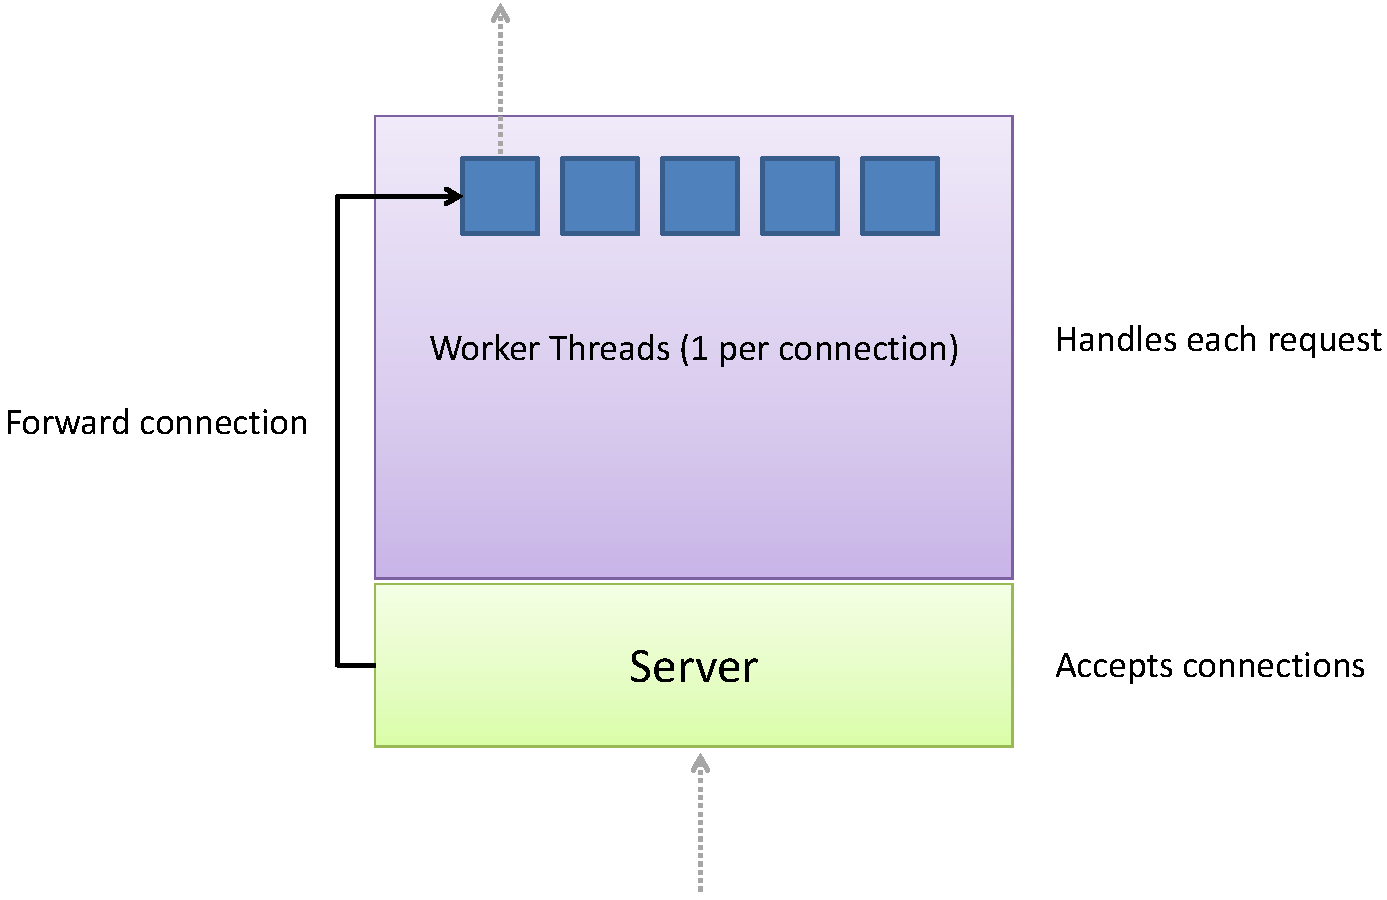
\includegraphics[width=0.75\textwidth]{webrick_architecture}
  \caption{WEBrick's request handling process}
  \label{fig:webrick_architecture}
\end{figure}
Due to its poor performance, users normally used alternate, less conventional setups which were also known for their lacking stability~\cite{ruby_webservers}.


\subsection{Mongrel}
Mongrel was released by Zed A. Shaw in 2006 and soon became the most popular web server in Rails production environments. It offered a much better performance when compared to WEBrick and it was reasonably suited for production environments. This was mainly due to its improved implementation of the HTTP parser, which was rewritten in C~\cite{mongrel_server_production}.

Similarly to WEBrick, Mongrel uses a single process. It has an acceptor thread which handles every incoming connections, launching new threads for each one of them. In production environments, Mongrel is commonly found in clustered configurations where several processes are launched and their usage is dictated by a proxy server~\cite{mongrel_faq}. Mongrel's request handling is demonstrated on figure~\ref{fig:mongrel_architecture}.
\begin{figure}[h]
  \centering
    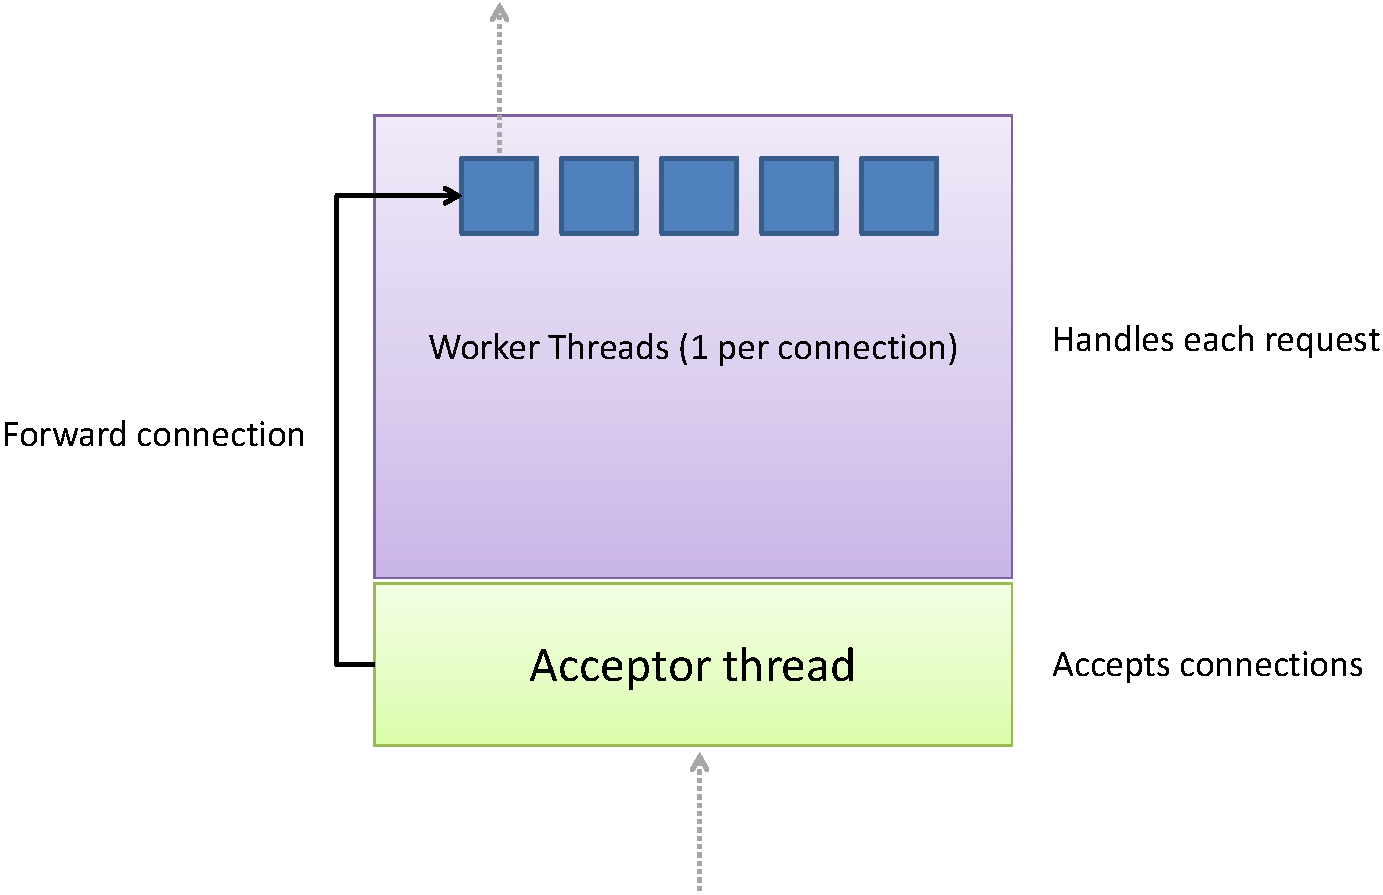
\includegraphics[width=0.75\textwidth]{mongrel_architecture}
  \caption{Mongrel's request handling process}
  \label{fig:mongrel_architecture}
\end{figure}
Mongrel also optimized the TCP stack by changing Ruby's default socket listening queue from 5 to 1024, besides using optimization flags on socket connections to improve bandwidth usage~\cite{mongrel_faq}.


\subsection{Thin}
Thin was released in 2008 and was the first Ruby web server which did not follow the \textit{one thread per request} convention. It uses Mongrel's HTTP parser and \textit{EventMachine} as its I/O back-end, allowing it to use a fast asynchronous event loop in a single thread for all incoming requests~\cite{thin}. Thin recently became able to combine threading with its philosophy, by allowing the creation of a background pool of 20 threads~\cite{ruby_webservers}. Thin is written in C, C++ and Ruby and is optimized for small requests and fast clients. Its request handling is demonstrated on figure~\ref{fig:thin_architecture}.
\begin{figure}[h]
  \centering
    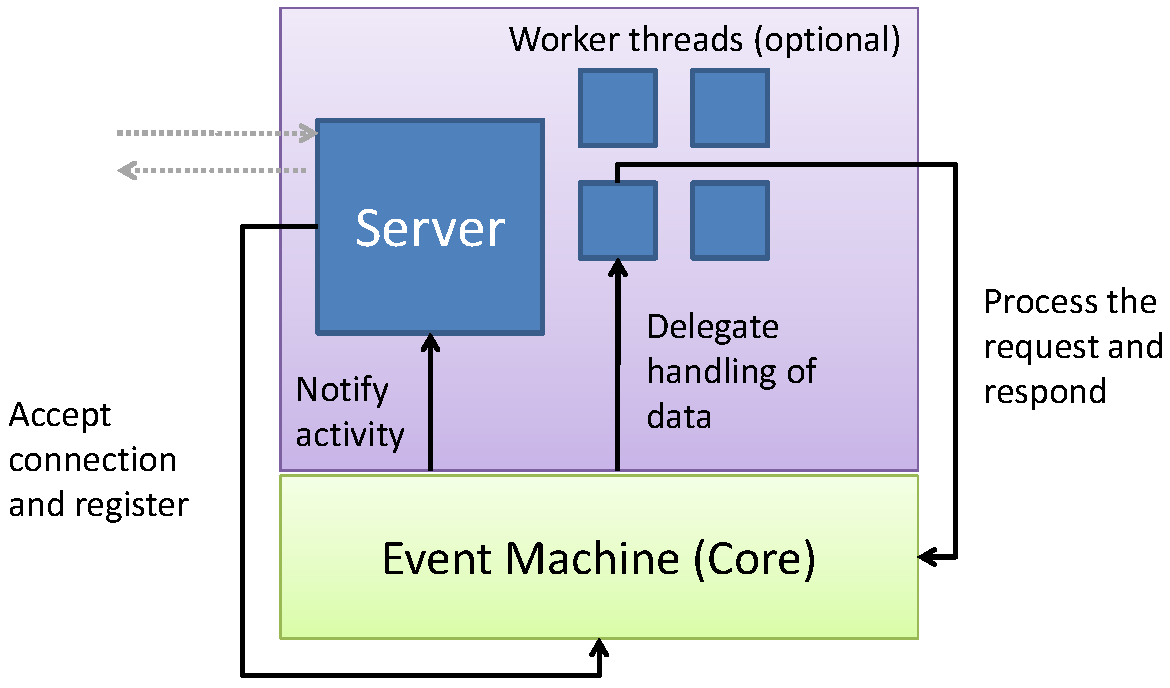
\includegraphics[width=0.75\textwidth]{thin_architecture}
  \caption{Thin's request handling process}
  \label{fig:thin_architecture}
\end{figure}
This setup yields better performance and scalability than Mongrel, especially when serving small requests like, for example, API calls. This is mainly related to the fact that this web server does not launch a new thread for each request, requiring less memory and no context switches~\cite{ruby_webservers}.
 
\subsection{Unicorn}
Unicorn's first stable version was released in 2009. It is a self-contained web server designed to take advantage of Unix-based kernels and is optimized for fast clients with low latency~\cite{unicorn}. It delegates every task that is better supported by the operating system, \textit{Nginx} or \textit{Rack} to themselves, respectively. It uses one master process that spawns and reaps a user-defined number of worker processes, without any thread usage. One of its main features is that load balancing is done by the OS kernel, avoiding that requests pile up behind a busy worker. Unicorn is written in Ruby, except for its HTML parser which is based on Mongrel's and, consequently, is written in C. When used in a production environment it should be deployed in conjunction with a reverse proxy capable of fully buffering both the requests and responses between itself and a slow client.
Unicorn's request handling is demonstrated on figure~\ref{fig:unicorn_architecture}.
\begin{figure}[h]
  \centering
    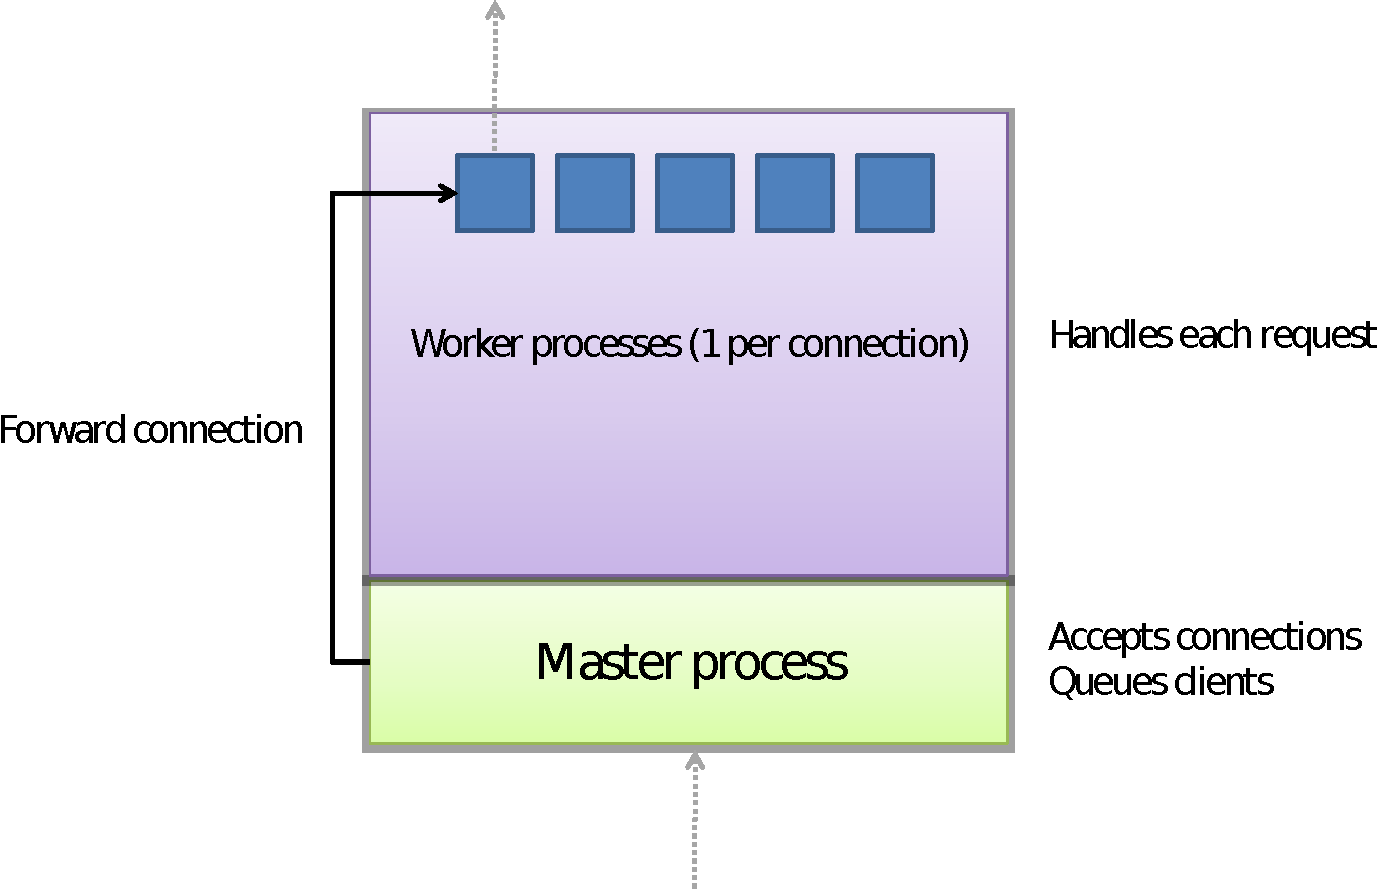
\includegraphics[width=0.75\textwidth]{unicorn_architecture}
  \caption{Unicorn's request handling process}
  \label{fig:unicorn_architecture}
\end{figure}


\subsection{Passenger}
Passenger was also released in 2008 but it had a big difference from the other options---it was not a self-contained web server. Passenger makes use of established web servers like Apache or Nginx by using their reliable web stack. It is mostly written in C++ and used as a module or extension to these generic web servers, adding the needed functionality to support Ruby and handling certain types of requests~\cite{passenger_whatis}.

When the web server starts, having Passenger loaded as a module, it launches a Ruby process that will be responsible for all the other processes handling the Ruby application, called the \textit{worker processes}. Each request is delivered to the firstly created Ruby processes---the master process---which forwards it to one of its workers. These worker processes are single threaded and handle one request at a time~\cite{ruby_webservers}. Passenger's request handling is demonstrated on figure~\ref{fig:passenger_architecture}.
\begin{figure}[h]
  \centering
    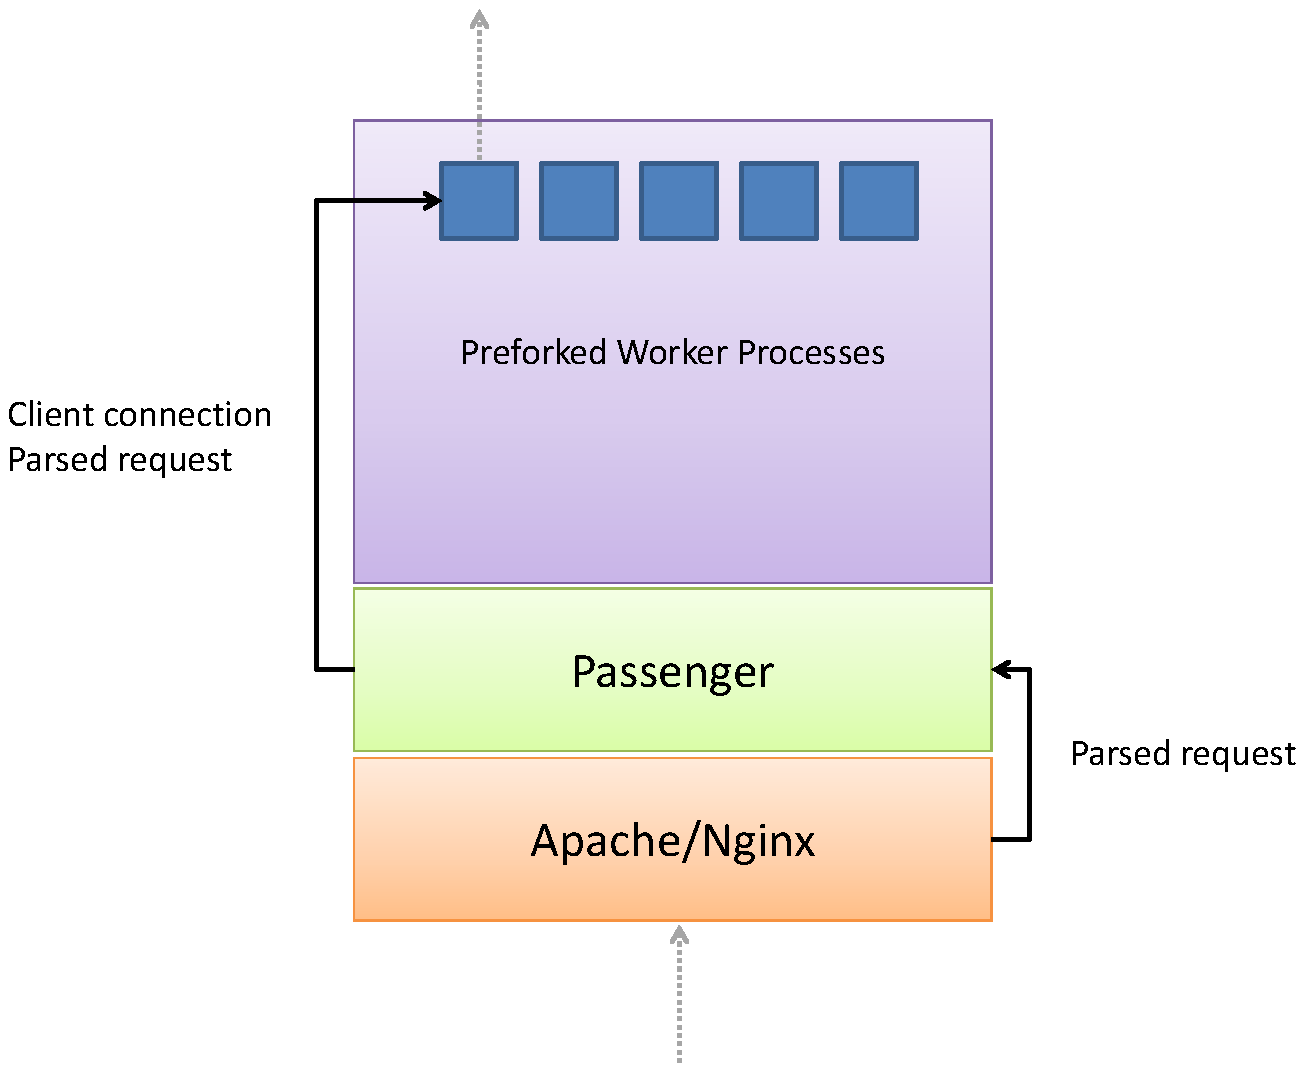
\includegraphics[width=0.75\textwidth]{passenger_architecture}
  \caption{Passenger's request handling process}
  \label{fig:passenger_architecture}
\end{figure}
It is the first real multi-process server for Ruby, although setups with multiple Mongrel or Thin servers were already being used~\cite{passenger_whatis}. Passenger is a free, open-source product but Phusion also provides commercial support.


\subsubsection{Apache}
The Apache HTTP Server is a full-featured and open source web server created by the Apache Software Foundation. It consists on a general purpose web server and provides many useful features such as HTTPS, IPV6 and authentication. Apache natively handles many languages such as PHP and Perl~\cite{apache_features}. It can be extended with modules and this is where Passenger comes in---it will act as \textit{mod\_rails} and extend Apache's functionality to be able to handle Ruby on Rails' applications~\cite{passenger_whatis}.


\subsubsection{Nginx}
Nginx is a general purpose lightweight open source web server with a strong focus on performance~\cite{nginx_features}. It was created by Igor Sysoevy and Passenger can extend its functionality by being installed as a module, similarly to the Apache's procedure~\cite{passenger_whatis}.

\section{Databases} % (fold)
\label{tech:sec:databases}
A database is a digitally organized collection of data. It can either be a schema-based or a schema-less database.

\subsection{MySQL}
MySQL is the most popular open source database in the world, having consistently fast performance, high reliability and ease of use~\cite{why_mysql}. It was first released in 1995 and it is the most commonly found database on a Ruby on Rails project. This is the database of choice for all \textit{37signals}'s applications~\cite{interview_dhh}.  It is a relational schema-based database that offers useful features like various storage engines, transactions, indexes, load balancing and many others.

MySQL's architecture consists in three main layers. The top one is related with the services that are not unique to MySQL, like connection handling, authentication and security. The middle layer refers to crucial MySQL features like query parsing, analysis, optimization, caching and all the built-in functions.  This layer also holds all functionality across storage engines and stored procedures. Finally, the bottom layer consists in the storage engines themselves, responsible for the storage and retrieval of all stored data~\cite{high_performance_mysql}. MySQL has four main storage engines---MyISAM, Heap, BDB and InnoDB---with distinct advantages and disadvantages. However, InnoDB is the only storage engine supported in Rails applications. MyISAM and Heap lack transaction support and BDB does not ensure referential integrity, features used by the Ruby on Rails framework. Nevertheless, InnoDB is the default storage engine on MySQL installations.

Ruby has an official library for this database, called \textit{mysql}. There are, however, a few alternatives worth mentioning, namely \textit{mysql2} and \textit{mysqlplus}. These two have some similar and a few other distinct goals:
\begin{description}
  \item[\textit{mysql2}] aims at performing the necessary type conversions between MySQL and Ruby types in C and allows asynchronous queries.
  \item[\textit{mysqlplus}] aims at supporting asynchronous queries and enabling threaded database access.
\end{description}

The installation of \textit{mysql2} automatically patches ActiveRecord, allowing a smooth transition from the default library. The other mentioned alternative, \textit{mysqlplus}, also replaces the default driver and does not need patching to natively interact with ActiveRecord.


\subsection{PostgreSQL}
PostgreSQL is the most advanced open source database server. It was started by Michael Stonebraker at the University of California in Berkeley and had its first release in 1989. It is a DBMS that contains all features found on other open source or commercial databases and a few more~\cite{beginning_postgresql}.

PostgreSQL has some prominent users, like \textit{MySpace}, who strengthen its credibility as a full-featured scalable highly-reliable relational database~\cite{petabyte_warehouses}. Rails' ActiveRecord natively supports this type of database, using Ruby's official library---\textit{ruby-pg}.


\subsection{MongoDB}
MongoDB is a scalable, highly performant, open source, schema-free, document-oriented database written in C++ whose first release was in early 2009. It is a combination of key-value stores, fast, highly scalable and traditional RDBMS systems which provide structured schemas and powerful queries.

This database is document-oriented, providing the simplicity and power of JSON-like data schemas. It supports dynamic queries and indexes. It also provides complex features like replication, auto-sharding and MapRedux~\cite{mongodb}

This database has been gaining popularity within the Rails community for its simplicity of use, high performance and many features that fit well within the Ruby development philosophy~\cite{mongodb_rails}. Mongo is very performance-oriented and some of its features that provide outstanding performance are~\cite{mongodb_couchdb}:
\begin{itemize}
  \item Client driver per language: native socket protocol for client/server interface;
  \item Use of memory mapped files for data storage;
  \item Collection-oriented storage (objects from the same collection are stored contiguously);
  \item Update-in-place;
  \item Written in C++.
\end{itemize}
Rails does not natively support MongoDB. For its usage in Rails the developer must replace its default ORM, \textit{ActiveRecord}, with \textit{MongoMapper}. This library provides access to Mongo database operations and natively supports Ruby objects without conversions~\cite{mongomapper}.



\section{Ruby on Rails} % (fold)
\label{tech:sec:ruby_on_rails}
David Hansson began working on a web-based project management tool oriented towards small teams in 2003. At \textit{37signals} he initially started by using PHP but soon became frustrated by many of the language's shortcomings. He gave up on this language and started implementing what today is known as \textit{Basecamp} in pure Ruby. While developing the application, he noticed that a lot of its code could be extracted into a framework for future use with other applications. Hansson decided to release his framework to the public in July 2004 and Ruby on Rails was born~\cite{railssolutions}.

Rails started to become more mature over time and applications like Twitter, YellowPages, Hulu, Scribd and GitHub were built using this framework. Its popularity has grown significantly since the beginning and its adoption by popular platforms helped establishing Rails as a solid framework.

Ruby on Rails has three main principles which motivated its creation~\cite{agile_webdevelopment_with_rails, ruby_on_rails_principles}:
\begin{description}
\item[Convention over configuration.] In Rails, everything has a default configuration. The only exception is the database connection data. This way, developers only need to specify when they want to use unconventional configurations. This way, Rails offers simplicity while retaining significant flexibility.
\item[Don't Repeat Yourself.] Also known as DRY, this practice implies that the similar code snippets do not exist in separate locations. Every piece of knowledge is unique, definite and has a relevant representation. This simplifies modifications by the avoidance of having to change the same logic in different parts of the project, allowing the applications to keep a high consistency degree.
\item[Model-View-Controller.] Rails follows the MVC architecture pattern, keeping the source code well organized by clearly separating the code according to its purpose. The \textit{Model} is responsible for maintain the state of the application, specifying the constraints its related data has to obey to. The \textit{Controller} receives the users' input, interacts with the model and finally renders a view page as the result. The \textit{View} can have multiple formats, from JSON to XML, and is essentially what is displayed to the users. This principle's schema is presented in figure~\ref{fig:mvc}.
\begin{figure}[h]
  \centering
    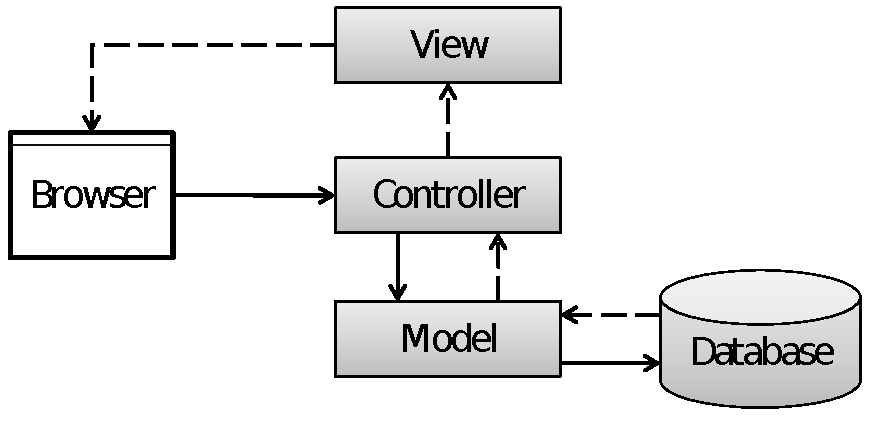
\includegraphics[width=0.75\textwidth]{mvc}
  \caption{Model-View-Controller architectural pattern}
  \label{fig:mvc}
\end{figure}\\
\end{description}
Rails' functionality can be altered and extended with plugins. While being a full stack web framework, Rails does not aim to include every single feature. However, it has been built with a highly extensible infrastructure and it has a considerably large set of plugins nowadays~\cite{rails_magazine_1}.


\subsection{Rails 2}
\label{tech:sec:ruby_on_rails:rails2}
Rails 2 was first released in 2007 and is currently in version 2.3, released at the beginning of 2009. Throughout these 2 years the framework was improved by many contributors, aside from the core team~\cite{rails_core_team}. The framework is essentially divided in six essential modules~\cite{ruby_on_rails_principles, rails23_release_notes}:
\begin{description}
\item[ActionPack] splits the response in two:  a request for the controller to handle the login and a template rendering part for the view to handle.
\item[ActiveRecord] is responsible for object handling and their database representation. Objects are directly linked to the database, so modifying them will modify the table definition they are associated with.
\item[ActiveResource] corresponds to objects that represent the application's RESTful resources as manipulatable Ruby objects.
\item[ActiveSupport] is a collection of various utility classes and standard library extensions.
\item[ActionMailer] is a framework for designing email-service layers, allowing the application to send emails using a mailer model and views.
\end{description}
Rails has a lot of modules and classes but everything is structured using the aforementioned components.


\subsection{Rails 3}
\label{tech:sec:ruby_on_rails:rails3}
Rails 3 is currently in development and it is on its first release candidate, after four beta versions. Most of Rails' code has been refactored and this release's main goals were concerned with improved component decoupling and performance~\cite{rails3_great_decoupling}. 

As of component decoupling, a great deal of work has been done and impressive goals have been achieved~\cite{vaporware_to_awesome}. Most of Rails' components are agnostic now, having standard interfaces for communication with each other. The key concept is that a component is agnostic to whom it is interacting with. This allows component swapping, enabling the replacement of one or more of Rails' core components with a different, third-party one. In order to make this happen standard procedures have been developed, providing standard interfaces for each one of Rails' components.

The decoupling process also allowed for improved modularity, permitting Rails' component separation. ActionController, for instance, has been split into ActionDispatch, ActionController and AbstractController~\cite{vaporware_to_awesome}. There was a lot of work on explicitly handling each component's internal dependencies. This enables the developer to carefully select which modules he needs in his Rails application without caring about including the modules it depends on as well. In previous versions of Rails developers would import the top-level modules, since the alternative was to parse the source code of the framework to find its internal dependencies in order to import all necessary modules. Applications are now able to only load the modules they really need thus becoming faster and lighter.

This improved modularity also had its impact on performance. However, the team also made a specific effort into improving common Rails bottlenecks like partial and collection rendering~\cite{vaporware_to_awesome}, among some other optimized sections.


% chapter technologies (end)

  %% State Of The Art
  \chapter{State of the Art} % (fold)
\label{cha:state_of_the_art}
\headermark{State of the Art}

\section*{} % (fold)
Each component's state of the art will be presented in this chapter, providing an analysis of related work.
% section  (end)

\section{Operating Systems} % (fold)
\label{state:sec:operating_systems}

This research is focused on server environments since deployed Ruby on Rails applications are commonly found in these setups. When it comes to servers, thought, the emphasis on performance becomes much more critical since it is a very important requirement that applications demand from this kind of environment. Some facts suggest that the most commonly found performance bottlenecks in servers are related to the operating system. Operating systems performance bottlenecks usually reside in three key issues~\cite{os_performance_server}:
\begin{itemize}
\item Process management;
\item Virtual memory management;
\item High performance I/O.
\end{itemize}
Each operating system addresses bottlenecks differently and their decisions impact application specific and system-wide performance.

In this research's context, performance is addressed from a Ruby on Rails perspective. Windows' support for this framework and related components is poor and this environment makes the framework slower. Passenger, one of the major Rails web servers used in production, opted not to support the Windows platform. As Marcus Koze explains~\cite{marcus_koze_passenger}:
\begin{quote}
  ``We have no plans to port Passenger on Windows. Windows lacks the proper facilities to implement Passenger efficiently. Passenger on Windows will be very, very inefficient, which can give both Ruby on Rails as well as Passenger a bad name.''
\end{quote}
Many other web-oriented benchmarks show that Linux has better scalability and performance compared to Windows when it comes to this type of servers~\cite{apache_tomcat_performance_linux_windows, php_apache_linux_windows}. The difference is quite noticeable: Ruby on Rails is still more efficient in a Virtual Machine running Linux than in a normal installation of Windows~\cite{linux_virtualbox_windows_rails}.

Documentation on how to use and deploy Rails applications in the Windows platform is also scarce, often needing unconventional methods for being able to run it properly~\cite{rails_windows}.

Since Rails is built on top of the Ruby programming language, this framework's lack of performance in Windows is possibly related to the poor Ruby performance in this operating system. The Ruby 1.8 official interpreter is twice as fast in Linux than its Windows counterpart. As of YARV, the Ruby 1.9 official interpreter seems to be 70\% faster on Linux when compared to its Windows counterpart~\cite{ruby_faster_linux}. Windows-specific Ruby interpreters do not seem to have noticeable performance improvements~\cite{ruby.net} and lack the necessary stability and compliance with the Ruby specification. \textit{IronRuby}, for instance, is an interpreter developed by Microsoft~\cite{ror_ecosystem_whitepaper} that is faster than Windows' MRI but still slower than the YARV implementation for this operating system. It also presents stability issues, as timeouts are common in a considerable number of benchmarks~\cite{ironruby_performance}.

On a side note, MySQL's documentation states that there are a few unpleasent details when using this database under a Windows environment~\cite{mysql_windows_linux}. First of all, it is only conceded 4000 ports which after being used need two to four minutes before becoming available again. It also has a limited allowed opened files number---2048---restraining its concurrent capabilities. Finally, MySQL uses a blocking read for each connection and Windows' connection error handling is quite poor when compared to Linux's counterpart. As the aforementioned documentation states, all these differences limit the number of acceptable concurrent requests handled and difficult high-load handling. They can lead to performance issues and limit the system's scalability.

To date, there are no specific tests analyzing Ruby on Rails' performance on BSD when compared to other operating systems. However, many web discussions suggest that it is quite similar to the one achieved on Linux which is understandable since they are both \textit{UNIX} derivates.

\section{Ruby} % (fold)
\label{state:sec:ruby}
The Ruby on Rails framework, as its name implies, is built on top of the Ruby programming language. Rails' performance is highly affected by Ruby and the interpreter choice can lead to great impact on the framework's scalability.

Ruby has many interpreters according to its version. Ruby 1.8 has MRI as its default interpreter and Ruby 1.9 has YARV. There are, however, a few other implementations that start to deserve some attention. These present different philosophies and implementation details that provide them with a few advantages and other shortcomings. The most popular Ruby interpreters for Ruby 1.8 are as follows:
\begin{description}
\item[MRI,] the standard Ruby 1.8 interpreter.
\item[Ruby Enterprise Edition,] based on the MRI's code but modified for better performance in Rails environments.
\item[JRuby,] a Ruby interpreter built on top of JVM.
\item[Rubinius,] a promising Ruby interpreter built by Rails' creators --- \textit{EngineYard}.
\end{description}
Version 1.9 came out recently so alternative interpreters do not fully support it just yet. YARV, the standard Ruby 1.9 interpreter, is the only one to support the specification.

The default implementation for Ruby 1.8, MRI, is generally known by its poor performance~\cite{6tips_for_mri}. This motivated the development of efficient interpreters for the language. Ruby Enterprise Edition has better scaling abilities than MRI, generally performs better and uses less memory~\cite{ree_benchmarks}. JRuby outperforms MRI by a considerable margin~\cite{ruby19_performance}. Rubinius, on the other hand, also effortlessly outperforms MRI. It also performs better than JRuby in most cases but by a much smaller margin~\cite{rvm_rubinius_benchmarks}.

Some people found significant performance improvements in MRI by applying a series of patches and configurations to its garbage collector. Twitter benefited from this patches, roughly improving its overall performance by 30\%~\cite{ruby_gc_tuning}.

Ruby 1.9 has only one compliant interpreter as aforementioned. However, as reference benchmarking, its performance is better than JRuby's~\cite{ruby19_performance}  and is paired with Rubinius'. It performs slightly better in some benchmarks but also performs faintly worse on others~\cite{rvm_rubinius_benchmarks,ruby_interpreter_benchmarks}. Some people even got as far as saying it was more efficient than Python's counterpart~\cite{ruby19_python}.


\section{Rails Web Servers} % (fold)
\label{state:sec:rails_web_servers}
The first Rails web server was WEBrick, publicly released in 2000. Mongrel came in 2006 and soon after Thin and Passenger followed.

Using the aforementioned web servers, Muhammed Ali did an extensive overview of some characteristics that heavily contribute to web server performance~\cite{ruby_webservers}. Muhammed's analysis is exposed in the following sections, along with a brief overview of how each web server handles them.

\subsection{Data Copying}
When a server fetches a file from the disk or a back end server it usually copies it to kernel space in order to send it to the client. There are ways of sending the data directly without copying it, called \textit{zero-copy} techniques~\cite{ zero-copy_data_transfer}.

WEBrick, Mongrel and Thin neglect this issue. Passenger neglects it as well but, on the other hand, it passes file descriptors to worker processes which avoids sending the data to the clients through the parent web server.

\subsection{Context Switching}
This issue is related with context switching between kernel and user space and all the overhead involved in this procedure. System calls and thread exchange are some of the activities that cause context switches.

WEBrick and Mongrel highly rely on threads, which implies many context switches. In Passenger's case, context switches are related to process context switching, since it uses processes instead of threads. Thin efficiently handles context switches---it does not use threads nor processes, reducing the impact of this issue.

\subsection{Lock Contention} 
Multiple threads or processes with shared data imply data locking from time to time. If the data is locked it will put the remaining threads or processes trying to use it on hold.

WEBrick's and Mongrel's threads share almost no data, avoiding noticeable issues related to lock contention. Neither Thin nor Passenger share data inter processes or threads, completely avoiding lock contention.

\subsection{Memory Management}
Web servers allocate and free memory frequently and Ruby's garbage collector is not very efficient for such application behavior. Web servers might counter this issue by allocating little objects and/or reusing them as much as possible.

WEBrick does not conserve memory neither reuses objects. In Mongrel, though, parser objects are reusable and string usage is kept to a minimum, being replaced by constants. Thin also avoids using strings in detriment of constants but buffers data twice in memory before retrieving it from \textit{Rack}. Passenger does an excellent job in memory management by using the fork friendly Ruby implementation, allowing it to recycle worker processes.

\subsection{Blocking Operations}
I/O operations, as mentioned before, block the server until the operation finishes.

WEBrick solely relies on non-blocking I/O. Contrary, Mongrel performs all I/O in a blocking manner because of its usage of threads. Thin, on the other hand, does most of its I/O operations in a non-blocking manner and Passenger is not affected by this issue since it uses single threaded processes.

\subsection{HTTP Parsing}
The implementation of the HTTP parser greatly affects the web server performance since it is a heavy procedure.

WEBrick's HTTP parser is written in pure Ruby, having poor performance. Mongrel, in contrast, uses a fast and secure implementation written in C. While Thin uses a similar parser to Mongrel's one, Passenger does not do HTTP parsing and handles that responsibility to its underlying web server.

\subsection{TCP Stack}
Web servers can tune TCP operations by specifying a set of options allowed by the TCP protocol implementation.

WEBrick and Thin do not try to optimize the TCP stack while Mongrel uses two configuration options that increase the number of allowed waiting connections and \textit{TCP\_CORK} to optimize bandwith usage. Finally, these kinds of optimizations on Passenger depend on whether its underlying web server is using TCP stack optimization configurations.\\\\% FIXME: hack :|
From all the exposed Rails web servers, Passenger presents itself as the easiest to setup in a server environment~\cite{ruby_webservers} since it can be installed as a module for other easily installable web servers like Apache or Nginx.

\subsection{Benchmarks}
Some benchmarks were endured by Muhammed Ali~\cite{ruby_webservers}, whose results are showed on table~\ref{tab:webserver_benchmarks}.
\begin{table}[h!t]
  \centering
  
  \begin{tabular}{p{1.3cm}|p{1.8cm}|p{2cm}|p{2cm}|p{2cm}|p{1.3cm}|p{2cm}}
    \textsc{Test}
  & \textsc{Users}
  & \textsc{Requests}
  & \textsc{WEBrick}
  & \textsc{Mongrel}
  & \textsc{Thin}
  & \textsc{Passenger} \\
  \hline

  \multirow{3}{*}{1}
  & 10 & 1000 & 169 & 438 & 650 & 497\\
  & 100 & 1000 & 209 & 451 & 613 & 509\\
  & 1000 & 1000 & 250 & 446 & 615 & 324\\
  \hline
    
  \multirow{3}{*}{2}
  & 10 & 1000 & 115 & 309 & 365 & 305\\
  & 100 & 1000 & 165 & 299 & 350 & 316\\
  & 1000 & 1000 & 194 & 284 & 346 & 307\\
  \hline
  
  \multirow{2}{*}{3}
  & 10 & 1000 & 41 & 44 & 43 & 45\\
  & 100 & 1000 & 41 & 42 & 45 & 44\\
  \hline

  \multirow{2}{*}{4}
  & 10 & 1000 & 41 & 37 & 55 & 79\\
  & 100 & 1000 & 41 & 37 & 54 & 79\\
  \hline
  
  \multirow{2}{*}{5}
  & 10 & 1000 & 6 & 5 & 7 & 10\\
  & 100 & 1000 & 6 & 5 & 2 & 10\\
  
  \end{tabular}
  \caption{Web server benchmark results}
  \label{tab:webserver_benchmarks}
\end{table}
All tests consist in serving dynamic requests from a single Rails process. All requests are made concurrently and each web server's results are in number of requests handled per second. Test 1 is a sample ``Hello World!'' page. Test 2 fetches a database record and renders it as an ERB template. Test 3 marshals 500 complex objects. Test 4 sends a large 1MB response. Finally, test 5 sends a very large 10MB response.

According to Muhammed's analysis, WEBrick is evidently slow when compared to its counterparts. Mongrel performs much better that its ancestor and both Thin and Passenger improve over it. Thin is clearly the best web server for serving small requests. Passenger, though, is the one to scale better since it performs similarly with 10 or 1000 concurrent users. It also shows better performance when handling large responses. Its performance could be different if it was using Nginx as its back-end instead of Apache.

Unicorn was not contemplated on the previously shown tests but it has been gaining reputation and its adoption is increasing. \textit{Twitter}, the problematic platform mentioned before, recently switched over to Unicorn as its web server, publicly praising some of its features. Among them are its request queue handling, master/slaves architecture, error encapsulation and recovery, CPU usage and a feature called \textit{zero-downtime deployment} that ``works beautifully''~\cite{twitter_unicorn}.


\section{Databases} % (fold)
\label{tech:sec:databases}
A database collects data, either records or files. From the Rails perspective, this can either be a schema-based or a schema-less database.


\subsection{MySQL}
MySQL is the most popular open source database in the world, having consistently fast performance, high reliability and ease of use~\cite{why_mysql}. It was first released in 1995 and it is the default database on a Ruby on Rails project. This is the database of choice for all \textit{37signals}'s applications~\cite{interview_dhh}.  It is a relational schema-based database that offers useful features like various storage engines, transactions, indexes, load balancing and so on.

Figure~\ref{fig:mysql_architecture} presents a simple overview over MySQL's architecture.
\begin{figure}[h]
  \centering
    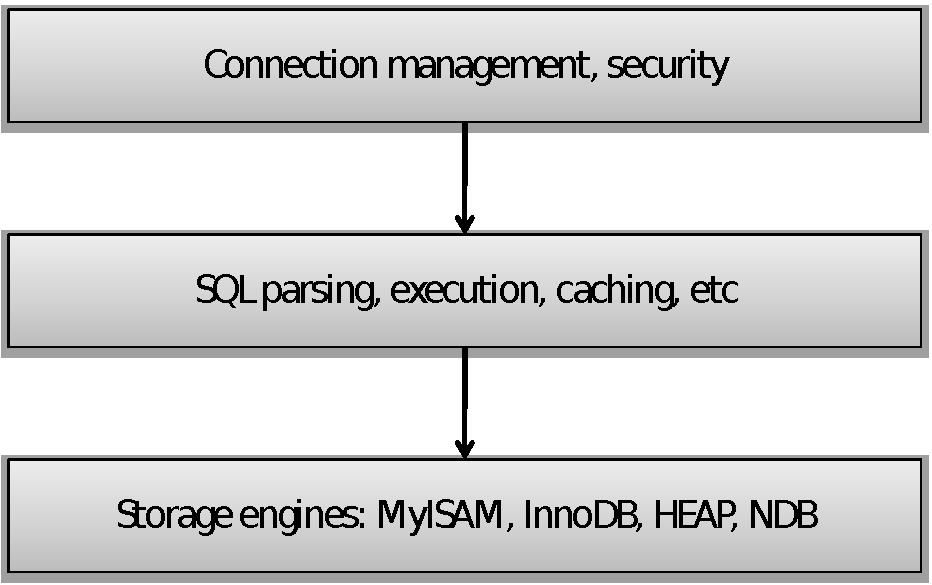
\includegraphics[width=0.75\textwidth]{mysql_architecture}
  \caption{Logical view of MySQL's architecture}
  \label{fig:mysql_architecture}
\end{figure}
The top layer is related with the services that are not unique to MySQL, like connection handling, authentication and security. The middle layer refers to crucial MySQL features like query parsing, analysis, optimization, caching and all the built-in functions.  This layer also holds all functionality across storage engines and stored procedures. Finally, the bottom layer consists in the storage engines themselves, responsible for the storage and retrieval of all stored data~\cite{high_performance_mysql}. MySQL has four main storage engines, all with advantages and disadvantages, the default one being InnoDB.

A high-level summary of the characteristics of all four storage engines can be found on table~\ref{tab:storage_engines_mysql}.
\begin{table}[ht]
  \centering
  
  \begin{tabular}{p{4cm}|p{2cm}|p{2cm}|p{3cm}|p{2cm}}
    \textsc{Attribute}
  & \textsc{MyISAM}
  & \textsc{Heap}
  & \textsc{BDB}
  & \textsc{InnoDB} \\
  \hline

    \textbf{Transactions}
  & No
  & No
  & Yes
  & Yes \\

  \hline
    \textbf{Lock granularity}
  & Table
  & Table
  & Page
  & Row \\

  \hline
    \textbf{Storage}
  & Split files
  & In-memory
  & Single file per table
  & Tablespace \\

  \hline
    \textbf{Isolation levels}
  & None
  & None
  & Read committed
  & All \\

  \hline
    \textbf{Portable format}
  & Yes
  & No
  & No
  & Yes \\

  \hline
    \textbf{Referential integrity}
  & No
  & No
  & No
  & Yes \\

  \hline
    \textbf{Primary key with data}
  & No
  & No
  & Yes
  & Yes \\
    
  \hline
    \textbf{MySQL caching}
  & No
  & Yes
  & Yes
  & Yes \\

  \hline
    \textbf{Available versions}
  & All versions
  & All versions
  & MySQL-Max
  & All versions \\
  \end{tabular}
  \caption{Storage engine characteristics in MySQL}
  \label{tab:storage_engines_mysql}
\end{table}
Rails' ActiveRecord natively supports this type of database.


\subsection{PostgreSQL}
PostgreSQL is the most advanced open source database server. It was started by Michael Stonebraker at the University of California in Berkeley and had its first release in 1989. It is a DBMS that contains all the features found on other open source or commercial databases and a few more. Some of these features include~\cite{beginning_postgresql}:
\begin{itemize}
  \item Transactions;
  \item Subselects;
  \item Views;
  \item Foreign key referential integrity;
  \item Sophisticated locking;
  \item User-defined types;
  \item Inheritance;
  \item Rules;
  \item Multiple-version concurrency control;
  \item Native Microsoft Windows version;
  \item Table spaces;
  \item Ability to alter column types;
  \item  Point-in-time recovery.
\end{itemize}
PostgreSQL has some prominent users, like MySpace, who strengthen its credibility as a full-featured scalable highly-reliable relational database~\cite{petabyte_warehouses}. Rails' ActiveRecord natively supports this type of database.


\subsection{MongoDB}
MongoDB is a scalable, high performance, open source, schema-free, document-oriented database written in C++ whose first release was in early 2009. It is a combination of key-value stores, fast and highly scalable, and traditional RDBMS systems which provide structured schemas and powerful queries. Among other features, MongoDB provides~\cite{mongodb}:
\begin{itemize}
  \item Document-oriented storage (the simplicity and power of JSON-like data schemas);
  \item Dynamic queries;
  \item Full index support, extending to inner-objects and embedded arrays;
  \item Query profiling;
  \item Fast, in-place updates;
  \item Efficient storage of binary data large objects (e.g. photos and videos);
  \item Replication and fail-over support;
  \item Auto-sharding for cloud-level scalability;
  \item MapReduce for complex aggregation.
\end{itemize}
This database has been gaining popularity within the Rails community for its simplicity of use, high performance and many features that fit well within the Ruby development  philosophy~\cite{mongodb_rails}. Mongo is very performance oriented and some of its features that provide outstanding performance are~\cite{mongodb_couchdb}:
\begin{itemize}
  \item Client driver per language: native socket protocol for client/server interface (not REST);
  \item Use of memory mapped files for data storage;
  \item Collection-oriented storage (objects from the same collection are stored contiguously);
  \item Update-in-place (not MVCC);
  \item Written in C++.
\end{itemize}
Rails' ActiveRecord does not natively support MongoDB. For its usage in Rails the developer must use \textit{MongoMapper}, which provides access to Mongo database operations and natively supports Ruby objects without conversions~\cite{mongomapper}.


\section{Ruby on Rails} % (fold)
\label{state:sec:ruby_on_rails}
Rails' development is mainly done by its creators --- \textit{37signals} --- and so are its performance optimizations. However, many companies like Twitter had the need to squeeze this frameworks scalability and focused on some identified critical bottlenecks like Ruby's garbage collector mentioned in section~\ref{state:sec:ruby}.

There have been some outside performance improvements over Rails 2.3 code, though. From simple Rails' source minor patching~\cite{accunote_rails} to complete architecture makeovers ~\cite{distributed_rails}, Ruby on Rails' improvement attempts were widely made.

However, the main performance improvements over Rails 2.3 can be found in Rails 3. The decoupling mentioned in section~\ref{tech:sec:ruby_on_rails:rails3} improved Rails performance and scalability, allowing faster execution times and lighter memory usage.

There were also specific performance optimizations, namely on \textit{partial} and \textit{collection} handling. Controller code was also refactored to become lighter. Initial performance benchmarks show that partial and collection rendering and overall performance is more than two times faster~\cite{rails_merb_merge_performance, vaporware_to_awesome}.


% chapter state_of_the_art (end)

  %% State Of The Art
  \chapter{Problem Statement} % (fold)
\label{cha:problem_statement}
\headermark{Problem Statement}

\section*{} % (fold)
Ruby on Rails applications generally have scalability issues. A significant amount of applications developed using this framework exhibit this issue by publicly starting to suffer from performance and scalability issues as their popularity increases. The Ruby on Rails community is not generally focused in building highly performant systems. The lack of generic centralized information, functional and intuitive profiling tools and global awareness of this subjects's importance all contribute to this problem.

As observable on chapter~\ref{cha:state_of_the_art}, some information regarding benchmarks and configurations of the various components involved in a Rails application exists but it is, however, very scattered. Most tests and configuration evaluations are not generic, focusing on specific components, setups or purposes. It is crucial to create a solid set of conventions and guidelines that are generic and cover all components, approaching benchmarking and tweaking from a unified perspective---optimizing a Ruby on Rails application.

On a related matter, the native profiling tools in Ruby on Rails have never functioned properly when used with Ruby 1.9. While complicating the act of profiling an application, this also prevents some users from switching to this version and leveraging from its increased performance. At the same time, the profiling output formats supported are all text based. Profiling is an essential aspect of increasing an application's performance, so it is very important to fix Ruby and Rails' profiling tools, provide a seamless integration between them and the most recent versions of Ruby and add support for alternate, more intuitive profiling output formats.

As mentioned in chapter~\ref{cha:introduction}, Twitter---and a few other renowned platforms---had many scalability issues which were not discrete, some becoming quite famous. However, the global awareness of the Ruby on Rails community regarding the importance of scalability is still remarkably low. Despite having the Rails 3 API available shortly after its development began back in early 2009 and Ruby 1.9 available since 2008, most plugin developers have not added support for these versions to their plugins. Famous Rails applications, like Redmine, also lack support for Ruby 1.9 and have not started upgrading to Rails 3. Knowing the performance benefits of using the latest versions of both components, it is important to increase the community's \textit{momentum} by updating famous plugins and applications, possibly igniting an update-focused philosophy.

To create a generic guideline with centralized information, improve the current profiling tools and increase the community's sensibility on this subject it is crucial to address specific characteristics, configurations and issues of all components involved with the aforementioned perspective. 

The following sections state and justify the problems addressed in each component.

\section{Operating Systems}
Focusing on finding specific Operating System bottlenecks and solving or improving them is beyond the scope of this project. It is also unlikely to be worthwhile given the time span of the project and its wide area coverage. Furthermore, most operating systems have significant communities discussing, implementing and improving solutions to given bottlenecks.

However, there is need to determine which OS is best suited for Rails applications. The lack of generic benchmarking tools limits one's ability to fairly compare the performance of operating systems. These should be created, taking into account common tasks performed by them. 

Ascertaining which OS best handles web server load with the default configurations is also important to build a starting point for deploying and optimizing Rails applications. 

Finally, as mentioned in section~\ref{tech:sec:ruby}, Ruby is mainly developed in Linux but should easily run on many other operating systems. However, as seen on section~\ref{state:sec:operating_systems}, its performance can greatly differ depending on what OS is running it. The analysis on the performance differences of the Ruby interpreters across operating systems should continue, aside from those already determined.

\section{Ruby}
Ruby 1.9 is supposed to have a noticeably better performance than its ancestor. Most Rails applications were developed with version 1.8 and would highly benefit from the new version's improvements if they were upgraded. It is crucial to determine the benefits of this upgrade to justify the effort needed to accomplish it. 

As explained in section~\ref{state:sec:ruby}, most of the Ruby-related performance bottlenecks found in Rails applications are related to its garbage collector. Despite using a not very optimized garbage collection algorithm---\textit{mark-and-sweep}---it is not configurable, lacking the ability to adapt itself to the application it is running. As seen on section~\ref{tech:sec:ruby}, there are many benefits in having a configurable GC, so it becomes important to give YARV this flexibility. 

Finally, the integration between Rails' profiling and benchmarking tools and Ruby is outdated or, in some cases, nonexistent. It is important to update the existing tools and add support for new information and output formats, therefore improving YARV's data retrieval abilities and its integration with Rails' profiling and benchmarking facilities.

\section{Rails Web Servers}
There are many analysis concerning web server performance but unfortunately most of them are either outdated, not applicable nowadays' setups, not covering a wide range of web servers or lacking relevant data. For instance, the high quality analysis mentioned in~\ref{state:sec:rails_web_servers} does not include Unicorn, nor does it test Mongrel, Passenger and Thin behind other web servers. Furthermore, one of the critically significant but frequently missing aspect in benchmarks is memory usage.

It is also important to analyze the high-load response of each web server by stressing it to its limits and evaluating its behavior from a stability perspective. 

An up-to-date analysis covering raw performance, high-load stability and memory usage is crucial for increasing developers' awareness of the benefits and shortcomings of each web server setup. Since most web servers are natively flexible and configurable, its essential to explore and analyze their configuration options as well.

\section{Databases}
Similarly to the OS component, focusing on finding specific Database bottlenecks and solving or improving them is beyond the scope of this project. It is also unlikely to be worthwhile given the previously stated reasons.

However, Ruby plays an important role concerning databases. The current implementation of the \textit{mysql2} library converts the data between MySQL types and Ruby objects immediately after fetching each row from the database. This behavior is not optimal for situations where there are more fields being fetched than those being used. Changing the program's flow in order to trigger type casting only when the variable is actually accessed---lazy type casting---can have a significant impact on the aforementioned conditions, becoming an important issue to address.

This library is likely to replace Ruby's default in the future. It is being actively developed and provides significant ameliorations from the current library, \textit{mysql}. It is starting to gain a solid reputation within the Ruby community, posing as an excellent target for improvements concerning this component.

\section{Ruby on Rails}
The current native profiling tools for Ruby on Rails are deprecated. They do not function properly on up-to-date environments and they highly depend on Ruby's profiling abilities which are very limited. Improving Ruby's profiling tools is not enough as they need to seamlessly integrate with Rails'. For this to happen, Rails must also targeted for improvements by refactoring and improving the existent non-functional profiling tools.

Rails 3's performance is significantly better when comparing to its predecessor, as mentioned in section~\ref{state:sec:ruby_on_rails}. However, the adoption of Rails 3 will probably be difficult and lengthy since applications need to be refactored and most plugins---one of the main advantages of this framework as explained in section~\ref{tech:sec:ruby_on_rails}---need to be rewritten. To motivate its early adoption and increase this version's \textit{momentum}, some of the most famous plugins need to be ported to the new version. Getting one of the most famous applications---Redmine---to work properly on Rails 3 would also increase the awareness of the new versions' benefits. Finally, some performance bottlenecks commonly found in Rails applications for whose simple solutions exist should also addressed.

\begin{comment}
Rails scalability should be easily accessible to everyone

Improve existing tools, create/improve measurement tools

Missing performance-oriented guidelines and conventions

Missing and out-dated tools to profile Rails applications

Optimal configurations and setups
\end{comment}

  %% Problem Approach and Results
  \chapter{Problem Approach and Results} % (fold)
\label{cha:problem_approach_and_results}
\headermark{Problem Approach and Results}

Envisioning a system-wide performance optimization of a Ruby on Rails application requires targeting all the components involved from the previously mentioned centric perspective---Ruby on Rails. Conducting benchmarks, tweaking configurations, developing improved solutions and evaluating the results must be accomplished with this philosophy in mind. 

It is also necessary to perform these activities using a fair base of comparison. The most important rules used to achieve this were:
\begin{description}
  \item[Same tests:] Use the same tests when testing component alternatives and, when impossible, keep their disparities to a minimum;
  \item[Same hardware:] Use the same hardware when testing a given component;
  \item[Similar configurations:] Use equal or, at the very least, similar configurations for all the components involved. Exceptions can be made when the purpose of the test is to benchmark the behavior with the default configurations.
\end{description}

Two distinct machines were used during this research. Due to hardware malfunction, the initial computer had to be replaced with a similar one. ``Machine 1'' one was used on all the OS-related work, while ``Machine 2'' was used for all the work related to the remaining components. Their specifications are listed on table~\ref{tab:machines_hardware_specification}.
\begin{table}[ht]
  \centering
  
  \begin{tabular}{p{0.085\textwidth}|p{0.42\textwidth}|p{0.42\textwidth}}
  & \textsc{Machine 1}
  & \textsc{Machine 2} \\
  \hline
    \textbf{CPU}
  & Intel Core 2 Quad Q9300 @ 2.50GHz (FSB @ 1333MHz)
  & Intel Core 2 Duo ~\,E8400 @ 3.0GHz (FSB @ 1333MHz) \\

  \hline
    \textbf{RAM}
  & 2x2GB DDR2 (800 MHz, Dual Channel)
  & 4x2GB DDR2 (800 MHz, Dual Channel) \\

  \hline
    \textbf{Hard Drive(s)}
  & Seagate ST3500620AS 500GB SATA, 16MB Cache
  & Seagate ST3750630AS 750GB SATA, 16MB Cache \\
  \end{tabular}
  \caption{Hardware specifications of the machines in use}
  \label{tab:machines_hardware_specification}
\end{table}

When benchmarking, the same software versions were used across all systems and environments. Table~\ref{tab:software_versions} explicits the software versions that were used.
\begin{table}[ht]
  \centering
  
  \begin{tabular}{p{0.25\textwidth}|p{0.25\textwidth}}
    \textsc{Software/Package}
  & \textsc{version} \\
  \hline
    MRI
  & 1.8.7 (patchlevel 249) \\
  
    YARV
  & 1.9.1 (patchlevel 378) \\
  
    Rails
  & 2.3.5 \\
  
    FreeBSD
  & 8 \\
  
    Linux Kernel
  & 2.6.26 \\
  
    hdparm
  & 9.15 \\
  
    gzip
  & 1.3.12 \\
  
    lame
  & 3.98.2 \\
  
    vorbis-tools
  & 1.2.0 \\
  
    Apache
  & 2.2.14 \\
  
    Nginx
  & 0.7.64 \\
  
    Cherokee
  & 0.99.42 \\
  
    Thin
  & 1.2.7 \\
  
    Unicorn
  & 0.97.0 \\
  
    Passenger
  & 2.2.11 \\
  
    autobench
  & 2.1.2 \\
  
    httperf
  & 0.9.0 \\
  \end{tabular}
  \caption{Software versions in use}
  \label{tab:machines_hardware_specification}
\end{table}
All packages were compiled from source using GCC 4.3.4, with \textit{``-O2 -march=nocona -pipe''} as their compilation flags.

To create a centralized set of conventions and guidelines for scaling Ruby on Rails applications, there is need to analyze and benchmark all worthy alternatives for each component. In order to facilitate the process of profiling Rails applications by building new and intuitive tools while updating the existing ones, Rails and Ruby must be tweaked to enable and accommodate the changes. Finally, to improve the global awareness of the importance of this issue, there is need to gather the benefits associated with it, provide a smoother transition by updating famous Rails plugins and to increase this subjects' notoriety by updating one of the most renowned Ruby on Rails projects---Redmine.

In order to accomplish the aforementioned tasks, every component was specifically addressed. The work done is presented and explained in the following sections.

\section{Operating Systems} % (fold)
\label{solution:sec:operating_systems}

Using Linux and BSD, the focus on this system component was to create generic benchmarking tools, determine the operating system in which common web servers perform better and to determine the OS in which the official Ruby interpreters have the best performance.

As exposed in chapter~\ref{state:sec:operating_systems}, Windows is not a suitable OS for production environments of Ruby on Rails applications because of its poor and inefficient support for this applications that use this framework, being excluded from further research. On the other hand, Mac OS X Server requires specific hardware so any comparison's would not be rigorous. Its performance is expected to be similar to BSD systems since, as mentioned in section~\ref{tech:sec:operating_systems}, its kernel is based on this OS, reducing the downside of its exclusion.

\begin{comment}
Create generic and specific tools of OS performance measurement

Find the best OS for Rails by benchmarking the most likely candidates (same hardware)

Tweak OSes configurations

OSes are already highly optimized, OS development doesn't make much sense
\end{comment}


\subsection{Development}
Concerning development, a generic benchmarking script was created. This script was based on a few commonly found tools on Unix setups and consists on 5 micro-tests and 1 macro-test, respectively:
\begin{enumerate}
  \item Use hdparm to time cached reads on the disk;
  \item Compress a 2.5GB file to ZIP format using gzip;
  \item Uncompress the previously created archive;
  \item Convert a 214MB WAV file to MP3 using lame;
  \item Convert the same 214MB WAV file to OGG using vorbis-tools;
  \item Parallelly run all the aforementioned benchmarks while extracting, compiling, installing and removing PHP 5.2.12.
\end{enumerate}
The script measures the real amount of time needed to accomplish each task, the number of voluntary context switches and the average CPU usage. GNU time is used to make all measurements except in the first test, since hdparm itself measures the amount of cached data read in 2 seconds yielding results in MB/second. All tests are ran a configurable amount of times to cancel circumstantial issues, the default being 3. Exception is made on the last test which is very heavy and lengthy, so it only runs once.

The first test aims at testing hard drive access speed, which are dependent on the filesystem in use and the OS's IO management. The second and third tests are more complex since but similar. Both read a file with considerable size from the disk, convert it and write the result. However, the main bottleneck happens when writing the result file since writing is slower process than reading and the ZIP algorithm is lightweight and fast. The fourth and fifth tests are more CPU-intensive. Audio format conversions tend to demand a significant amount of processing power. The tools in use---lame and vorbis-tools---stress the OS even further by using multiple processes and threads, inducing various context switches. Finally, the last test aims at testing the OS's ability to manage a high workload since multiple heavy tasks are being carried simultaneously, involving concurrent IO, context switches, scheduling and a few other core tasks.

\subsection{Benchmarking}
The benchmarking phase had the clear goal of defining which is the likely best OS to invest in the remaining work. It was also very important to gather data about each OS/distribution behavior so that it would be inserted in the aforementioned guidelines in conventions.

\subsubsection{Generic Benchmarking of Linux distributions}
First of all, it was important to choose one of the Linux distributions mentioned in section~\ref{tech:sec:operating_systems} to be stacked against FreeBSD, the most popular BSD distribution. A benchmark using the aforementioned generic script was performed on Ubuntu Server, Debian, CentOS and Gentoo. All distributions were running their default configurations for all packages. The results are shown in table~\ref{TABELA TABELA}.
\\
TABELA TABELA
\\
Gentoo's performance is better by a slight margin in the first test, yielding results which range from 3\% to 7\% better than the other distributions. The second test yielded similar results, with Debian's performance being very close to Gentoo's. CentOS shows serious issues in this test, being 502\% slower than Gentoo. Regarding the third test, Gentoo showed the best result, followed by Debian's. CentOS yields very poor results again, being 1903\% slower than Gentoo. Quite unexpectedly, CentOS had the best performance in the fourth test by a comfortable margin, with Debian's results being the second best once again. Ubuntu yielded the best performance in the fifth test, with Debian and Gentoo having very close results. CentOS shows the worst results by a considerable 13\% margin. Finally, Debian yielded the best results in the final test by a substantial margin. CentOS's results, once more, show a considerable performance deficiency when compared to the other distributions' results.

According to these results, Gentoo is the best distribution in CPU usage and IO operations on a single instance, present in tests 1, 2 and 3. When it comes to almost pure CPU usage, CentOS and Ubuntu yield the best results. Last but not least, Debian showed an impressive behavior handling concurrent tasks present in the last test.

CentOS's behavior was unstable and inconsistent. Given these results, it was discarded from future work.

\subsubsection{Web Server Benchmarking on Linux distributions}
Since there are still 3 possible Linux distributions to be compared with FreeBSD, a different benchmark was endured. This time, its focus was oriented towards web server performance.

This test used a simple static HTML page served by either Apache or Nginx. Using Ubuntu Server, Debian and Gentoo many requests/concurrency combinations were used, namely:
\begin{enumerate}
  \item 10000 requests, 1000 concurrent;
  \item 100000 requests, 1000 concurrent;
  \item 100000 requests, 10000 concurrent.
\end{enumerate}
Apache's ab utility was used to perform the tests. All of them were local, providing zero network overhead since the goal is to measure raw web server performance on each OS. If any request took more than 30 seconds to be replied to the test was considered a failure, as a higher response time is not acceptable in real world applications. The web server configurations were not the default ones on this test. Since some distributions loaded more modules than others and this could have a significant impact the web server performance, all unnecessary modules and options for this benchmark were removed from the configurations.

Regarding the Apache benchmark, table~\ref{WWWWWWWWWWWW} shows that Gentoo had the best performance in the first Apache test, with Debian achieving similar results. Ubuntu, however, did not cope with the other's behavior, needing a considerable amount of extra time to accomplish the same test. As seen on table~\ref{WWWWWWWWWWWWW}, Gentoo showed the best performance in the second Apache test. Debian had a considerably worse performance and Ubuntu failed this test as many requests took more than the aforementioned 30 seconds to be replied to. Finally, table~\ref{WWWWWWWWWWWWWWWW} shows the results of the last Apache benchmark, where all distributions failed to successfully complete the benchmark except Gentoo, which needed a high average amount of time to complete but was still able to reply to all requests within the established time limit.

Concerning the Nginx benchmark, table~\ref{WWWWWWWWWWWW} shows that this time it was Debian to achieve the best result on the first benchmark, yielding impressive performance. The results of the second test are shown on table~\ref{WWWWWWWWWWWW} and Debian seems to be the best performing distribution once again. The third test's results showed some unexpected results since, similarly to the Apache benchmark, neither Debian nor Ubuntu were able to cope with the high demand, leaving the best result to Gentoo which was the only distribution to successfully complete the final test. These results can be found in table~\ref{WWWWWWWWWWWW}.

Gentoo showed an excellent behavior when scaling. The difference in average time taken for each request on tests 1 and 2 of both web servers is remarkably small. It was also the only distribution to be able to cope with 100000 requests with 10000 of them concurrent, either on Apache and Nginx. These results allowed to confidently decide that Gentoo is the best distribution to compare to FreeBSD.

\subsubsection{Ruby Benchmark on Gentoo Linux and FreeBSD}
Given this research's scope, it is important to determine which of the aforementioned OSes---Gentoo Linux or FreeBSD---provide the best environment for a Ruby on Rails application. A Ruby on Rails application, as the name implies, is written in Ruby just like the framework it is using. Therefore, Ruby is a core component from Rails' perspective. The official Ruby interpreters are likely to yield different performance results on different OSes since they are mainly developed in Linux and then ported to other Operating Systems. If we take into account the already known differences stated on section~\ref{state:sec:operating_systems}, benchmarking this core component is likely to yield different results and to enable a confident assertion about the OS in which it is developed---Linux---is the best for a Ruby on Rails application or not.

For this benchmark, Antonio Cangiano's Ruby benchmarking suite~\cite[ruby-benchmarking-suite] was used. It currently contains 62 micro benchmarks which test specific Ruby features, 8 macro benchmarks which test multiple Ruby features in a single test and 3 RDoc-related benchmarks. Each benchmark ran 5 times and had a 300 second timeout. This high test variety provides a wide coverage of many Ruby features, solidly asserting about the interpreter's overall performance. All tests were ran using both Ruby interpreters, MRI (Ruby 1.8) and YARV (Ruby 1.9), in both operating systems.
\\
TABELA TABELA
\\
As seen on table~\ref{TABELA MRI}, MRI has a better overall performance in Linux. The average improvement is of 29.34\%.

Table~\ref{TABELA YARV} shows the results of the YARV benchmark. Similarly to MRI's benchmark, YARV has a better overall performance in Linux. The average improvement is 22.21\% on this test.

After eliminating FreeBSD from the benchmarking subjects, Gentoo Linux is the OS that will be used in future work. It is very stable, configurable and enables improved performance of Ruby-related software when compared to FreeBSD.

\begin{comment}
Use the generic benchmarks mentioned above

Web server benchmark (Nginx/Apache on each disto)

Ruby benchmarks on each OS

Show results and analysis
\end{comment}


\subsection{Tweaking}
There are many configurations and options that can be fine-tuned on an Operating System. Sysctl enables kernel parameter configuration at runtime. The aforeshown web server benchmarks required some optimization changes to improve the system's stability under high-load. These are shown on table~\ref{tab:sysctl}.
\begin{table}[ht]
  \centering
  
  \begin{tabular}{p{0.05\textwidth}|p{0.32\textwidth}|p{0.25\textwidth}}
    \textsc{\#} 
  & \textsc{Name}
  & \textsc{Value} \\
  \hline
  1 & net.core.rmem\_max & 16777216 \\
  2 & net.core.wmem\_max & 16777216 \\
  3 & net.ipv4.tcp\_rmem & 4096~\, 87380~\, 16777216 \\  
  4 & net.ipv4.tcp\_wmem & 4096~\, 87380~\, 16777216 \\
  5 & net.core.netdev\_max\_backlog & 4096 \\
  6 & net.core.somaxconn & 4096 \\
  7 & net.ipv4.tcp\_tw\_reuse & 1 \\
  8 & net.ipv4.tcp\_tw\_recycle & 1 \\
  9 & net.ipv4.tcp\_fin\_timeout & 15 \\
  10 & net.ipv4.tcp\_timestamps & 0 \\
  11 & net.ipv4.tcp\_orphan\_retries & 1 \\
  
  \end{tabular}
  \caption{Sysctl options and values}
  \label{tab:sysctl}
\end{table}
Options 1, 2, 3 and 4 increase the TCP buffers on read/write, improving the system performance when dealing with big transfers. Options 5 and 6 increase the number of connections which are allowed to be queued behind a busy kernel. Options 7 and 8 enable socket reusing and fast socket recycling. Option 9 decreases the time allowed for a socket to exists without a connection. Option 10 disables timestamps in packet headers, reducing the packet's size. Finally, option 11 decreases the number of retries before killing the TCP connection.

The number of opened files limit also had to be increased in the system's limits configuration. It defaults to 1024 which is very low on a server, taking into account that each socket connection uses a file on a UNIX system. This would generally cap the system's concurrency ability to ~1000, so it was increased to 65536.

A few other options are worth investigating. Many server-oriented distributions use the Deadline IO scheduler which gives a higher priority to read requests, while others use the CFQ scheduler which is commonly found on desktop systems. Preemption should also be disabled on a server kernel. In non-preemptive configurations, kernel code runs until completion---the scheduler can't touch it until it's finished. Server kernels should also have their timer interrupt rate set to 100Hz, which causes higher latency but lower overhead, yielding superior raw processing power.

On a side note, all the aforementioned configuration changes were in use in all benchmarks.

\section{Ruby} % (fold)
\label{solution:sec:ruby}
Concerning this component, the main focus was divided into four core activities. First of all, determining the real benefits of upgrading to the latest Ruby 1.9. After that, focus would shift towards porting \textit{Escolinhas.pt} to Ruby 1.9. Then, the aim was to improve YARV's GC by increasing its flexibility. Finally, Ruby's profiling and information retrieval capabilities were enhanced.

There are many interpreters being used in production environments whose characteristics were explored in Section~\ref{tech:sec:ruby}. Unfortunately, none except YARV fully support the most recent specification---1.9. It is likely that focusing on soon to be outdated solutions is not worthy. For this reason, YARV was the interpreter targeted for improvements.

Determining the performance benefits from upgrading to the most recent version of Ruby, analyzing the effort needed to accomplish it, improving one of YARV's main bottlenecks related with Rails---the garbage collector---and greatly enhancing its profiling capabilities were the general goals of the work presented in this section.

\subsection{Benchmarking}
As mentioned in Section~\ref{state:sec:ruby} the new Ruby interpreter, YARV, is supposed to significantly improve performance over its predecessor, MRI. Its first release happened more than two years ago and its adoption is still very low, despite having new features and supposedly better performance. Porting existing applications requires some development effort as there are small changes on existing functionality and behavior. Having said that Rails can easily have scalability issues, it would be expected that this version's adoption would rise considerably fast but, however, this is not currently happening.

To increase the community's awareness of the benefits of upgrading, these need to be accurately determined. The Ruby benchmark mentioned and explained on Section~\ref{solution:sec:operating_systems} was rerun to exhibit the interpreter's disparity when it comes to performance, as shown on table~\ref{tab:mri_yarv_benchmark}.

\begin{center}
\renewcommand{\arraystretch}{0.85}
\normalsize
  \begin{longtable}{l|c|c|c|c}
  \caption[MRI and YARV Benchmark Comparison]{MRI and YARV Benchmark Comparison} \label{tab:mri_yarv_benchmark} \\

  \multicolumn{1}{c|}{\textbf{Benchmark}} & \textbf{Input Size} & \textbf{MRI (1.8.7)} & \textbf{YARV (1.9.1)} & \textbf{Ratio} \\ \hline 
  \endfirsthead

  \multicolumn{5}{c}%
  {{\bfseries \tablename\ \thetable{} --- continued from previous page}} \\
  \multicolumn{1}{c|}{\textbf{Benchmark}} & \textbf{Input Size} & \textbf{MRI (1.8.7)} & \textbf{YARV (1.9.1)} & \textbf{Ratio} \\ 
  \endhead

  \multicolumn{5}{r}{{\tablename\ \thetable{} --- continued on the next page}} \\ \hline
  \endfoot

  \endlastfoot

  macro/cal & 500 & 1.990 & \textbf{0.289} & 589.28\% \\ \hline
  macro/dirp & 10000 & \textbf{0.386} & 0.393 & 2.04\% \\ \hline
  macro/gzip & 100 & 6.141 & \textbf{5.979} & 2.70\% \\ \hline
  macro/hilbert\_matrix & 10 & 0.036 & \textbf{0.002} & 1509.42\% \\ \hline
  macro/hilbert\_matrix & 20 & 0.335 & \textbf{0.031} & 984.21\% \\ \hline
  macro/hilbert\_matrix & 30 & 1.367 & \textbf{0.154} & 789.44\% \\ \hline
  macro/hilbert\_matrix & 40 & 3.866 & \textbf{0.477} & 710.68\% \\ \hline
  macro/hilbert\_matrix & 50 & 8.868 & \textbf{1.256} & 605.76\% \\ \hline
  macro/hilbert\_matrix & 60 & 18.399 & \textbf{3.024} & 508.39\% \\ \hline
  macro/list & 1000 & 0.053 & \textbf{0.026} & 102.35\% \\ \hline
  macro/list & 10000 & 7.154 & \textbf{2.758} & 159.43\% \\ \hline
  macro/mpart & 300 & 0.039 & \textbf{0.034} & 16.56\% \\ \hline
  macro/norvig\_spelling & 50 & 8.562 & ArgumentError &  \\ \hline
  macro/observ & 100000 & 0.612 & \textbf{0.360} & 69.88\% \\ \hline
  macro/parse\_log & 100 & 1.151 & \textbf{0.309} & 271.94\% \\ \hline
  macro/pi & 1000 & 0.026 & \textbf{0.024} & 7.46\% \\ \hline
  macro/pi & 10000 & 2.127 & \textbf{2.034} & 4.61\% \\ \hline
  macro/rcs & 100 & 0.753 & \textbf{0.581} & 29.70\% \\ \hline
  macro/sudoku & 1 & 10.153 & \textbf{1.661} & 511.27\% \\ \hline
  micro/app\_factorial & 5000 & StackError & 0.037 &  \\ \hline
  micro/app\_fib & 30 & 1.587 & \textbf{0.189} & 741.29\% \\ \hline
  micro/app\_fib & 35 & 17.854 & \textbf{2.099} & 750.68\% \\ \hline
  micro/app\_mandelbrot & 1 & 1.899 & \textbf{0.277} & 585.27\% \\ \hline
  micro/app\_pentomino & 1 & SignalException & 24.784 &  \\ \hline
  micro/app\_tak & 7 & 1.173 & \textbf{0.143} & 719.77\% \\ \hline
  micro/app\_tak & 8 & 3.405 & \textbf{0.414} & 722.62\% \\ \hline
  micro/app\_tak & 9 & 8.910 & \textbf{1.091} & 716.51\% \\ \hline
  micro/app\_tarai & 3 & 3.873 & \textbf{0.492} & 686.81\% \\ \hline
  micro/app\_tarai & 4 & 4.670 & \textbf{0.604} & 673.22\% \\ \hline
  micro/app\_tarai & 5 & 5.654 & \textbf{0.731} & 672.95\% \\ \hline
  micro/binary\_trees & 1 & 54.757 & \textbf{12.500} & 338.06\% \\ \hline
  micro/count\_multithreaded & 1 & \textbf{0.004} & 0.006 & 40.88\% \\ \hline
  micro/count\_multithreaded & 2 & \textbf{0.009} & 0.012 & 41.65\% \\ \hline
  micro/count\_multithreaded & 4 & \textbf{0.017} & 0.025 & 45.27\% \\ \hline
  micro/count\_multithreaded & 8 & \textbf{0.034} & 0.049 & 46.36\% \\ \hline
  micro/count\_multithreaded & 16 & \textbf{0.067} & 0.100 & 48.25\% \\ \hline
  micro/count\_shared\_thread & 1 & \textbf{0.044} & 0.061 & 39.60\% \\ \hline
  micro/count\_shared\_thread & 2 & \textbf{0.044} & 0.061 & 39.45\% \\ \hline
  micro/count\_shared\_thread & 4 & \textbf{0.044} & 0.061 & 38.36\% \\ \hline
  micro/count\_shared\_thread & 8 & \textbf{0.044} & 0.062 & 40.22\% \\ \hline
  micro/count\_shared\_thread & 16 & \textbf{0.045} & 0.062 & 38.67\% \\ \hline
  micro/eval & 1000000 & \textbf{1.843} & 5.892 & 219.67\% \\ \hline
  micro/fannkuch & 6 & 0.005 & \textbf{0.003} & 54.48\% \\ \hline
  micro/fannkuch & 8 & 0.398 & \textbf{0.252} & 57.81\% \\ \hline
  micro/fannkuch & 10 & 44.995 & \textbf{29.300} & 53.57\% \\ \hline
  micro/fasta & 1000000 & 37.028 & \textbf{13.992} & 164.65\% \\ \hline
  micro/fiber\_ring & 10 & LoadError & 0.000 &  \\ \hline
  micro/fiber\_ring & 100 & LoadError & 0.018 &  \\ \hline
  micro/fiber\_ring & 1000 & LoadError & 1.724 &  \\ \hline
  micro/fractal & 5 & 4.520 & \textbf{3.004} & 50.48\% \\ \hline
  micro/gc\_array & 1 & 44.990 & \textbf{39.619} & 13.56\% \\ \hline
  micro/gc\_mb & 500000 & 0.687 & \textbf{0.173} & 297.95\% \\ \hline
  micro/gc\_mb & 1000000 & 1.513 & \textbf{0.346} & 337.27\% \\ \hline
  micro/gc\_mb & 3000000 & 3.535 & \textbf{1.087} & 225.32\% \\ \hline
  micro/gc\_string & 1 & 7.874 & \textbf{3.090} & 154.80\% \\ \hline
  micro/knucleotide & 1 & 1.396 & \textbf{0.826} & 68.93\% \\ \hline
  micro/lucas\_lehmer & 9689 & \textbf{4.019} & 4.611 & 14.73\% \\ \hline
  micro/lucas\_lehmer & 9941 & \textbf{4.342} & 4.980 & 14.68\% \\ \hline
  micro/lucas\_lehmer & 11213 & \textbf{6.174} & 7.096 & 14.93\% \\ \hline
  micro/lucas\_lehmer & 19937 & \textbf{33.143} & 38.069 & 14.87\% \\ \hline
  micro/mandelbrot & 1 & 55.460 & \textbf{30.207} & 83.60\% \\ \hline
  micro/mbari\_bogus1 & 1 & StackError & 0.008 &  \\ \hline
  micro/mergesort & 1 & 1.914 & \textbf{0.659} & 190.40\% \\ \hline
  micro/mergesort\_hongli & 3000 & 4.423 & \textbf{1.108} & 299.34\% \\ \hline
  micro/meteor\_contest & 1 & 25.352 & \textbf{7.633} & 232.14\% \\ \hline
  micro/monte\_carlo\_pi & 10000000 & 12.178 & \textbf{7.828} & 55.58\% \\ \hline
  micro/nbody & 100000 & 7.046 & \textbf{5.569} & 26.53\% \\ \hline
  micro/nsieve & 9 & 15.221 & NoMethodError &  \\ \hline
  micro/nsieve\_bits & 8 & 19.753 & \textbf{2.385} & 728.28\% \\ \hline
  micro/open\_many\_files & 50000 & \textbf{0.211} & 0.245 & 16.05\% \\ \hline
  micro/partial\_sums & 2500000 & 18.003 & \textbf{14.396} & 25.05\% \\ \hline
  micro/primes & 3000 & 5.057 & \textbf{0.012} & 43396.39\% \\ \hline
  micro/primes & 30000 & SignalException & 0.128 &  \\ \hline
  micro/primes & 300000 & SignalException & 1.404 &  \\ \hline
  micro/primes & 3000000 & SignalException & 17.761 &  \\ \hline
  micro/quicksort & 1 & 7.116 & \textbf{1.432} & 396.99\% \\ \hline
  micro/read\_large & 100 & 6.337 & \textbf{2.441} & 159.65\% \\ \hline
  micro/regex\_dna & 20 & \textbf{2.644} & 2.797 & 5.78\% \\ \hline
  micro/reverse\_compliment & 1 & 3.702 & \textbf{2.782} & 33.08\% \\ \hline
  micro/simple\_connect & 1 & \textbf{0.134} & 0.216 & 60.82\% \\ \hline
  micro/simple\_connect & 100 & \textbf{0.143} & 0.143 & 0.40\% \\ \hline
  micro/simple\_connect & 500 & 0.175 & \textbf{0.173} & 0.72\% \\ \hline
  micro/simple\_server & 1 & \textbf{0.134} & 0.138 & 3.02\% \\ \hline
  micro/simple\_server & 100 & \textbf{0.136} & 0.138 & 1.89\% \\ \hline
  micro/simple\_server & 100000 & 1.427 & \textbf{1.411} & 1.12\% \\ \hline
  micro/so\_ackermann & 7 & 0.494 & \textbf{0.059} & 734.56\% \\ \hline
  micro/so\_ackermann & 9 & StackError & 0.957 &  \\ \hline
  micro/so\_array & 9000 & 6.867 & \textbf{1.938} & 254.26\% \\ \hline
  micro/so\_count\_words & 100 & \textbf{2.408} & 2.831 & 17.52\% \\ \hline
  micro/so\_exception & 500000 & \textbf{8.009} & 8.324 & 3.93\% \\ \hline
  micro/so\_lists & 1000 & 8.649 & \textbf{4.483} & 92.91\% \\ \hline
  micro/so\_lists\_small & 1000 & 1.741 & \textbf{0.905} & 92.30\% \\ \hline
  micro/so\_matrix & 60 & 1.924 & \textbf{0.592} & 224.80\% \\ \hline
  micro/so\_object & 500000 & 1.424 & \textbf{0.413} & 244.44\% \\ \hline
  micro/so\_object & 1000000 & 2.825 & \textbf{0.817} & 245.87\% \\ \hline
  micro/so\_object & 1500000 & 4.265 & \textbf{1.224} & 248.29\% \\ \hline
  micro/so\_sieve & 4000 & 54.784 & \textbf{8.650} & 533.31\% \\ \hline
  micro/socket\_transfer\_1mb & 10000 & 0.353 & \textbf{0.306} & 15.40\% \\ \hline
  micro/socket\_transfer\_1mb & 1000000 & 0.356 & \textbf{0.304} & 17.28\% \\ \hline
  micro/spectral\_norm & 100 & 0.932 & \textbf{0.233} & 300.57\% \\ \hline
  micro/string\_concat & 10000000 & 5.655 & \textbf{1.525} & 270.78\% \\ \hline
  micro/sum\_file & 100 & 9.920 & \textbf{3.817} & 159.90\% \\ \hline
  micro/word\_anagrams & 1 & 7.750 & \textbf{3.775} & 105.31\% \\ \hline
  micro/write\_large & 100 & 0.157 & \textbf{0.147} & 6.51\% \\ \hline
  rdoc/against\_itself\_darkfish & 1 & 13.118 & \textbf{6.991} & 87.65\% \\ \hline
  rdoc/against\_itself\_ri & 1 & 12.854 & \textbf{5.580} & 130.35\% \\ \hline
  \textbf{Total} & \multicolumn{1}{l|}{\textbf{}} & \textbf{679.880} & \textbf{325.398} & \textbf{108.94\%} \\
  \end{longtable}
\end{center}

As expected, YARV shows excellent results on this benchmark, in comparison with MRI. It is approximately 109\% faster than the older 1.8 interpreter. Concerning memory usage, MRI used an average 46,34MB of memory during the whole benchmark while YARV only consumed 30,81MB. Regarding specific tests, YARV is generally faster by there is a notable exception: threads. As explained in Section~\ref{tech:sec:ruby}, MRI uses green threads while YARV supports native threads. Green threads emulate multithreaded environments but there is no parallel computing at all since they do not use multiple processing units. They have, however, a significantly low spawning overhead, contrary to native threads. The previously shown threading tests, where MRI yielded better results than YARV, are very fast. For this reason, the overhead of spawning native threads for such a small test duration had a considerable impact in the overall performance of YARV, resulting in poorer performance. Heavier tests would likely yield different results, given that native threads are actually capable of running on different processing units.

Notwithstanding this exception, YARV shows significant performance improvements overall and this fact is likely to motivate developers to switch to this version.

It is also critical to determine the performance differences on a real Rails application. As this is also related to the web server in use, this subject will be researched throughly on Section~\ref{solution:sec:rails_web_servers}.

\subsection{Development}
The development phase involved many distinct activities. The details on each one of them are explored and explained below.

\subsubsection{Porting Escolinhas.pt to Ruby 1.9}
\textit{Escolinhas.pt} has over 70 models and database tables, over 130000 lines of Ruby code, uses over 40 Rails plugins and gems, and there are currently more than 10 development branches. It is a heavy and complex full-featured application, making it a great subject to evaluate the effort needed to port an application to Ruby 1.9.

This process was fairly simple. The main issue was related to character encodings in Portuguese literal strings on the source code and database, which emerged from the heavy changes regarding encoding handling in Ruby 1.9. A patch to fix literal string encoding can be found on appendix~\ref{ap:ruby19_encoding_patch}. Ruby 1.9 also requires developers to set the default encoding for each file inside a comment in the beginning, or else it will use the default ASCII-8BIT which has its known limitations. A task was developed to manage the default encoding in all files of a Ruby project and is presented on appendix~\ref{ap:ruby19_encoding_task}.

Other issues were mainly related to extracted functionality and syntax changes. The most common ones were:
\begin{itemize}
  \item \textit{Object.type} changed to \textit{Object.class.name};
  \item The \textit{String} class no longer has the \textit{normalize} method;
  \item The case statement no longer supports ``:'' to separate the match word from the action to be taken.
\end{itemize}

As mentioned before, porting \textit{Escolinhas.pt} to Ruby 1.9 was a very fast and simple process. Measuring the effort in time units, porting to 1.9 accounted for less then 0.1\% of all the development endeavor. All changes were simple and straightforward. Taking the aforementioned performance benefits into account, porting an application to Ruby 1.9 is likely to be very worthy on most projects.

On a related matter, a considerable amount of effort is being made by the Ruby on Rails development team to automatically manage the encoding of Ruby files in Rails 3. Given that Ruby's encoding changes accounted for most part of the effort needed to port \textit{Escolinhas.pt} to Ruby 1.9, porting an application under Rails 3 should generally be effortless, as this version natively handles most of Ruby's encoding-related quirks.

\subsubsection{Increasing YARV's GC Flexibility}
Ruby Enterprise Edition, as exposed in Section~\ref{tech:sec:ruby}, allows users to set some GC parameters, providing adaptive performance. As mentioned in Section~\ref{state:sec:ruby}, many platforms benefit from this flexibility by adapting many GC parameters to their applications. Adding this functionality to YARV was the goal, and it currently supports the following settings:
\begin{description}
  \item[RUBY\_HEAP\_MIN\_SLOTS,] the initial number of heap slots. It also represents the minimum number of slots at all times (default: 10000);
  \item[RUBY\_HEAP\_SLOTS\_INCREMENT,] the number of new slots to allocate when all initial slots are used (default: 10000);
  \item[RUBY\_HEAP\_SLOTS\_GROWTH\_FACTOR,] the multiplicator used next time Ruby needs new heap slots (default: 1.8, meaning it will allocate 18000 new slots if the default settings are in use);
  \item[RUBY\_GC\_MALLOC\_LIMIT,] the number of C data structures that can be allocated before triggering the garbage collector. This one is very important since the default value makes the GC run when there are still empty heap slots, mainly due to Rails frequently allocating and deallocating large amounts of data (default: 8000000);
  \item[RUBY\_HEAP\_FREE\_MIN,] the number of free slots that should be present after GC finishes running. In case there are fewer slots than those defined, it will allocate new ones according to value of \textit{RUBY\_HEAP\_SLOTS\_INCREMENT} and the value of the previously mentioned \textit{RUBY\_HEAP\_SLOTS\_GROWTH\_FACTOR} parameters (default: 4096).
\end{description}
The developer can configure these options in the system's environment and the Ruby interpreter will detect and apply them to its internal configuration.

Appendix~\ref{ap:ruby19_configuration} contains a sample script which launches Ruby with a user-defined configuration. The parameters indicate that Ruby should start with more initial slots, have a higher threshold for triggering the GC and have a less exponential memory growth---1,1---instead of using the default 1,8 coefficient.

A benchmark comparing these configurations with the default ones was conducted and is presented on table~\ref{tab:flexible_yarv_benchmark}.
\begin{center}
\renewcommand{\arraystretch}{0.85}
\normalsize
  \begin{longtable}{l|c|c|c|c}
  \caption[Flexible YARV Benchmark]{Flexible YARV Benchmark} \label{tab:flexible_yarv_benchmark} \\

  \multicolumn{1}{c|}{\textbf{Benchmark}} & \textbf{Input Size} & \textbf{YARV} & \textbf{YARV (tweaked)} & \textbf{Ratio} \\ \hline 
  \endfirsthead

  \multicolumn{5}{c}%
  {{\bfseries \tablename\ \thetable{} --- continued from previous page}} \\
  \multicolumn{1}{c|}{\textbf{Benchmark}} & \textbf{Input Size} & \textbf{1.9.1 (Gentoo)} & \textbf{1.9.1(FreeBSD)} & \textbf{Ratio} \\ 
  \endhead

  \multicolumn{5}{r}{{\tablename\ \thetable{} --- continued on the next page}} \\ \hline
  \endfoot

  \endlastfoot

  macro/cal & 500 & 0.289 & \textbf{0.253} & 14.03\% \\ \hline
  macro/dirp & 10000 & \textbf{0.393} & 0.454 & 15.38\% \\ \hline
  macro/gzip & 100 & \textbf{5.979} & 5.991 & 0.20\% \\ \hline
  macro/hilbert\_matrix & 10 & 0.002 & \textbf{0.002} & 12.81\% \\ \hline
  macro/hilbert\_matrix & 20 & 0.031 & \textbf{0.027} & 13.03\% \\ \hline
  macro/hilbert\_matrix & 30 & 0.154 & \textbf{0.133} & 15.65\% \\ \hline
  macro/hilbert\_matrix & 40 & 0.477 & \textbf{0.399} & 19.47\% \\ \hline
  macro/hilbert\_matrix & 50 & 1.256 & \textbf{1.022} & 22.95\% \\ \hline
  macro/hilbert\_matrix & 60 & 3.024 & \textbf{2.296} & 31.72\% \\ \hline
  macro/list & 1000 & 0.026 & \textbf{0.025} & 7.04\% \\ \hline
  macro/list & 10000 & 2.758 & \textbf{1.418} & 94.42\% \\ \hline
  macro/mpart & 300 & 0.034 & \textbf{0.032} & 4.63\% \\ \hline
  macro/norvig\_spelling & 50 & ArgumentError & 4.781 &  \\ \hline
  macro/observ & 100000 & 0.360 & \textbf{0.336} & 7.14\% \\ \hline
  macro/parse\_log & 100 & \textbf{0.309} & 0.460 & 48.72\% \\ \hline
  macro/pi & 1000 & 0.024 & \textbf{0.023} & 3.31\% \\ \hline
  macro/pi & 10000 & 2.034 & \textbf{1.979} & 2.77\% \\ \hline
  macro/rcs & 100 & 0.581 & \textbf{0.491} & 18.16\% \\ \hline
  macro/sudoku & 1 & 1.661 & \textbf{1.570} & 5.77\% \\ \hline
  micro/app\_factorial & 5000 & 0.037 & \textbf{0.036} & 3.83\% \\ \hline
  micro/app\_fib & 30 & 0.189 & \textbf{0.177} & 6.47\% \\ \hline
  micro/app\_fib & 35 & 2.099 & \textbf{1.954} & 7.43\% \\ \hline
  micro/app\_mandelbrot & 1 & 0.277 & \textbf{0.242} & 14.64\% \\ \hline
  micro/app\_pentomino & 1 & 24.784 & \textbf{23.880} & 3.79\% \\ \hline
  micro/app\_tak & 7 & 0.143 & \textbf{0.138} & 3.93\% \\ \hline
  micro/app\_tak & 8 & 0.414 & \textbf{0.395} & 4.72\% \\ \hline
  micro/app\_tak & 9 & 1.091 & \textbf{1.054} & 3.58\% \\ \hline
  micro/app\_tarai & 3 & 0.492 & \textbf{0.485} & 1.54\% \\ \hline
  micro/app\_tarai & 4 & 0.604 & \textbf{0.585} & 3.31\% \\ \hline
  micro/app\_tarai & 5 & 0.731 & \textbf{0.708} & 3.27\% \\ \hline
  micro/binary\_trees & 1 & 12.500 & \textbf{11.870} & 5.30\% \\ \hline
  micro/count\_multithreaded & 1 & 0.006 & \textbf{0.006} & 3.11\% \\ \hline
  micro/count\_multithreaded & 2 & 0.012 & \textbf{0.012} & 3.74\% \\ \hline
  micro/count\_multithreaded & 4 & 0.025 & \textbf{0.024} & 4.68\% \\ \hline
  micro/count\_multithreaded & 8 & 0.049 & \textbf{0.047} & 4.26\% \\ \hline
  micro/count\_multithreaded & 16 & 0.100 & \textbf{0.095} & 4.93\% \\ \hline
  micro/count\_shared\_thread & 1 & 0.061 & \textbf{0.059} & 3.22\% \\ \hline
  micro/count\_shared\_thread & 2 & 0.061 & \textbf{0.059} & 3.06\% \\ \hline
  micro/count\_shared\_thread & 4 & 0.061 & \textbf{0.059} & 3.30\% \\ \hline
  micro/count\_shared\_thread & 8 & 0.062 & \textbf{0.059} & 5.18\% \\ \hline
  micro/count\_shared\_thread & 16 & 0.062 & \textbf{0.059} & 4.90\% \\ \hline
  micro/eval & 1000000 & \textbf{5.892} & 6.630 & 12.53\% \\ \hline
  micro/fannkuch & 6 & 0.003 & \textbf{0.003} & 8.08\% \\ \hline
  micro/fannkuch & 8 & 0.252 & \textbf{0.241} & 4.60\% \\ \hline
  micro/fannkuch & 10 & \textbf{29.300} & 29.922 & 2.12\% \\ \hline
  micro/fasta & 1000000 & 13.992 & \textbf{12.560} & 11.40\% \\ \hline
  micro/fiber\_ring & 10 & 0.000 & \textbf{0.000} & 2.96\% \\ \hline
  micro/fiber\_ring & 100 & 0.018 & \textbf{0.018} & 2.59\% \\ \hline
  micro/fiber\_ring & 1000 & 1.724 & \textbf{1.682} & 2.47\% \\ \hline
  micro/fractal & 5 & 3.004 & \textbf{2.326} & 29.12\% \\ \hline
  micro/gc\_array & 1 & 39.619 & \textbf{15.785} & 150.99\% \\ \hline
  micro/gc\_mb & 500000 & \textbf{0.173} & 0.233 & 35.07\% \\ \hline
  micro/gc\_mb & 1000000 & \textbf{0.346} & 0.470 & 35.84\% \\ \hline
  micro/gc\_mb & 3000000 & \textbf{1.087} & 1.400 & 28.84\% \\ \hline
  micro/gc\_string & 1 & 3.090 & \textbf{2.857} & 8.16\% \\ \hline
  micro/knucleotide & 1 & 0.826 & \textbf{0.737} & 12.09\% \\ \hline
  micro/lucas\_lehmer & 9689 & 4.611 & \textbf{4.436} & 3.96\% \\ \hline
  micro/lucas\_lehmer & 9941 & 4.980 & \textbf{4.792} & 3.92\% \\ \hline
  micro/lucas\_lehmer & 11213 & 7.096 & \textbf{6.830} & 3.89\% \\ \hline
  micro/lucas\_lehmer & 19937 & 38.069 & \textbf{36.632} & 3.92\% \\ \hline
  micro/mandelbrot & 1 & 30.207 & \textbf{22.877} & 32.04\% \\ \hline
  micro/mbari\_bogus1 & 1 & \textbf{0.008} & 0.008 & 4.31\% \\ \hline
  micro/mergesort & 1 & 0.659 & \textbf{0.621} & 6.16\% \\ \hline
  micro/mergesort\_hongli & 3000 & 1.108 & \textbf{1.014} & 9.26\% \\ \hline
  micro/meteor\_contest & 1 & 7.633 & \textbf{6.275} & 21.64\% \\ \hline
  micro/monte\_carlo\_pi & 10000000 & 7.828 & \textbf{6.126} & 27.78\% \\ \hline
  micro/nbody & 100000 & 5.569 & \textbf{4.634} & 20.18\% \\ \hline
  micro/nsieve\_bits & 8 & 2.385 & \textbf{2.087} & 14.28\% \\ \hline
  micro/open\_many\_files & 50000 & 0.245 & \textbf{0.214} & 14.53\% \\ \hline
  micro/partial\_sums & 2500000 & 14.396 & \textbf{12.077} & 19.20\% \\ \hline
  micro/primes & 3000 & 0.012 & \textbf{0.010} & 16.46\% \\ \hline
  micro/primes & 30000 & 0.128 & \textbf{0.113} & 12.88\% \\ \hline
  micro/primes & 300000 & 1.404 & \textbf{1.208} & 16.22\% \\ \hline
  micro/primes & 3000000 & 17.761 & \textbf{13.421} & 32.34\% \\ \hline
  micro/quicksort & 1 & 1.432 & \textbf{1.429} & 0.21\% \\ \hline
  micro/read\_large & 100 & 2.441 & \textbf{2.078} & 17.47\% \\ \hline
  micro/regex\_dna & 20 & \textbf{2.797} & 3.082 & 10.21\% \\ \hline
  micro/reverse\_compliment & 1 & 2.782 & \textbf{2.741} & 1.48\% \\ \hline
  micro/simple\_connect & 1 & 0.216 & \textbf{0.132} & 63.98\% \\ \hline
  micro/simple\_connect & 100 & 0.143 & \textbf{0.138} & 4.10\% \\ \hline
  micro/simple\_connect & 500 & 0.173 & \textbf{0.166} & 4.26\% \\ \hline
  micro/simple\_server & 1 & 0.138 & \textbf{0.131} & 5.25\% \\ \hline
  micro/simple\_server & 100 & 0.138 & \textbf{0.132} & 4.77\% \\ \hline
  micro/simple\_server & 100000 & 1.411 & \textbf{1.322} & 6.72\% \\ \hline
  micro/so\_ackermann & 7 & 0.059 & \textbf{0.052} & 12.89\% \\ \hline
  micro/so\_ackermann & 9 & 0.957 & \textbf{0.845} & 13.28\% \\ \hline
  micro/so\_array & 9000 & 1.938 & \textbf{1.832} & 5.78\% \\ \hline
  micro/so\_count\_words & 100 & \textbf{2.831} & 2.877 & 1.64\% \\ \hline
  micro/so\_exception & 500000 & \textbf{8.324} & 9.251 & 11.13\% \\ \hline
  micro/so\_lists & 1000 & 4.483 & \textbf{4.383} & 2.28\% \\ \hline
  micro/so\_lists\_small & 1000 & 0.905 & \textbf{0.884} & 2.45\% \\ \hline
  micro/so\_matrix & 60 & 0.592 & \textbf{0.553} & 7.09\% \\ \hline
  micro/so\_object & 500000 & 0.413 & \textbf{0.358} & 15.40\% \\ \hline
  micro/so\_object & 1000000 & 0.817 & \textbf{0.722} & 13.15\% \\ \hline
  micro/so\_object & 1500000 & 1.224 & \textbf{1.074} & 13.97\% \\ \hline
  micro/so\_sieve & 4000 & \textbf{8.650} & 8.710 & 0.69\% \\ \hline
  micro/socket\_transfer\_1mb & 10000 & \textbf{0.306} & 0.391 & 27.95\% \\ \hline
  micro/socket\_transfer\_1mb & 1000000 & \textbf{0.304} & 0.396 & 30.21\% \\ \hline
  micro/spectral\_norm & 100 & 0.233 & \textbf{0.193} & 20.60\% \\ \hline
  micro/string\_concat & 10000000 & \textbf{1.525} & 1.592 & 4.38\% \\ \hline
  micro/sum\_file & 100 & 3.817 & \textbf{3.483} & 9.59\% \\ \hline
  micro/word\_anagrams & 1 & \textbf{3.775} & 3.940 & 4.37\% \\ \hline
  micro/write\_large & 100 & 0.147 & \textbf{0.140} & 4.95\% \\ \hline
  rdoc/against\_itself\_darkfish & 1 & \textbf{6.991} & 7.199 & 2.97\% \\ \hline
  rdoc/against\_itself\_ri & 1 & \textbf{5.580} & 5.653 & 1.30\% \\ \hline
  rdoc/core\_darkfish & 1 & SystemExit & 66.191 &  \\ \hline
  \textbf{Total} & \multicolumn{1}{l|}{\textbf{}} & \textbf{372.219} & \textbf{323.032} & \textbf{15.23\%} \\
  \end{longtable}
\end{center}

The aforementioned parameters changed YARV's performance, having an overall improvement of $\pm$15,2\%. Since it was configured to have a less sensible threshold, garbage collection was triggered less often resulting in improved execution times. The usage of these parameters also slightly improved the average memory usage throughout all tests, lowering it from 30,81MB to 29,09MB. This is mainly due to the fact that the allocation rate is less exponential thus provoking a more linear heap growth.

The Ruby fork where this additional feature was implemented is open-source and hosted on GitHub~\footnote{\url{http://github.com/goncalossilva/ruby/}}.

\subsubsection{Storage and Retrieval of Profiling Information}
The most recent version of Ruby already possesses an embedded profiler. It records important information like the time spent in garbage collection, the number of live objects in the heap or even the total size of allocated memory, among others. Users can retrieve its current status in a properly formatted string containing all the data.

This current implementation has three main issues that can negatively impact many profiling situations. Firstly, ``string'' being the only format in which this information can be retrieved. Though being optimized for the Human eye, it is not very suited for automated processing. The second issue is related with the profiler's inability to record data accumulatively. For instance, if a given task allocates one thousand objects but triggers the GC a number of times, the developer will not be aware of those one thousand object allocations since the garbage collector will have probably freed some of them. Lastly, the profiler does not track down the number of times that the garbage collector is triggered. This information is crucial to optimize applications or code snippets since, based on what was explained in Section~\ref{state:sec:ruby}, fine-tuning an application to trigger the garbage collector less often will increase the interpreter's performance.

Given these issues, the development phase had three clear goals:
\begin{enumerate}
  \item Add the ability to retrieve profiling information in hash format;
  \item Record the accumulated number and size of data allocations;
  \item Record the number of times that the garbage collector is triggered.
\end{enumerate}

This work was developed as a series of open-source patches for the most recent Ruby versions, stable or unstable, and is hosted on GitHub~\footnote{\url{http://github.com/wycats/ruby-prof/tree/master/patches/gcdata/}}.

\subsubsection{Graphical Interface for Profiling Applications}
There are many tools available to profile Ruby and Rails applications. However, most of them record their analysis information in text. While this format suits most situations as very convenient, a graphical interface would be more appropriate in some cases. A solid example of this situation is a call stack. Albeit being acceptable to read and understand a small call stack in a console or text file, Rails applications tend to have huge call stacks which, unfortunately, are very hard to read and understand on this format.

Stephen Kaes once developed an hierarchical HTML output format for ruby-prof~\footnote{\url{http://ruby-prof.rubyforge.org/}} which is one of the most famous Ruby profilers and the only one that is officially supported in Rails. However, its development was halted and as the development of Ruby advanced this HTML printer soon became deprecated and stopped working. Users on the most recent versions of Ruby, from 1.8.7 to 1.9.2, could not use this printer to analyze the call stacks of their applications or code snippets.

The goal was to get this hierarchical HTML printer working with the latest Ruby versions. Firstly, it involved getting ruby-prof's compatibility with Ruby 1.9 increased and then porting the printer to this up-to-date version.

This work was done in collaboration with Yehuda Katz~\footnote{\url{http://yehudakatz.com/}}, one of Rails' core team members. The working printer~\footnote{\url{http://github.com/wycats/ruby-prof/blob/master/lib/ruby-prof/call_stack_printer.rb}} is part of my public ``ruby-prof'' branch on GitHub~\footnote{\url{http://github.com/wycats/ruby-prof/}}.

It hierarchically shows the call stack, being able to expand or collapse calls. It shows the total amount of time of the test, the percentage each call represents of the complete execution time and the number of times each method was called. If multiple threads ran different calls, it represents them accordingly. A percentage threshold can also be defined in order to collapse faster calls and highlight the slower ones. Finally, it uses colors to indicate each call's speed, improving bottleneck detection. An example output is shown on appendix~\ref{ap:ruby-prof_html_stack_printer}.


\subsection{Section Overview}
This section exhibited and explained the work concerning the Ruby interpreter. Regarding benchmarking, the performance differences between YARV and its predecessor, MRI, were determined. As expected, YARV overall performance is noticeably better than MRI's. Concerning development, many activities were involved. First of all, \textit{Escolinhas.pt} was ported to Ruby 1.9 to benefit from YARV's improvements. The porting effort was analyzed, concluding that it was significantly low. After that, YARV's GC flexibility was improved by creating five configuration options for adaptive performance. Initial tests were shown and by using the settings mentioned in appendix~\ref{ap:ruby19_configuration} YARV's performance increased while consuming less memory overall. YARV's internal profiler was also improved. More data is being recorded, the \textit{hash} format is now supported on result output and an HTML-based output format was incorporated, providing a graphical interface for easier analysis.

All benchmarks comparing MRI with YARV allowed determining the overall benefits of upgrading applications to YARV. Porting \textit{Escolinhas.pt} to Ruby 1.9 allowed to briefly analyze the effort needed to upgrade applications to Ruby 1.9. Adding flexibility to YARV and analyzing its performance under different configurations allowed concluding that YARV's garbage collector was improved. By recording more data and providing alternate output formats, YARV's profiling capabilities were also enhanced, completing the last of the general goals initially stated.

\section{Rails Web Servers} % (fold)
\label{solution:sec:rails_web_servers}

There are many Ruby web servers with distinct philosophies and purposes. Passenger, Thin and Unicorn were targeted for benchmarking, in an effort to determine which is best for each situation. Memory usage and stability are important factors and were taken into account when evaluating each alternative. Apache, Nginx and Cherooke's performance as reverse proxies was also evaluated.

Among the previously introduced web servers, some are missing from this analysis. WEBrick---Ruby's pioneer web server---is left out since it lacks the efficiency to compete with nowadays alternatives. Mongrel, while representing a huge improvement over WEBrick, still lags behind more recently developed web servers as explored in section~\ref{state:sec:rails_web_servers}, also being excluded from further analysis.

\subsection{Development}
Monitoring memory usage is crucial to evaluate the performance of a web server. A web server that consumes less memory is likely to scale better since it can spawn more working processes/threads in the same setup.

There was need for a small utility to measure the memory usage of specified processes over time, providing the ability to configure its refresh interval. It had to be very light not to interfere with the tests, should rely on the operating system's data and preferably output in a easily parsable format. This tool was created and is presented on appendix~\ref{app:monitor}. It takes a few arguments, namely:
\begin{itemize}
  \item Directory to use when outputting the results;
  \item Refresh interval in seconds (optional, default: 1);
  \item Name of the processes to monitor;
\end{itemize}
The utility records each process's memory usage in its own file. If there are multiple processes running, it will record them all and name the result files as \textit{name.pid.csv}. As the name implies, it records the data in the CSV format. Finally, it is compatible with any UNIX system.

This tool will be used to measure the memory usage in all benchmarks contained in the following section.

\subsection{Benchmarking}
Ruby has a few high-performant web servers with Passenger, Thin and Unicorn among them. Exchanging web servers in a Rails' setup is not an uncommon activity since improved versions are being frequently released in recent years, as stated in section~\ref{tech:sec:rails_webservers}.

Regarding this component, benchmarking had four distinct phases. First of all, it was important to evaluate the reverse proxy performance of Apache, Nginx and Cherokee. After that, the goal was to determine whether Passenger performs better in combination with Apache or Nginx. The third phase would compare Thin's performance to Unicorn's since, as stated on section~\ref{tech:sec:rails_webservers}, they are developed for similar purposes. All these initial phases would use MRI as the Ruby interpreter. Finally, a more complete benchmark including Passenger, Thin and Unicorn was done, involving multiple quantities of workers and running with MRI and YARV.

For all benchmarks, three distinct pages were used. One heavy page filled with dynamic content, a regular page with moderate usage of dynamic content and finally a complex but small API request. Escolinhas was the platform to provide this different types of content.

No database caching solutions were in use. Once again, if more than 1\% of the requests took more than 30 seconds to be replied to the test was considered a failure, as a higher response time is not acceptable in real world applications.

\subsubsection{Proxy Performance in a Thin Cluster Environment}
Many Ruby web servers run behind a reverse proxy which buffers the requests, delivers them to the web server and receives the replies, buffering them as well if needed. In this kind of commonly used architecture, they have an important role when it comes to performance.

Thin is a kind of web server that should be paired with a reverse proxy. It is optimized for small requests and fast clients so it needs to rely on the proxy's buffering abilities to offer consistent performance across all kinds of light or heavy content and fast or slow clients.

This benchmark used 4 Thin processes. The only modifications made to its configuration were related to increasing its request queue, so that it could queue more clients instead of discarding them. This Thin cluster was working behind the 3 aforementioned reverse proxies: Apache, Nginx and Cherooke. The benchmark involved many levels of concurrency, as follows:
\begin{itemize}
  \item 50 requests, 1 concurrent;
  \item 100 requests, 10 concurrent;
  \item 500 requests, 50 concurrent;
  \item 500 requests, 100 concurrent;
  \item 2500 requests, 500 concurrent.
\end{itemize}
The total time to complete each test and the replies per second capability of each setup were recorded using the aforementioned tool called \textit{ab}, created by the Apache Foundation~\footnote{\url{http://www.apache.org/}}. When using this tool, the user specifies the total amount of requests to be sent and the desired concurrency. The tool then dispatches all requests to the specified host at the specified concurrency rate.

The results of this benchmark are presented on table~\ref{tab:reverse_proxy_benchmark}.
\begin{center}
\renewcommand{\arraystretch}{0.85}
\normalsize
\begin{longtable}{c|c|c|c|c|c}
  \caption{Reverse Proxy Benchmark} \label{tab:reverse_proxy_benchmark} \\

  \textbf{Req. / Conc.} & \textbf{Page} & \textbf{Proxy} & \textbf{Requests/s (\#)} & \textbf{Total time (s)} & \textbf{Mem. Usage (B)} \\ \hline 
  \endfirsthead

  \multicolumn{6}{c}%
  {{\bfseries \tablename\ \thetable{} --- continued from previous page}} \\
  \textbf{Req. / Conc.} & \textbf{Page} & \textbf{Proxy} & \textbf{Requests/s (\#)} & \textbf{Total time (s)} & \textbf{Mem. Usage (B)} \\
  \endhead

  \multicolumn{6}{r}{{\tablename\ \thetable{} --- continued on the next page}} \\ \hline
  \endfoot

  \endlastfoot
  
    \multirow{9}{*}{50/1} & \multirow{3}{*}{API} & Cherokee & \textbf{9.96} & \textbf{5.02} & 167553\\\cline{3-6}
     &  & Apache & 9.88 & 5.058 & 200126\\\cline{3-6}
     &  & Nginx & 9.24 & 5.411 & \textbf{121213}\\\cline{2-6}
     & \multirow{3}{*}{Heavy} & Cherokee & \textbf{1.25} & \textbf{39.843} & 171311\\\cline{3-6}
     &  & Apache & 1.22 & 40.887 & 201862\\\cline{3-6}
     &  & Nginx & 1.22 & 41 & \textbf{121506}\\\cline{2-6}
     & \multirow{3}{*}{Regular} & Cherokee & 6.36 & 7.863 & 158716\\\cline{3-6}
     &  & Apache & \textbf{6.88} & \textbf{7.272} & 216544\\\cline{3-6}
     &  & Nginx & 5.99 & 8.341 & \textbf{121325}\\\hline
    \multirow{9}{*}{100/10} & \multirow{3}{*}{API} & Cherokee & 9.76 & 10.246 & 178254\\\cline{3-6}
     &  & Apache & 11.47 & 8.715 & 200734\\\cline{3-6}
     &  & Nginx & \textbf{11.84} & \textbf{8.444} & \textbf{121412}\\\cline{2-6}
     & \multirow{3}{*}{Heavy} & Cherokee & 1.22 & 82.178 & 191255\\\cline{3-6}
     &  & Apache & 2.1 & 47.593 & 215347\\\cline{3-6}
     &  & Nginx & \textbf{2.25} & \textbf{44.495} & \textbf{121666}\\\cline{2-6}
     & \multirow{3}{*}{Regular} & Cherokee & 6.76 & 14.785 & 183319\\\cline{3-6}
     &  & Apache & 6.71 & 14.906 & 200220\\\cline{3-6}
     &  & Nginx & \textbf{12.14} & \textbf{8.236} & \textbf{121402}\\\hline
    \multirow{9}{*}{500/50} & \multirow{3}{*}{API} & Cherokee & 9.6 & 52.108 & 187319\\\cline{3-6}
     &  & Apache & 11.65 & 42.926 & 341887\\\cline{3-6}
     &  & Nginx & \textbf{11.67} & \textbf{42.332} & \textbf{121593}\\\cline{2-6}
     & \multirow{3}{*}{Heavy} & Cherokee & 1.31 & 382.773 & 220144\\\cline{3-6}
     &  & Apache & 2.33 & 214.235 & 356046\\\cline{3-6}
     &  & Nginx & \textbf{2.37} & \textbf{212.427} & \textbf{125128}\\\cline{2-6}
     & \multirow{3}{*}{Regular} & Cherokee & 6.65 & 75.147 & 187706\\\cline{3-6}
     &  & Apache & 12.35 & 40.5 & 342251\\\cline{3-6}
     &  & Nginx & \textbf{12.45} & \textbf{40.173} & \textbf{121625}\\\hline
    \multirow{9}{*}{500/100} & \multirow{3}{*}{API} & Cherokee & 9.53 & 52.474 & 187887\\\cline{3-6}
     &  & Apache & 11.45 & 43.676 & 326127\\\cline{3-6}
     &  & Nginx & \textbf{11.48} & \textbf{43.546} & \textbf{121613}\\\cline{2-6}
     & \multirow{3}{*}{Heavy} & Cherokee & 1.21 & 412.288 & 192303\\\cline{3-6}
     &  & Apache & FAIL & FAIL & 326197\\\cline{3-6}
     &  & Nginx & \textbf{2.45} & \textbf{203.037} & \textbf{127759}\\\cline{2-6}
     & \multirow{3}{*}{Regular} & Cherokee & 6.59 & 75.892 & 191297\\\cline{3-6}
     &  & Apache & 12.48 & 40.065 & 326209\\\cline{3-6}
     &  & Nginx & \textbf{12.54} & \textbf{39.883} & \textbf{121650}\\\hline
    \multirow{9}{*}{2500/500} & \multirow{3}{*}{API} & Cherokee & FAIL & FAIL & 199987\\\cline{3-6}
     &  & Apache & FAIL & FAIL & 342211\\\cline{3-6}
     &  & Nginx & FAIL & FAIL & \textbf{122012}\\\cline{2-6}
     & \multirow{3}{*}{Heavy} & Cherokee & FAIL & FAIL & 199006\\\cline{3-6}
     &  & Apache & FAIL & FAIL & 342472\\\cline{3-6}
     &  & Nginx & FAIL & FAIL & \textbf{127524}\\\cline{2-6}
     & \multirow{3}{*}{Regular} & Cherokee & FAIL & FAIL & 195006\\\cline{3-6}
     &  & Apache & FAIL & FAIL & 340655\\\cline{3-6}
     &  & Nginx & FAIL & FAIL & \textbf{122020}\\
\end{longtable}
\end{center}

On nonexistent concurrency, Cherokee and Apache yield the best results. When concurrency is present and increases, however, Nginx performs slightly better and has the lowest memory consumption. On maximum concurrency, however, none was able to cope with the demand. Cherokee failed to complete most of the requests. Nginx completed significantly more but most of them timed out, accounting as failed test. Apache also completed a few requests before becoming unresponsive, but much less than Nginx. Finally, the most impressive remark is that the memory usage of Thin and Nginx is remarkably low and impressively stable, whether it is a light API call or a heavy page. This combination brings an impressive scalability potential for its low memory usage.

\subsubsection{Passenger Performance on Apache/Nginx}
Passenger is different from the previously mentioned web servers. It is not a web server itself but instead acts as module and adds the needed functionality to Apache or Nginx to support web applications written in Ruby. Uncertainty arises when asserting whether Passenger performs better in Apache or Nginx, so a generic benchmark regarding this issue will follow.

The test was similar to the one explained in the previous sections. It tested the same request/concurrency combinations, used \textit{ab} to measure the response rate and used the previously mentioned monitoring script to measure the memory usage. It also used 4 Passenger instances. The Passenger-specific configurations were the same on both web servers---Apache and Nginx---and can be seen on table~\ref{tab:passenger4_configuration}.
\begin{table}[h!t]
  \centering
  \caption{Passenger options and values}
  \label{tab:passenger4_configuration}
  
  \begin{tabular}{p{0.35\textwidth}|p{0.20\textwidth}}
  
    \textsc{\textbf{Option}} & \textsc{\textbf{Value}} \\ \hline
    Spawn Method & smart \\ \hline
    Maximum Requests & 5000 \\ \hline
    Filesystem Checks Interval & 5 \\ \hline
    Application Spawner Idle Time & 0 \\ \hline
    Pool Idle Time & 1000 \\ \hline
    Maximum Pool Size & 4 \\
  
  \end{tabular}
\end{table}

The results are exhibited on table~\ref{tab:passenger_benchmark}.
\begin{table}[h!t]
  \centering
  \caption{Passenger Benchmark Results on Apache and Nginx}
  \label{tab:passenger_benchmark}
  
  \begin{tabular}{c|c|c|c|c|c}

    \textbf{Req. / Conc.} & \textbf{Page} & \textbf{Web Server} & \textbf{Requests/s (\#)} & \textbf{Total time (s)} & \textbf{Mem. Usage (B)} \\ \hline
    \multirow{6}{*}{50/1} & \multirow{2}{*}{API} & Apache & \textbf{9.37} & \textbf{5.336} & 164429\\\cline{3-6}
     &  & Nginx & 9.1 & 5.496 & \textbf{154437}\\\cline{2-6}
     & \multirow{2}{*}{Heavy} & Apache & \textbf{1.18} & \textbf{42.494} & 154696\\\cline{3-6}
     &  & Nginx & 1.16 & 43.072 & \textbf{142983}\\\cline{2-6}
     & \multirow{2}{*}{Regular} & Apache & 6.24 & 8.017 & 185727\\\cline{3-6}
     &  & Nginx & \textbf{6.36} & \textbf{7.863} & \textbf{154383}\\\hline
    \multirow{6}{*}{100/10} & \multirow{2}{*}{API} & Apache & 12.06 & 8.294 & 207374\\\cline{3-6}
     &  & Nginx & \textbf{12.28} & \textbf{8.146} & \textbf{154453}\\\cline{2-6}
     & \multirow{2}{*}{Heavy} & Apache & \textbf{2.17} & \textbf{45.988} & 168179\\\cline{3-6}
     &  & Nginx & 2.1 & 47.634 & \textbf{156119}\\\cline{2-6}
     & \multirow{2}{*}{Regular} & Apache & \textbf{12.84} & \textbf{7.79} & 181126\\\cline{3-6}
     &  & Nginx & 11.94 & 8.375 & \textbf{149634}\\\hline
    \multirow{6}{*}{500/50} & \multirow{2}{*}{API} & Apache & \textbf{11.63} & \textbf{42.979} & 235130\\\cline{3-6}
     &  & Nginx & 11.53 & 43.383 & \textbf{141376}\\\cline{2-6}
     & \multirow{2}{*}{Heavy} & Apache & FAIL & FAIL & 207180\\\cline{3-6}
     &  & Nginx & \textbf{2.11} & \textbf{237.37} & \textbf{156234}\\\cline{2-6}
     & \multirow{2}{*}{Regular} & Apache & \textbf{12.49} & \textbf{40.043} & 200330\\\cline{3-6}
     &  & Nginx & 12.34 & 40.51 & \textbf{141514}\\\hline
    \multirow{6}{*}{500/100} & \multirow{2}{*}{API} & Apache & FAIL & FAIL & 255006\\\cline{3-6}
     &  & Nginx & \textbf{11.48} & \textbf{43.546} & \textbf{141438}\\\cline{2-6}
     & \multirow{2}{*}{Heavy} & Apache & FAIL & FAIL & 220525\\\cline{3-6}
     &  & Nginx & \textbf{2.1} & \textbf{238.16} & \textbf{156258}\\\cline{2-6}
     & \multirow{2}{*}{Regular} & Apache & FAIL & FAIL & 218195\\\cline{3-6}
     &  & Nginx & \textbf{12.42} & \textbf{40.273} & \textbf{154676}\\\hline
    \multirow{6}{*}{2500/500} & \multirow{2}{*}{API} & Apache & FAIL & FAIL & 238933\\\cline{3-6}
     &  & Nginx & FAIL & FAIL & \textbf{154599}\\\cline{2-6}
     & \multirow{2}{*}{Heavy} & Apache & FAIL & FAIL & 220258\\\cline{3-6}
     &  & Nginx & FAIL & FAIL & \textbf{143133}\\\cline{2-6}
     & \multirow{2}{*}{Regular} & Apache & FAIL & FAIL & 228932\\\cline{3-6}
     &  & Nginx & FAIL & FAIL & \textbf{154699}\\\hline
    \multirow{2}{*}{Total} &  & Apache &  & \textbf{200.941} & 199825\\\cline{2-6}
     &  & Nginx &  & 204.479 & \textbf{150292}\\
  \end{tabular}
\end{table}

When used with Apache, Passenger failed more tests under a rather low concurrency level---100 simultaneous requests---than when used with Nginx, which indicates that this Apache setup has some scalability issues. It should also be noticed that when paired with Nginx, Passenger uses less memory. 

\subsubsection{Thin and Unicorn Performance Comparison}
As mentioned before, Unicorn and Thin are very similar in their goals: they are optimized for small requests and fast clients. However, their philosophies and architecture are different. As mentioned in section~\ref{tech:sec:rails_webservers}, Thin relies on \textit{EventMachine} for fast I/O processing, using a fast asynchronous event loop. On the other hand, Unicorn forks workers which attend to one client at a time and it relies on the Operating System for many internal tasks like request queuing and worker synchronization. There are many discussions about the performance of these two web servers, becoming an issue worth addressing.

In real world applications, web servers must be ready to serve slow clients and, eventually, heavy pages. Since both web servers are not optimized for these situations, the usage of a reverse proxy is required for request and response buffering purposes.

This benchmark followed the same conditions of the aforementioned ones regarding concurrency tests, number of processes, test pages and the usage of \textit{ab} to make the measurements. Thin's configuration was the same as before and Unicorn's was very similar to Thin's. Since Nginx yielded excellent results in the previous benchmarks, it was used as both web server's reverse proxy. The results can be found on table~\ref{tab:thin_unicorn_benchmark}.

\begin{table}[h!t]
  \centering
  \caption{Thin \textit{versus} Unicorn Benchmark Results}
  \label{tab:thin_unicorn_benchmark}
  
  \begin{tabular}{c|c|c|c|c|c}

    \textbf{Req. / Conc.} & \textbf{Page} & \textbf{Web Server} & \textbf{Requests/s (\#)} & \textbf{Total time (s)} & \textbf{Mem. Usage (B)} \\ \hline
    \multirow{6}{*}{50/1} & \multirow{2}{*}{API} & Thin & \textbf{9.24} & \textbf{5.411} & \textbf{121213}\\\cline{3-6}
     &  & Unicorn & 9.17 & 5.45 & 160823\\\cline{2-6}
     & \multirow{2}{*}{Heavy} & Thin & 1.22 & 41 & \textbf{121506}\\\cline{3-6}
     &  & Unicorn & \textbf{1.25} & \textbf{39.849} & 161062\\\cline{2-6}
     & \multirow{2}{*}{Regular} & Thin & 5.99 & 8.341 & \textbf{121325}\\\cline{3-6}
     &  & Unicorn & \textbf{6.89} & \textbf{7.257} & 160845\\\hline
    \multirow{6}{*}{100/10} & \multirow{2}{*}{API} & Thin & 11.84 & 8.444 & \textbf{121412}\\\cline{3-6}
     &  & Unicorn & \textbf{12.22} & \textbf{8.182} & 160828\\\cline{2-6}
     & \multirow{2}{*}{Heavy} & Thin & 2.25 & 44.495 & \textbf{121666}\\\cline{3-6}
     &  & Unicorn & \textbf{2.28} & \textbf{43.832} & 161035\\\cline{2-6}
     & \multirow{2}{*}{Regular} & Thin & 12.14 & 8.236 & \textbf{121402}\\\cline{3-6}
     &  & Unicorn & \textbf{12.46} & \textbf{8.023} & 160865\\\hline
    \multirow{6}{*}{500/50} & \multirow{2}{*}{API} & Thin & \textbf{11.67} & \textbf{42.332} & \textbf{121593}\\\cline{3-6}
     &  & Unicorn & 11.62 & 43.013 & 160919\\\cline{2-6}
     & \multirow{2}{*}{Heavy} & Thin & \textbf{2.37} & \textbf{212.427} & \textbf{125128}\\\cline{3-6}
     &  & Unicorn & 2.31 & 216.525 & 161113\\\cline{2-6}
     & \multirow{2}{*}{Regular} & Thin & \textbf{12.45} & \textbf{40.173} & \textbf{121625}\\\cline{3-6}
     &  & Unicorn & 12.44 & 40.207 & 160955\\\hline
    \multirow{6}{*}{500/100} & \multirow{2}{*}{API} & Thin & \textbf{11.48} & \textbf{43.546} & \textbf{121613}\\\cline{3-6}
     &  & Unicorn & 11.46 & 43.618 & 160997\\\cline{2-6}
     & \multirow{2}{*}{Heavy} & Thin & \textbf{2.45} & \textbf{203.037} & \textbf{127759}\\\cline{3-6}
     &  & Unicorn & 2.3 & 217.513 & 161207\\\cline{2-6}
     & \multirow{2}{*}{Regular} & Thin & 12.54 & 39.883 & \textbf{121650}\\\cline{3-6}
     &  & Unicorn & \textbf{12.65} & \textbf{39.516} & 161027\\\hline
    \multirow{6}{*}{2500/500} & \multirow{2}{*}{API} & Thin & FAIL & FAIL & \textbf{122012}\\\cline{3-6}
     &  & Unicorn & FAIL & FAIL & 161045\\\cline{2-6}
     & \multirow{2}{*}{Heavy} & Thin & FAIL & FAIL & \textbf{127524}\\\cline{3-6}
     &  & Unicorn & FAIL & FAIL & 161193\\\cline{2-6}
     & \multirow{2}{*}{Regular} & Thin & FAIL & FAIL & \textbf{122020}\\\cline{3-6}
     &  & Unicorn & FAIL & FAIL & 161089\\\hline
    \multirow{2}{*}{Total} &  & Thin &  & \textbf{697.325} & \textbf{122324}\\\cline{2-6}
     &  & Unicorn &  & 712.985 & 160973\\
  \end{tabular}
\end{table}

Unicorn's performance is very similar to Thin's. Thin was slightly faster in total while using less memory so it yields a very slim advantaged on the performed benchmarks.

\subsubsection{Ruby Web Servers Benchmark}
The previous benchmarks addressed specific questions that the Ruby community has. The current one, however, aims at exploring all alternatives in the same environment. The results obtained for previous benchmarks narrow down possible alternatives, allowing a complete yet simple benchmark. 

Nginx was used as the reverse proxy for Thin and Unicorn. It was also used as the primary web server where Passenger was docked. As seen on the previous benchmarks, it yields very similar performance to Apache and Cherokee while using less memory.

Similarly to real applications, more processes were used as well. Instead of the 4 workers used in the previous benchmarks, this test contempts 30 and 60 workers. The aforementioned developed script was used to record the memory usage in all tests. The test pages were also the same as the ones used on the previous benchmarks.

In this benchmark, however, the measurement tool was~\textit{autobench}~\footnote{\url{http://www.xenoclast.org/autobench/}}, a wrapper around on HP's~\textit{httperf}~\footnote{\url{http://www.hpl.hp.com/research/linux/httperf/}}. Instead of continuously dumping requests to the target host like \textit{ab} does, \textit{autobench} runs a number of times against the specified host(s), increasing the number of requested connections per second on each iteration. Then it tries to find the highest request rate in which the web server remains stable and aims at maintaining the rate for the remaining simulation time, which is defined by the user.

The first round of tests was made using Ruby 1.8. The results for the heavy page filled with dynamic content---page 1---are presented on figure~\ref{fig:page1_autobench_ruby18_results}.
\begin{figure}[h!]
  \centering
    \caption{Autobench Results on Page 1 (Ruby 1.8)}
    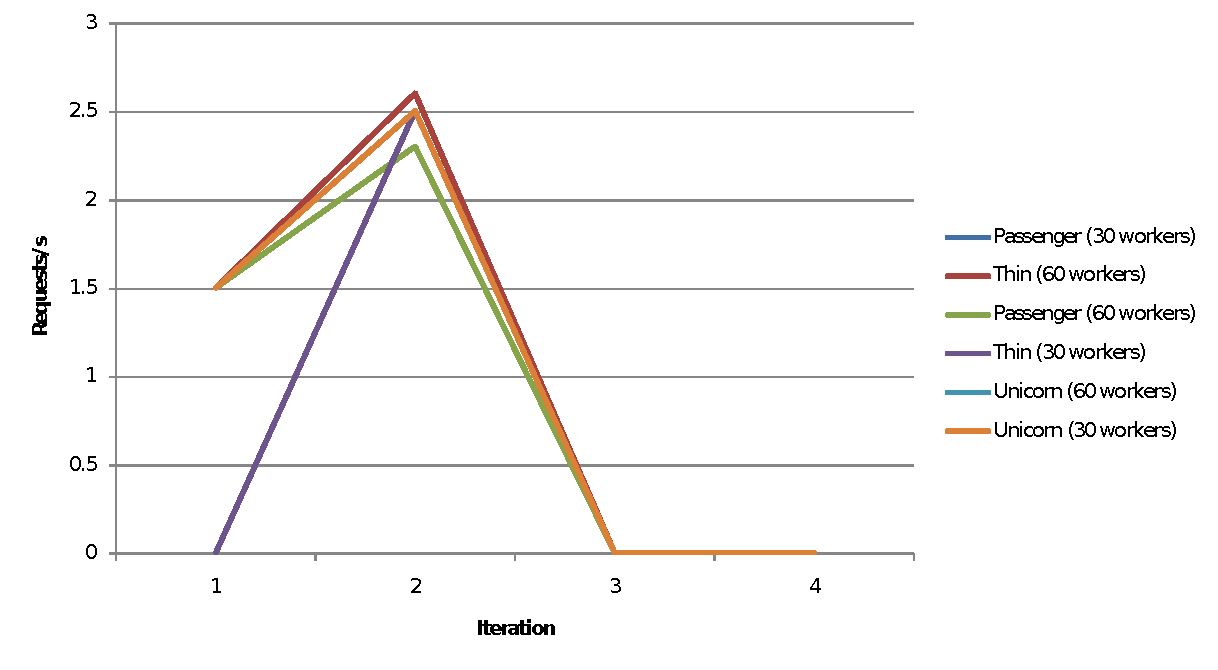
\includegraphics[width=0.95\textwidth]{results_autobench_replies_homepage_ruby18}
  \label{fig:page1_autobench_ruby18_results}
\end{figure}

The test tool, \textit{autobench}, was unable to find a stable request rate on this page. All web servers behaved similarly poor. 

As for the regular page with moderate usage of dynamic content---page 2---the results can be found on figure~\ref{fig:page2_autobench_ruby18_results}.
\begin{figure}[h!]
  \centering
    \caption{Autobench Results on Page 2 (Ruby 1.8)}
    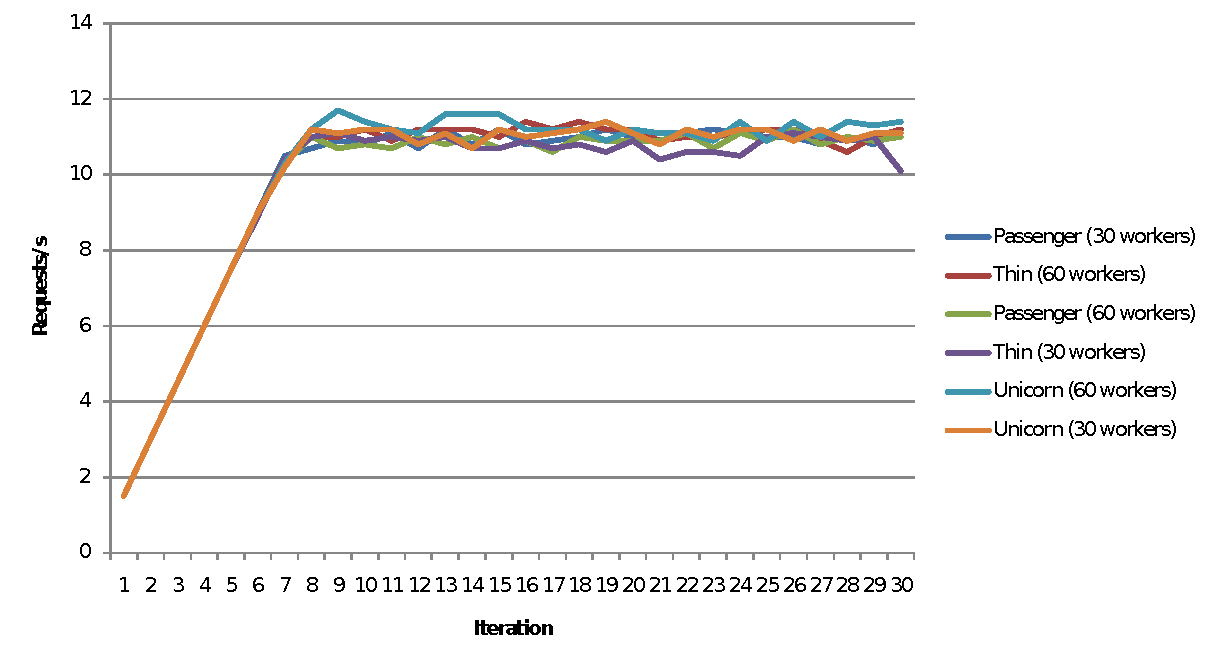
\includegraphics[width=0.95\textwidth]{results_autobench_replies_portal_ruby18}
  \label{fig:page2_autobench_ruby18_results}
\end{figure}

On this test all web servers were able to consistently serve requests, stabilizing at a rate of 10-12 requests per second. Although all had very similar performances, Unicorn with 60 workers consistently yielded slightly better results.

Finally, as for the complex but small API request---page 3---the results are exhibited on figure~\ref{fig:page3_autobench_ruby18_results}.
\begin{figure}[h!]
  \centering
    \caption{Autobench Results on Page 3 (Ruby 1.8)}
    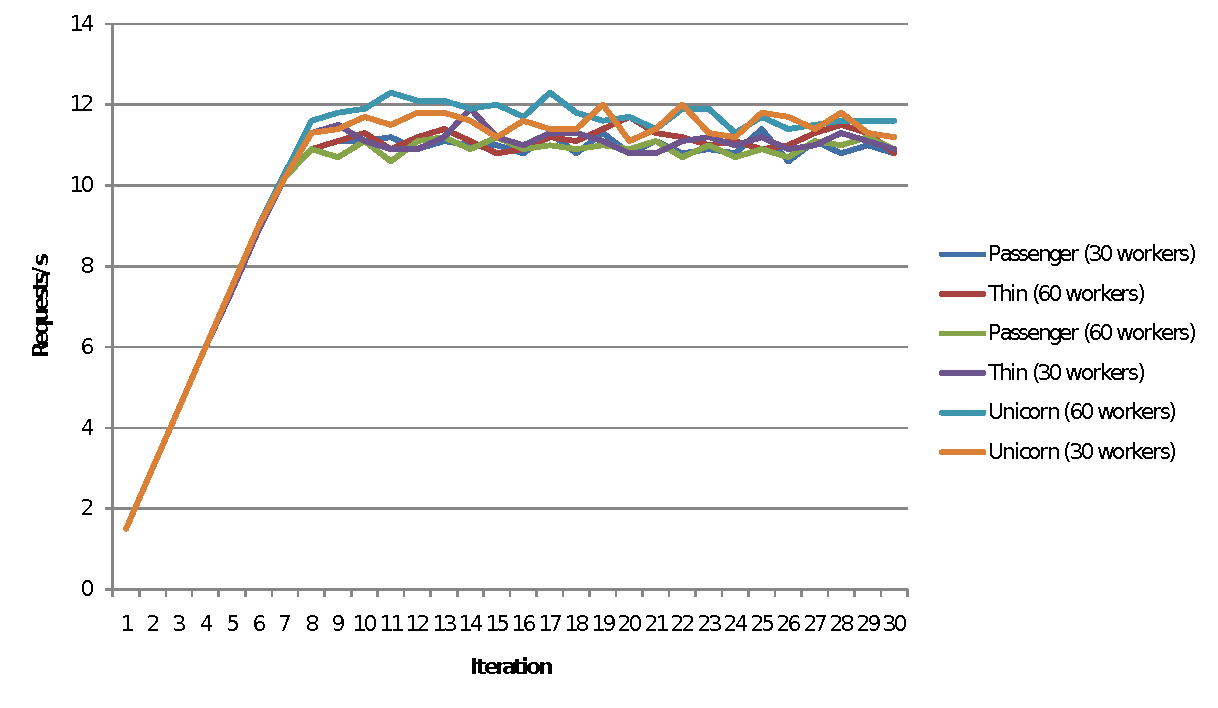
\includegraphics[width=0.95\textwidth]{results_autobench_replies_publication_ruby18}
  \label{fig:page3_autobench_ruby18_results}
\end{figure}

Once again, all web servers were able to maintain a solid request rate, which was stable around 10-13. Unicorn, both with 30 and 60 workers, seems to have a slight performance advantage over its competitors.

The second round was made using Ruby 1.9 on exactly the same pages. The results for the heavy page filled with dynamic content---page 1---can be seen on figure~\ref{fig:page1_autobench_ruby19_results}.
\begin{figure}[h!]
  \centering
    \caption{Autobench Results on Page 1 (Ruby 1.9)}
    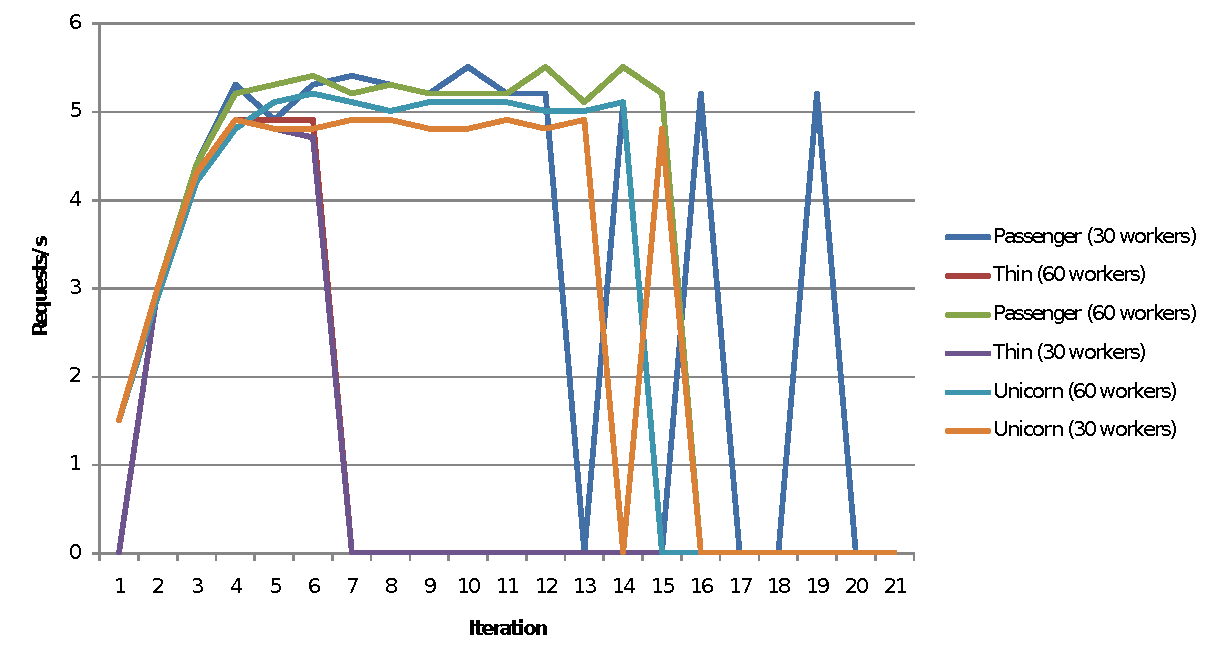
\includegraphics[width=0.95\textwidth]{results_autobench_replies_homepage_ruby19}
  \label{fig:page1_autobench_ruby19_results}
\end{figure}

All web servers have shown extreme improvements after switching to Ruby 1.9 on this page. Most of them were stable through 15-16 iterations instead of a single one and the response rate increased from 2,5 to 4,5-5,5. Thin is the most notable exception, loosing stability after 6 iterations. However, it still represents a remarkable improvement over the previous tests with Ruby 1.8.

As for the regular page with moderate usage of dynamic content---page 2---the results are presented on figure~\ref{fig:page2_autobench_ruby19_results}.
\begin{figure}[h!]
  \centering
    \caption{Autobench Results on Page 2 (Ruby 1.9)}
    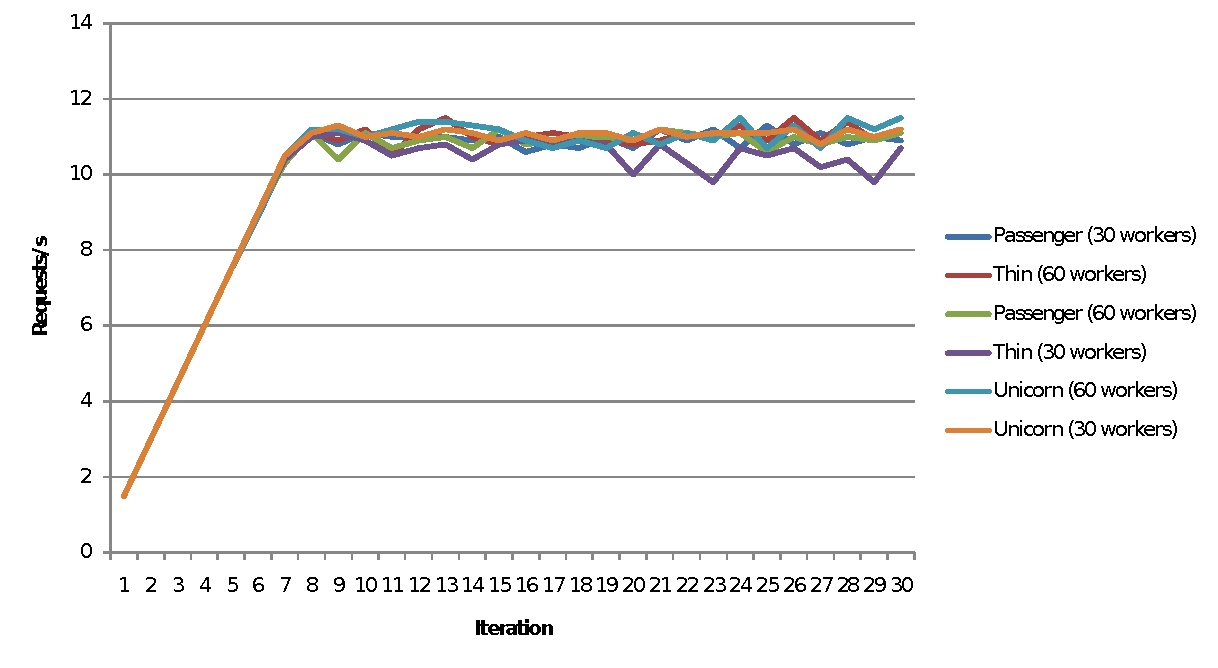
\includegraphics[width=0.95\textwidth]{results_autobench_replies_portal_ruby19}
  \label{fig:page2_autobench_ruby19_results}
\end{figure}

All web servers performed similarly on this test. The results were also very similar to the same test with Ruby 1.8, mainly due to the fact that this page is relatively light on Ruby code.

Finally, as for the complex but small API request---page 3---the results can be found on figure~\ref{fig:page3_autobench_ruby19_results}.
\begin{figure}[h!]
  \centering
    \caption{Autobench Results on Page 3 (Ruby 1.9)}
    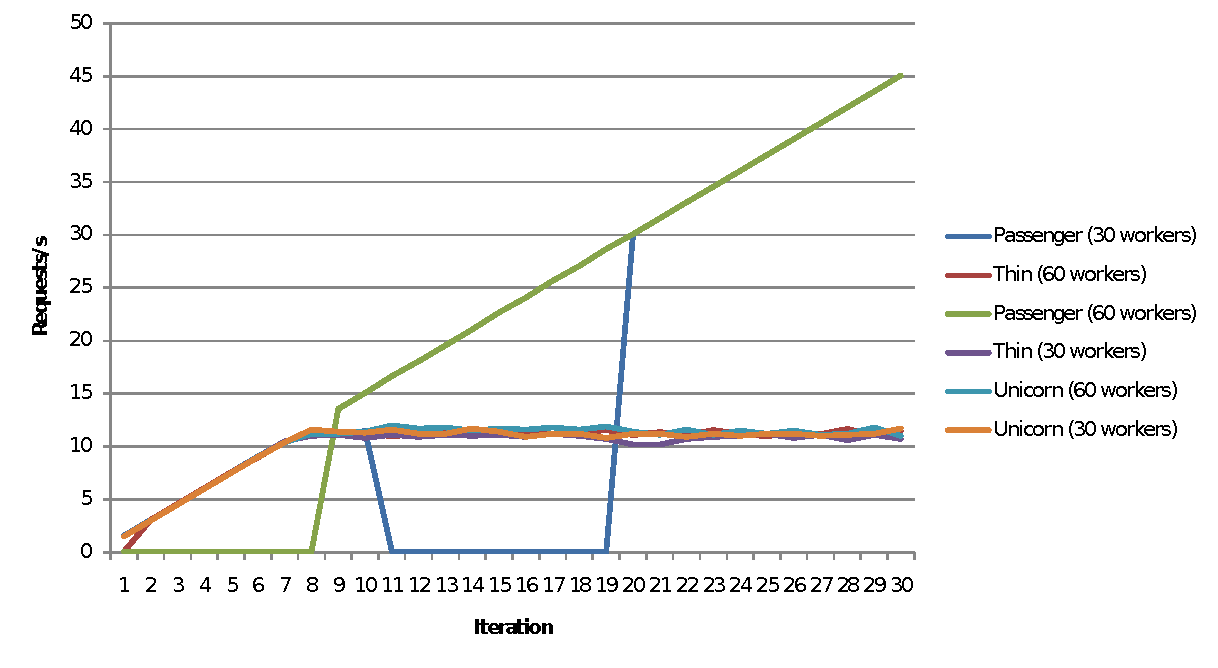
\includegraphics[width=0.95\textwidth]{results_autobench_replies_publication_ruby19}
  \label{fig:page3_autobench_ruby19_results}
\end{figure}

Once again, the results are very similar to those found on the same test with Ruby 1.8. Passenger's behavior is not consistent because its application handler segmentation faults on this specific test---complex API call on Ruby 1.9 with 30 and 60 workers---which is possibly related with shared resource access among workers.

Table~\ref{tab:web_server_memory_usage} exhibits the average memory usage throughout the test. A few conclusions can drawn from the memory usage data. Firstly, Thin always uses less memory than the other web servers. Passenger's memory usage with 30 workers is similar to when it is using 60 workers, which is very high when compared to the others. Finally, using Ruby 1.9 generally causes web servers to use less memory.
\begin{table}[h!t]
  \centering
  \caption{Web Server Memory Usage}
  \label{tab:web_server_memory_usage}
  
  \begin{tabular}{l|c|c|c|c|c|c}

     & \multicolumn{2}{c|}{\textbf{\textsc{Page 1}}} & \multicolumn{2}{c|}{\textbf{\textsc{Page 2}}} & \multicolumn{2}{c}{\textbf{\textsc{Page 3}}} \\ \hline
     & \textbf{Ruby 1.8} & \textbf{Ruby 1.9} & \textbf{Ruby 1.8} & \textbf{Ruby 1.9} & \textbf{Ruby 1.8} & \textbf{Ruby 1.9} \\ \hline
    \textbf{Thin (30)} & 3041 & 2868 & 3018 & 2802 & 2984 & 2849 \\ \hline
    \textbf{Unicorn (30)} & 3463 & 3556 & 3461 & 3354 & 3461 & 3442 \\ \hline
    \textbf{Passenger (30)} & 7794 & 6920 & 7661 & 6650 & 7666 & 6486 \\ \hline
    \textbf{Thin (60)} & 7214 & 6721 & 6993 & 6206 & 6995 & 6488 \\ \hline
    \textbf{Unicorn (60)} & 6808 & 6878 & 6804 & 6566 & 6803 & 6684 \\ \hline
    \textbf{Passenger (60)} & 7798 & 6921 & 7771 & 6687 & 7771 & 8045 \\
  \end{tabular}
\end{table}

After an exhaustive analysis of web servers performance, scalability and memory usage, one can conclude that the differences between web server performance are very small. The area of more impact is memory usage where Thin yields the best results, closely followed by Unicorn. Using Ruby 1.9, however, induces a significant improvement in the results regarding the response rate ability and the stability of all web servers. This difference is clearly noticeable in the heaviest test of the benchmark, where most web servers have shown a $\pm$200\% increase in the request rate and $\pm$1500\% increase in successfully completed iterations.

Most of the tests have shown small to no improvements when doubling the number of workers from 30 to 60. The main bottleneck is related to the nonexistence of a memory object caching system, so increasing the workers had no effect on performance. In fact, the difference between the results of this benchmark and the previously shown ones, with only 4 workers, is remarkably small. Database caching should be in use to precisely determine the difference between having 30 and 60 workers on the aforementioned dual-core machine.

\subsection{Tweaking}
Tweaking a web server's configuration is important to fine-tune its performance. All the examined components are highly configurable and changing some settings can provoke a positive or negative impact in performance.

Apache supports two completely different MPM models. A prefork MPM, which forks a number of identical Apache processes and a worker MPM, which creates multiple threads. The prefork model is generally more effective on systems with one or two processing units where the operating systems is better geared toward time slicing between multiple processes. When more CPUs are available, the worker model will probably be more effective. There are also important settings to address like, for instance, defining the maximum simultaneous connections that Apache can handle using \text{MaxClients} and setting the minimum and maximum number of spare threads/processes.

Unlike Apache, Nginx does not rely on threads nor processes to handle requests. Using a philosophy very similar to Thin's, it aims at solving the C10K problem~\footnote{\url{http://www.kegel.com/c10k.html}} by using an event-driven asynchronous architecture. Nginx supports various event models for handling connections which are optimized for certain situations or operating systems. The user must be certain that it is using the correct one for his system. One of the most efficient models---\textit{epool}---is only supported on Linux systems running a kernel in at least version 2.6, for instance.

Similarly to Apache's worker MPM, Cherokee is a threaded web server. However, it relies on the operating system for request queuing so it also supports many polling methods which are optimized for some systems, like \textit{epoll}. The amount of threads can and should also be configured specifically for each application and machine.

Thin itself is not as configurable as the previously mentioned web servers. However, there are important settings like, for instance, the maximum number of connections, that can be fine-tuned. As mentioned on section~\ref{tech:sec:rails_webservers}, Thin recently became capable of operating in a threaded manner by having a background pool of threads, despite its ``single process single thread'' philosophy. The following section will present a benchmark on this option.

Passenger has a significant amount of configuration options. One of the most important of them all is the process spawning method. While setting it to ``smart'' yields the best results according to its development team, it can cause incompatibilities with some \textit{gems}. The developers must test each system and see if this spawning method is suitable or not. Other interesting options include the number of requests interval in which an application process is restarted, useful for when an application has memory leaks.

Unicorn is a very configurable web server. Its configuration is written in Ruby and there is the possibility to hook into many parts of the start and execution processes. Among all options, there is one that is particularly interesting since it can change the size of the buffers which send and receive TCP data. These can be configured to match the kernel ones---defined by \textit{sysctl}---for optimal performance.

\subsubsection{Thin Performance with Threading Enabled}
Thin recently started to offer the an option which, when activated, will cause requests to be dispatched in a background pool of 20 threads. This slightly contradicts its initial ``single process single thread'' philosophy, though it still relies on an asynchronous event loop for each thread.

A benchmark comparing Thin's performance when threading is enabled or disabled was made using the three previously mentioned pages. Four workers were used in each test and, like the initial benchmarks, \textit{ab} as used to conduct each test. The results are exhibited on table~\ref{tab:thin_threaded_benchmark}.

\begin{table}[h!t]
  \centering
  \caption{Thin with Threading Benchmark Results}
  \label{tab:thin_threaded_benchmark}
  
  \begin{tabular}{c|c|c|c|c|c}

    \textbf{Req. / Conc.} & \textbf{Page} & \textbf{Web Server} & \textbf{Requests/s (\#)} & \textbf{Total time (s)} & \textbf{Mem. Usage (B)} \\ \hline
    \multirow{6}{*}{50/1} & \multirow{2}{*}{API} & Thin & \textbf{9.24} & \textbf{5.411} & \textbf{121213}\\\cline{3-6}
     &  & Thin(threaded) & 7.5 & 6.665 & 126491\\\cline{2-6}
     & \multirow{2}{*}{Heavy} & Thin & \textbf{1.22} & \textbf{41} & \textbf{121506}\\\cline{3-6}
     &  & Thin(threaded) & 0.91 & 55.221 & 128809\\\cline{2-6}
     & \multirow{2}{*}{Regular} & Thin & \textbf{5.99} & \textbf{8.341} & \textbf{121325}\\\cline{3-6}
     &  & Thin(threaded) & 4.67 & 10.711 & 126954\\\hline
    \multirow{6}{*}{100/10} & \multirow{2}{*}{API} & Thin & \textbf{11.84} & \textbf{8.444} & \textbf{121412}\\\cline{3-6}
     &  & Thin(threaded) & 11.81 & 8.465 & 128097\\\cline{2-6}
     & \multirow{2}{*}{Heavy} & Thin & \textbf{2.25} & \textbf{44.495} & \textbf{121666}\\\cline{3-6}
     &  & Thin(threaded) & 1.84 & 54.468 & 133241\\\cline{2-6}
     & \multirow{2}{*}{Regular} & Thin & \textbf{12.14} & \textbf{8.236} & \textbf{121402}\\\cline{3-6}
     &  & Thin(threaded) & 11.73 & 8.527 & 128709\\\hline
    \multirow{6}{*}{500/50} & \multirow{2}{*}{API} & Thin & \textbf{11.67} & \textbf{42.332} & \textbf{121593}\\\cline{3-6}
     &  & Thin(threaded) & 11.47 & 43.605 & 129938\\\cline{2-6}
     & \multirow{2}{*}{Heavy} & Thin & \textbf{2.37} & \textbf{212.427} & \textbf{125128}\\\cline{3-6}
     &  & Thin(threaded) & FAIL & FAIL & 152066\\\cline{2-6}
     & \multirow{2}{*}{Regular} & Thin & \textbf{12.45} & \textbf{40.173} & \textbf{121625}\\\cline{3-6}
     &  & Thin(threaded) & 11.9 & 42.005 & 130860\\\hline
    \multirow{6}{*}{500/100} & \multirow{2}{*}{API} & Thin & 11.48 & 43.546 & \textbf{121613}\\\cline{3-6}
     &  & Thin(threaded) & \textbf{11.6} & \textbf{43.111} & 130082\\\cline{2-6}
     & \multirow{2}{*}{Heavy} & Thin & \textbf{2.45} & \textbf{203.037} & \textbf{127759}\\\cline{3-6}
     &  & Thin(threaded) & FAIL & FAIL & 139153\\\cline{2-6}
     & \multirow{2}{*}{Regular} & Thin & \textbf{12.54} & \textbf{39.883} & \textbf{121650}\\\cline{3-6}
     &  & Thin(threaded) & 11.68 & 42.818 & 130909\\\hline
    \multirow{6}{*}{2500/500} & \multirow{2}{*}{API} & Thin & FAIL & FAIL & \textbf{122012}\\\cline{3-6}
     &  & Thin(threaded) & FAIL & FAIL & 130558\\\cline{2-6}
     & \multirow{2}{*}{Heavy} & Thin & FAIL & FAIL & \textbf{127524}\\\cline{3-6}
     &  & Thin(threaded) & FAIL & FAIL & 134980\\\cline{2-6}
     & \multirow{2}{*}{Regular} & Thin & FAIL & FAIL & \textbf{122020}\\\cline{3-6}
     &  & Thin(threaded) & FAIL & FAIL & 131290\\
  \end{tabular}
\end{table}

Threaded Thin actually performs worse in these test pages. It uses slightly more memory and generally needs a small amount of extra time to complete each test. Threads have an associated overhead, mainly related to the spawning process and the context switches they provoke. Since Thin is based on a really fast asynchronous loop, it is likely that this processing overhead is, in this case, slowing the web server down overall.

\section{Databases} % (fold)
\label{solution:sec:databases}

Concerning databases, the emerging MySQL Ruby library---\textit{mysql2}---was targeted for improvements.

A database, from Rails' perspective, is all about choice. There are three different natively supported relational databases including SQLite, MySQL and PostreSQL. The community, however, as given third-party support to many alternative relational and non-relational databases including MongoDB, CouchDB, DataMapper, SQL Server and Oracle, to name a few.

The popularity of non-relational databases is increasing among the Rails' community, trading enhanced read and write speeds for higher disk usages and fewer functionalities. However, as mentioned on Section~\ref{tech:sec:databases} most Rails applications rely on relational databases, mainly MySQL. On the other hand, benchmarking PostgreSQL against MySQL was discarded as a worthy task because of what was already exposed in Section~\ref{state:sec:databases}. Finally, adapting \textit{Escolinhas.pt} to a non-relational database for further evaluation would require a significant amount of refactoring and some deep architectural changes, being discarded as a possible approach to this component. For these reasons, MySQL was the chosen database to address in this thesis's context.

Due to the aforementioned Rails-centric perspective and the higher probability of success in the medium term, it was not the database itself that was targeted for improvements but instead a recent, improved Ruby database library---\textit{mysql2}. As mentioned in Section~\ref{state:sec:databases}, this Ruby MySQL library can yield results up to 400\% better than the default library in an optimal situation. However, there are caveats which need to be addressed, as explored in the following section.

Improving \textit{mysql2} was the general goal of the work presented in this section.

\subsection{Development}
As mentioned in Chapter~\ref{cha:problem_statement}, \textit{mysql2} handles the conversion of the data between MySQL types and Ruby objects immediately after fetching each row from the database. Since the conversion itself is done in C, there are significant performance improvements over the current default MySQL library which returns all results as ``strings'', forcing Rails to make the conversions in Ruby. 

There are, however, caveats to the approach used by \textit{mysql2}. Since the type conversion is not lazy casted, there is a possibility that the library is converting unnecessary data. If the developer fetches a significant amount of rows from the database but then only uses a small portion of those rows, the library is likely to have a similar or worse performance than the default library. This happens because unlike \textit{mysql2}, using the default database driver Rails will lazy type cast the ``strings'' it receives, only converting the really necessary data.

Adding lazy type casting to fields in \textit{mysql2} was developed in conjunction with one of the library's core developer, Brian Lopez. The changes are still under the core team's development process. There are many optimizations currently being made and support for some uncommon MySQL data types is still being developed and added. For this reason, the changes are not present in the current public release of this database library and there are also no reliable benchmarks to determine the real improvements over the old version of \textit{mysql2} or other MySQL adapters. However, a patch with the changes which can be applied to the library's source code\footnote{\url{http://github.com/brianmario/mysql2/}} is presented on appendix~\ref{ap:mysql2_patch}.


\subsection{Section Overview}
This section exhibited and explained the work concerning databases. A promising Ruby library for MySQL was improved, by changing its behavior concerning database field casting. Instead of converting all fields from MySQL types to Ruby objects upon fetching, it now lazy type casts them as needed.

Adding lazy type casting to \textit{mysql2} allowed to fulfill the general goal initially stated---this library's worst performing case has been reduced by solving one of its biggest caveats.

\section{Ruby on Rails} % (fold)
\label{solution:sec:ruby_on_rails}
The main focus related with Ruby on Rails itself was to improve the current tools for profiling and benchmarking applications. Motivating the adoption of the soon to be released version of this framework---Rails 3---by the community was also a goal regarding this component. Increasing the community's awareness of this subject was also addressed by publishing an article to a popular magazine and engaging in a summer project---Ruby Summer of Code---with high visibility. Nonetheless, some common pitfalls were also addressed while presenting and benchmarking their solutions.

Improving Rails' profiling tools, motivating the adoption of Rails 3 and increasing the community's awareness of this subject were the general goals of the work presented in this section.


\subsection{Benchmarking}
Rails developers can often incur in some development performance pitfalls which can easily be addressed by using some of Rails' powerful functionalities. This section will cover some of these possible pitfalls, propose solutions and generally assert their performance differences.


\subsubsection{Eager Loading}
Eager loading is a core feature of Ruby on Rails which, in certain situations, can lead to significant performance slowdowns because of its absence or misuse. It allows the developer to specify if and which associations should be loaded up front, being the opposite of lazy loading. A classical example of the usefulness of this feature consists in a blog post with comments in which rendering the post's page will also render its comments. Eager loading allows the developer to specify that the comments should be loaded alongside the post, instructing Rails to only use two database queries---one for the post and another for its comments. If not explicitly specified, Rails will load each comment independently while rendering them. Loading the post and eager loading its comments is illustrated in the following code.
\begin{lstlisting}[xleftmargin=30pt,xrightmargin=30pt]
@posts = Post.find(:all, :include => :comments)
\end{lstlisting}

A simple benchmark was performed on a scaffold blog Rails application. The Rails version in use was 2.3.5. The database in use was MySQL using Ruby's default library. A thousand blog posts were generated automatically, along with two hundred thousand comments randomly associated with blog posts. This benchmark compares the time needed to complete a request which fetches all posts along with their comments. The test was run five times to eliminate circumstantial issues and the best results are shown. The results are exhibited on table~\ref{tab:eager_loading}.
\begin{table}[h!t]
  \centering
  \caption{Eager Loading Benchmark Results}
  \label{tab:eager_loading}
  
  \begin{tabular}{c|c}
  
    \textbf{\textsc{Eager Loading}} & \textbf{\textsc{Time (seconds)}} \\
    \hline
    No & 283 \\ \hline
    Yes & 21 \\
  \end{tabular}
\end{table}

In this extreme example, eager loading the data took $\pm$7\% of the time needed to lazy load the data, which is Rails default behavior. Eager loading can have a significant performance impact, depending on the context, as exemplified.


\subsubsection{Transactions}
Rails wraps every database write and update inside a transaction if not instructed otherwise. This happens because of its before/after filter functionality, which allows developers to hook code before and after certain actions are executed. In these cases, the operation and its filters are wrapped inside a transaction.

There are cases, however, where this behavior is suboptimal. When write/update calls are being executed consecutively---for instance, inside a loop---all database calls will be inside their own transaction. This will incur in significant performance penalties, depending on the amount of database actions. However, Rails allows developers to specify where the transaction should begin and end. The following code exemplifies this statement.
\begin{lstlisting}[xleftmargin=30pt,xrightmargin=30pt]
ActiveRecord::Base.transaction do
  (1..100).each { |i| Number.create(:value => i) }
end
\end{lstlisting}
In this example, instead of using one hundred transactions Rails will only use a single one. Using the same environment from the benchmark in the previous section, a benchmark was conducted on asserting the performance difference in explicitly using a global transaction instead of letting Rails place many small transactions which is, as previously mentioned, its behavior by default. This benchmark consisted in creating posts and associated comments, all with the same content. Two tests were made, the first by creating one hundred posts with twenty comments each and a second one by creating one post with two comments. Results can be seen on table~\ref{tab:transaction}.
\begin{table}[h!t]
  \centering
  \caption{Explicit Transaction Benchmark Results}
  \label{tab:transaction}
  
  \begin{tabular}{c|c|c}
  
    & \textbf{\textsc{Explicit Transaction}} & \textbf{\textsc{Time (milliseconds)}} \\ \hline
    100 posts, 20 comments & No & 76017 \\ \hline
    100 posts, 20 comments & Yes & 5223 \\ \hline
    1 post, 2 comments & No & 176 \\ \hline
    1 post, 2 comments & Yes & 137 \\
  \end{tabular}
\end{table}

Using a global transaction on the heaviest test implied a $\pm$93\% reduction on the time needed to write the data. On the lighter test, however, this reduction was of $\pm$22\%. On consecutive writes and/or updates, using a global transaction can significantly increase the performance of the operation.


\subsubsection{Magic Finders}
Rails has a feature commonly called ``magic finders''. It improves code's readability by allowing the developer to replace some calls with smaller and more readable ones. The following example illustrates this feature, comparing with a regular call.\\\\\\ % FIXME: next page?
\begin{lstlisting}[xleftmargin=30pt,xrightmargin=30pt]
Comment.find(:first, :conditions => ["created_at = ?", "2009-11-06 18:25:48"]) # normal find

Comment.find_by_created_at("2009-11-06 18:25:48") # magic find
\end{lstlisting}
These calls, however, have an associated performance penalty. Using the same test environment found on the previous benchmarks, both previously presented calls were benchmarked. The results are presented on table~\ref{tab:magic_finders}.
\begin{table}[h!t]
  \centering
  \caption{Magic Finders Benchmark Results}
  \label{tab:magic_finders}
  
  \begin{tabular}{c|c}
  
    \textbf{\textsc{Type}} & \textbf{\textsc{Time (milliseconds)}} \\ \hline
    Normal find & 62 \\ \hline
    Magic find & 197 \\
  \end{tabular}
\end{table}

The normal find only takes $\pm$32\% of the time needed by the magic find to complete. Since there is a readability/performance trade-off, using either syntaxes is a decision which depends on the project and its developers. The general performance penalty associated with the commonly used magic finders is, however, significant and should be taken into account.


\subsubsection{Fetching Large Groups of Records}
In certain situations, Rails applications need to fetch a significant amount of rows from the database, instantiate each model object and render them in a view. Using the ``find'' helper, this operation can be significantly heavy on memory, as it fetches and loads all records into Ruby objects, and will lock the application until all operations are complete.

However, when Rails 2.3 was introduced it bundled a couple of methods which are likely to be very useful in these situations: ``find\_each'' and ``find\_in\_batches''. The first will retrieve a specified amount of objects at a time, letting the code iterate over the records as if it was a normal ``find'' call. The second is very similar, except that it gives control back to the application every time it fetches a batch. Both methods have a ``batch\_size'' option which defaults to one thousand records. These additional methods have the advantage of using less memory and, as explored in Section~\ref{state:sec:ruby}, less memory usage will trigger Ruby's garbage collector less often, providing better execution times. Notwithstanding these advantages, these methods are unlikely to yield performance improvements when fetching small amounts of records.

To accurately determine the performance benefits involved with switching the ``find'' call with ``find\_each'' when there is a significant amount of records involved, a benchmark was done. The environment was the same as previous benchmarks. The test itself consisted in fetching the two hundred thousand comments in the example blog application. The results can be found on table~\ref{tab:fetch_in_batches}.
\begin{table}[h!t]
  \centering
  \caption{Fetching Records in Batches Benchmark Results}
  \label{tab:fetch_in_batches}
  
  \begin{tabular}{c|c|c}
  
    \textbf{\textsc{Method}} & \textbf{\textsc{Time (seconds)}} & \textbf{\textsc{Memory Usage (MB)}} \\ \hline
    find & 211 & 158 \\ \hline
    find\_each & 195 & 118 \\
  \end{tabular}
\end{table}

Using the alternative method to fetch records in batches, the application needed 10\% less time to fetch the records and used 25\% less memory. These are significant improvements, mainly in memory usage.

\subsection{Development}
The development phase regarding this component involved many distinct activities. First of all, it was crucial to refactor Rails' native profiling and benchmarking tools. Taking into consideration that the release of the new version of the Ruby on Rails framework is nearing, it was important to motivate its early adoption by porting some widely used plugins/gems and one of this framework's most famous applications to the most recent version. After that, a small task related to adding support for the Nginx's \textit{X-Accel-Redirect} header to Rails was performed. Finally, an overview on the current work under the Ruby Summer of Code program is given.


\subsubsection{Refactoring Rails Profiling/Benchmarking Tools}
Rails' profiling and benchmarking tools were nonfunctional on YARV, as they relied on Rub 1.8's now outdated architecture. Ruby evolved very fast and these tools did not keep up, becoming deprecated and useless when used on this version.

Adding Ruby 1.9  support to these tools was crucial, since developers could not rely on the native tools when benchmarking and profiling their applications. By taking advantage of the enhances made to Ruby's profiling tools mentioned in Section~\ref{solution:sec:ruby}, Rails was overhauled~\footnote{\url{http://github.com/rails/rails/commits/master?author=goncalossilva}} and now fully supports profiling and benchmarking under Ruby 1.9.


\subsubsection{Porting Plugins to Rails 3}
Rails 3 adoption by developers is highly conditioned by plugin availability. As mentioned in Section~\ref{tech:sec:ruby_on_rails}, there is a significant amount of plugins available for Ruby on Rails. However, due to the recent Rails' architectural changes, authors generally need to update their plugins/gems to be compatible to this version. The lack of available plugins will certainly limit the adoption rate of this version. In order to help alleviating this problem, some famous plugins were updated to comply with the new Rails API for plugins/gems. All plugins used by \textit{Escolinhas.pt} were analyzed and the ones with the higher watcher count\footnote{GitHub allows users to start ``watching'' repositories, being notified of all changes made to the projects they ``watch''} on their public repositories, were selected. Their names and functionality are:
\begin{description}
  \item[acts\_as\_list,] a plugin for sorting and reordering a number of objects in a list\footnote{\url{http://github.com/goncalossilva/acts_as_list/}};
  \item[permalink\_fu,] a plugin for creating URL-friendly permanent links from object attributes\footnote{\url{http://github.com/goncalossilva/permalink_fu/}};
  \item[acts\_as\_paranoid,] a plugin for hiding records instead of deleting them, being able to recover them\footnote{\url{http://github.com/goncalossilva/rails3_acts_as_paranoid/}}.
\end{description}
All the mentioned plugins were refactored to use the new plugin API. Some tests also needed refactoring, as they used deprecated Rails code. However, updating \textit{permalink\_fu} also involved replacing its character conversion engine since it relied on deprecated Ruby 1.8 functionality, meaning this plugin was not compatible with Ruby's most recent version. On the other hand, \textit{acts\_as\_paranoid} had to be completely rewritten. It was initially developed for Rails 1 and slightly patched to work on Rails 2, having a deprecated architecture which was incompatible with Rails 3. Recreating this plugin from ground up with Rails 3 in mind allowed a $\pm$70\% reduction in lines of code.


\subsubsection{Porting Redmine to Rails 3}
Redmine\footnote{\url{http://www.redmine.org/}} is an open-source flexible project management web application written in Ruby on Rails, created by Jean-Philippe Lang. It is one of the most famous open-source Rails projects, having more than 90 reported major installations worldwide~\cite{redmine_installations}, including the development teams of Ruby, phpBB and Lighttpd. It is a complex platform with over 60 models and 65000 lines of code.

Redmine was upgraded to be compatible with Rails 3 and the source code is hosted at GitHub\footnote{\url{http://github.com/goncalossilva/redmine}}. This upgrade increased Rails 3's visibility while showing the potential performance improvements in upgrading, since this version is reportedly faster. The benefits can be experienced by the users themselves while using Redmine. Many issues had to be addressed, including fixes on the application initialization process, string handling, parameter filtering, plugin support, usage of Javascript helpers and method overriding, among others. All changes can be explored in detail on the project's commit log at GitHub.


\subsubsection{Adding X-Accel-Redirect Support to Rails}
Rails lacks support for Nginx's \textit{X-Accel-Redirect} header by default, so a plugin to add it was developed\footnote{\url{http://github.com/goncalossilva/X-Accel-Redirect}}. Similar to Apache's \textit{X-Sendfile}, \textit{X-Accel-Redirect} can be useful when a user requests the download of a file from the server. If this flag is set on the response body, it will instruct Nginx to handle the file delivery itself. This way, the Rails process will be free to handle other requests instead of blocking to serve the file, delegating that task to Nginx.


\subsubsection{Benchmarking Continuous Integration}
Late in this project's course, applications for the Ruby Summer of Code\footnote{\url{http://www.rubysoc.org/}} began. This program is similar to Google Summer of Code, being a student internship program designed to help fund student development of Ruby-related projects during the summer.

The decision to apply for this program was made, by proposing the development of a Benchmarking Continuous Integration for Ruby on Rails. This proposal was later accepted and a project mentor assigned---Yehuda Katz. Yehuda, the lead developer of the discontinued Merb framework, is one of the most prominent developers behind Rails 3, having joined the core team as soon as the decision to merge Rails and Merb became official.

``Project \#8: Benchmarking CI\footnote{\url{http://www.rubysoc.org/projects/}}'' consists in building an official full-stack benchmarking suite for Ruby on Rails. This way, each commit to the Rails repository will automatically trigger a process where a remote machine starts a new server, runs the tests and reports back the results. As time goes by, it will be possible to watch the evolution of the framework's performance and developers will be able to keep track of the impact their changes have. Any performance regressions will be detected and the responsible developers notified. In its most basic form, it will bring a kind of performance-oriented continuous integration for the Ruby on Rails framework.

The whole Rails community will benefit from having an official benchmarking suite for Ruby on Rails. On one hand, developers will have increased awareness of the framework's performance. They will be able to benchmark their changes and understand their impact on every component, making small adjustments if any significant performance regressions are found. On the other hand, the community will also benefit since Rails will definitely become faster and more scalable over time.


\subsection{Community Blog}
Soon after the start of the project, a public blog named ``Snap Rails''\footnote{\url{http://snaprails.tumblr.com}} was created. Many of the findings done throughout this project have been presented there. Despite being fairly recent, it already surpasses a thousand unique visitors. A map overlay showing their locations is shown on figure~\ref{fig:snaprails_map_overlay}.
\begin{figure}[h!t]
  \centering
    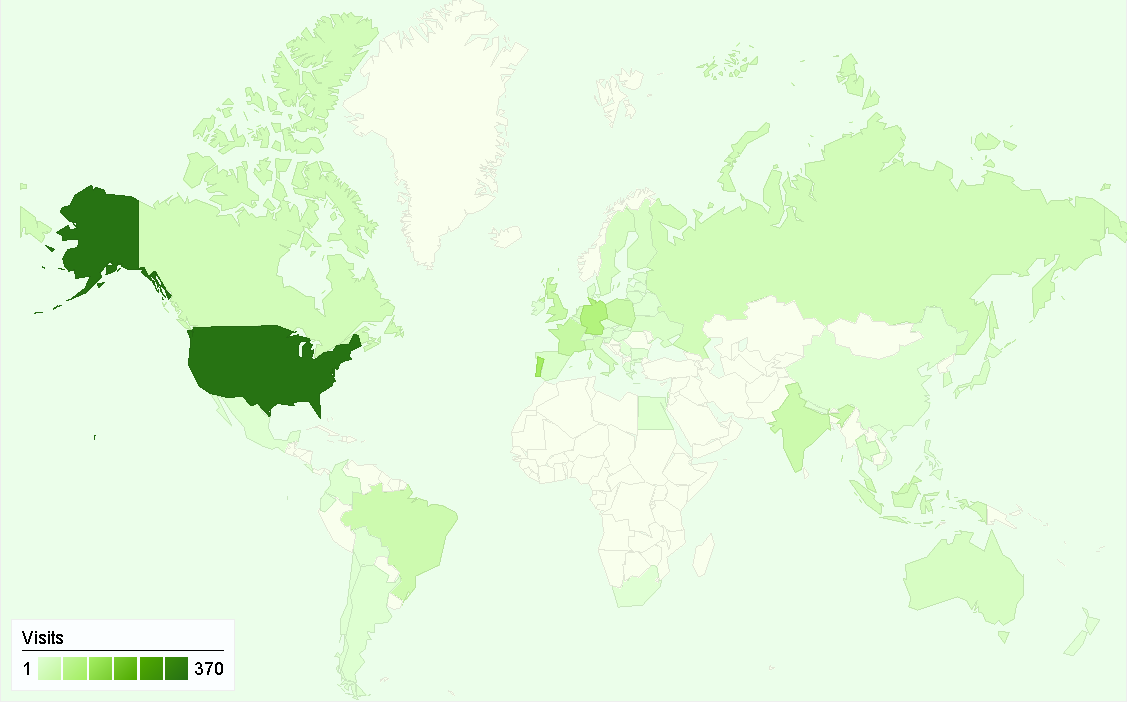
\includegraphics[width=0.75\textwidth]{snaprails_map_overlay}
    \caption{``Snap Rails'' Map Overlay} \label{fig:snaprails_map_overlay}
\end{figure}
Visitor analysis was made using Google Analytics\footnote{\url{http://analytics.google.com}}. With visitors from more than fifty five countries, this blog's purpose is to continuously increase this subject's visibility.


\subsection{Performance-oriented Article Series}
A series of performance-oriented articles for the \textit{Rails Magazine} has also begun. The first article is already present on the sixth edition of the magazine~\cite{rails_magazine_6}, with more to follow on future releases. Similarly to this thesis, this article performance series will cover all system's components, having already started with an introduction to this subject. A copy is exhibited in appendix~\ref{ap:rails_magazine}.

Publishing articles on this matter on such a popular magazine increases this subjects' visibility and the importance in building highly scalable Ruby on Rails applications, possibly igniting the community's awareness of this subject.


\subsection{Section Overview}
This section exhibited and explained the work concerning Ruby on Rails. Regarding benchmarking, common performance pitfalls and their solutions were analyzed. Concerning development, Rails' profiling and benchmarking tools were revamped and now seamlessly integrate with Ruby's. After that, some renowned plugins and Redmine were ported to Rails 3. A plugin which adds support for Nginx's \textit{X-Accel-Redirect} was also created. Finally, a project related to the creation of a performance-oriented continuous integration for Rails under the Ruby Summer of Code program was detailed. This section also presents some work that does not fit under the usual fields---benchmarking, development and tweaking---which is related with increasing the community's awareness of the importance of building highly performant Rails applications. This work is related with the creation of a community blog on this subject and the start of a performance-oriented series of articles for \textit{Rails Magazine}.

Making Rails' profiling tools agnostic to which Ruby version is using them and consequently seamless integrate with YARV allowed to improve these tools. Porting Redmine and various plugins to Rails 3 increased this version's visibility and eased the process of upgrading, motivating its adoption. Creating the general guidelines by using information from this and previous sections, starting a community blog and writing an article series are likely to increase the community's awareness of this subject. Finally, building a benchmarking continuous integration for Rails itself will also increase its developer's awareness of this subject, completing the last of the general goals initially stated.


\begin{comment}
\section*{} % (fold)
The proposed approach consists in envisioning scaling and performance optimization as a whole, where all components take part in scaling and improving the system. Having that said, it is necessary to look out for sensitive dependencies, or the aforementioned \textit{butterfly effect} when optimizing the system.

As an example, the Ruby MRI interpreter's garbage collector consists in an implementation of the \textit{mark-and-sweep} algorithm which is good enough for most applications but lacks the efficiency to deal with heavy and memory intensive applications like Rails~\cite{passenger_whatis}. It is a perfectly reliable garbage collector for the majority of Ruby applications, but it is not the best choice for Rails itself.

Every component must be seen from the Rails perspective and bottlenecks must be identified and contoured.

To achieve this, we need to set up an initial setup for benchmarking, tweaking and patching. This involves using a specific operating system and that choice will be made based on three essential factors:
\begin{enumerate}
  \item The information gathered in the state of the art of Operating Systems, from the Rails perspective;
  \item A small set of benchmarks for standard performance analysis;
  \item Configuration easiness, as some operating systems and distributions tend to stimulate system tweaking by allowing easy access to certain features and configurations and others, on the other hand, might not have this feature in their goals and consequently make it harder to tweak and configure at will.
\end{enumerate}
After starting with the chosen operating system, kernel settings will fill the first chapter of the abovementioned guidelines as they have a great impact on operating system behavior. Important settings regarding TCP/IP behavior, I/O scheduler, Preemption, Interrupt Timers \textit{et al.} must be tested and benchmarked from the Rails perspective in order to achieve a configuration set that suits Rails --- and all the other components --- best.

When the mentioned set of configurations and settings is met, the web servers will become the research and development target. Not all of them will be tested since the state of the art on web servers rules some of them out, but at least two will be taken into a small set of benchmarks and configuration tweaking. After finding which suits Rails best, research will deepen and eventual bottlenecks might be found and improving patches will be developed.

Following the web server choice, ruby interpreters will become the aim. Once again, the state of the art on ruby interpreters rules some of them out but at least two will endure a small set of benchmarks and configuration tweaking to conclude which scales better and has a better performance from the Rails point of view. Possible bottlenecks will be found and, once again, an attempt at solving the most critical ones will be made. After that, a series of patches will be released in order to improve that interpreter even further.

The next target is a commonly know bottleneck on web applications – the database. A few will be tested, following the \textit{at least two} rule, but here there is a clear division on two essential types of databases:
\begin{enumerate}
  \item Schema-based databases, like the famous MySQL or PostgreSQL;
  \item Schema-free document-oriented databases, like MongoDB or CouchDB.
\end{enumerate}
While schema-based databases are very popular and reliable, not to mention that they are tested thoroughly because of being so popular and so mature, schema-free databases emerge as high performance solutions with little pitfalls. Both types must be tested and benchmarked, in order to provide results and configurations that suit most Rails applications, whether they are using a schema-based database or not. Bottlenecks will also be searched and attempts at fixing them will be made. An approach to caching will also be made in the database regard, as it is a crucial concept when scaling. If major bottlenecks are found in the existing caching solutions, an improvement attempt will be made and possible positive outcomes will be submitted as patches to the developing community.

The next phase is related to Rails itself. Since, as mentioned, Rails 3.0 is a big improvement over Rails 2.3 from a performance perspective, no attempts at improving Rails 2.3 will be made. However, remaining bottlenecks in Rails 3.0 will be targeted for improvement with guidance from the Rails core development team.
Finally, the case-study application, Escolinhas~\cite{escolinhas}, will be aimed for improvement. The architecture and code will be reviewed to find and erase performance bottlenecks, always taking Rails' strengths and weaknesses into account to fully optimize the application for the framework it is being developed on. This will allow the development of a small set of generalist guidelines and programming conventions that suit most Rails developers and their respective applications.
Different components become the main focus at different times. A brief summary of the above information is presented in table~\ref{tab:research_development_schedule} which indicates when a given component will become the main focus and for how long that is expected to happen.
\begin{table}[h]
  \centering
  \begin{tabular}{p{8cm}|p{2.1cm}p{3.5cm}}
    \textsc{Target component}
  & \textsc{Start date}
  & \textsc{Duration (weeks)}
  \\
  \hline
    \textbf{OS Choosing}
  & 15/02/2010
  & 1
  \\
  \hline
    \textbf{OS kernel testing and tunning}
  & 22/02/2010
  & 1
  \\
  \hline
    \textbf{Web server testing and bottleneck research}
  & 01/03/2010
  & 1
  \\
  \hline
    \textbf{Web server bottleneck improvements}
  & 08/03/2010
  & 1
  \\
  \hline
    \textbf{Ruby interpreter testing and bottleneck research}
  & 15/03/2010
  & 1
  \\
  \hline
    \textbf{Ruby interpreter bottleneck improvements}
  & 22/03/2010
  & 1.5
  \\
  \hline
    \textbf{DB testing and bottleneck research}
  & 31/03/2010
  & 1
  \\
  \hline
    \textbf{DB bottleneck improvements}
  & 07/04/2010
  & 1
  \\
  \hline
    \textbf{Rails 3.0 bottleneck research}
  & 14/04/2010
  & 1
  \\
  \hline
    \textbf{Rails 3.0 bottleneck improvements}
  & 21/04/2010
  & 2.5
  \\
  \hline
    \textbf{Escolinhas analysis and bottleneck research}
  & 10/05/2010
  & 1
  \\
  \hline
    \textbf{Escolinhas platform improvements}
  & 17/05/2010
  & 3
  \\
  \hline
    \textbf{Write dissertation report}
  & 07/06/2010
  & 4
  \\
  \end{tabular}  
  \caption{Component focus scheduling}
  \label{tab:research_development_schedule}  
\end{table}\\
In order to benchmark every component, others which run on top of it must be taken into account. This way, the research starts by involving every single component. After having conclusive results for each one of them they will be removed from the research, as shown on figure~\ref{fig:gantt}. The main focus will then leap into another component.
\begin{figure}[th]
  \begin{center}
    \leavevmode
 
    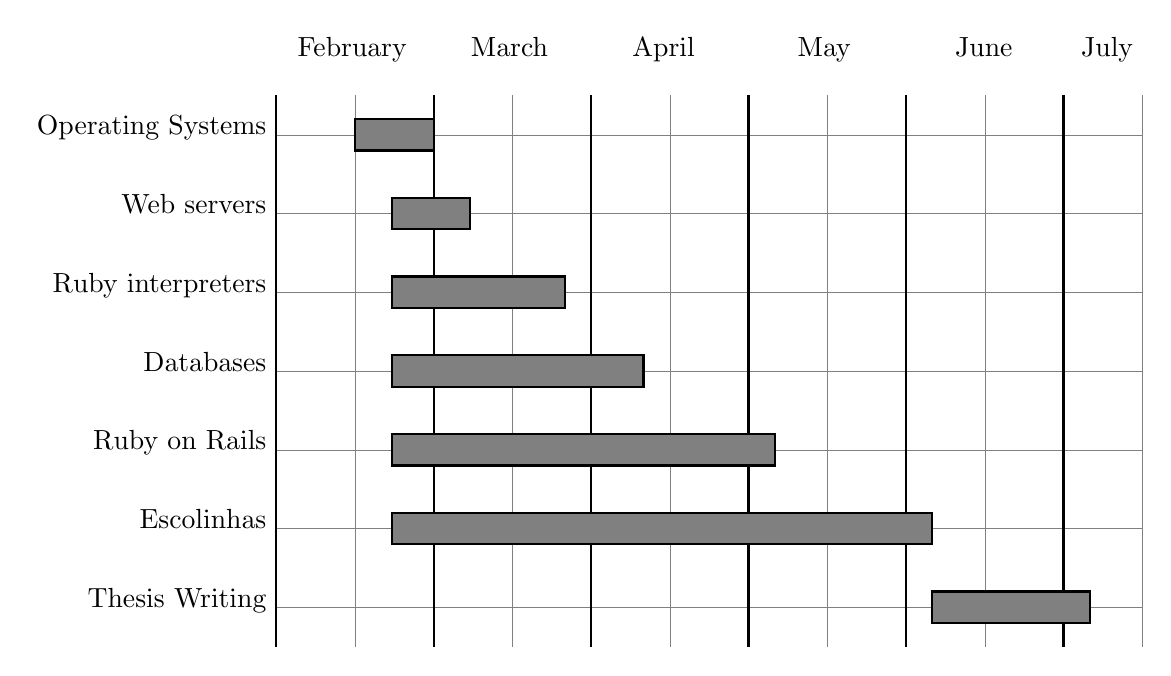
\begin{tikzpicture}[y=-1cm]
      \draw[help lines] (0,7.5) grid (11,0.5);
      \draw[thick] (0,0.5) -- (0,7.5);
      \draw[thick] (2,0.5) -- (2,7.5);
      \draw[thick] (4,0.5) -- (4,7.5);
      \draw[thick] (6,0.5) -- (6,7.5);
      \draw[thick] (8,0.5) -- (8,7.5);
      \draw[thick] (10,0.5) -- (10,7.5);
      
      \node at (0.15,0.0) [anchor=base west] {February};
      \node at (2.35,0.0) [anchor=base west] {March};
      \node at (4.4,0.0) [anchor=base west] {April};
      \node at (6.5,0.0) [anchor=base west] {May};
      \node at (8.5,0.0) [anchor=base west] {June};
      \node at (10.1,0.0) [anchor=base west] {July};
      
      \ganttline{1}{Operating Systems}{15}{30}
      \ganttline{2}{Web servers}{22}{37}
      \ganttline{3}{Ruby interpreters}{22}{55}
      \ganttline{4}{Databases}{22}{70}
      \ganttline{5}{Ruby on Rails}{22}{95}
      \ganttline{6}{Escolinhas}{22}{125}
      \ganttline{7}{Thesis Writing}{125}{155}
    \end{tikzpicture}
 
    \caption{Work scheduling}
    \label{fig:gantt}
  \end{center}
\end{figure}\\
All the mentioned testing, tuning, bottleneck research and improvements are directly related to scaling and performance optimizations, as suggested throughout this thesis.
Once again, it becomes critical to reaffirm that each area will be essentially targeted from the Rails perspective, taking sensitive dependences into account in order to avoid optimizing a specific component while taking the risk of making the system, as a whole, slower or less scalable.
\end{comment}


  %% Conclusions
  \chapter{Conclusions} % (fold)
\label{cha:conclusions}
\headermark{Conclusions}
\section*{} % (fold)

\begin{comment}
This is deprecated!!!!!!

The existing research provides a solid base for future work on this subject. The endured technology overview allowed the creation of an expectancy base for each component. The state of the art provided an overview of the current engaged work on related, if not similar, subjects.

All the gathered and structured information permitted option narrowing when it comes to future work. Taking into account the research and conclusions of some related work, some components will be left out of future benchmarking, tuning, testing and improvement.

On the Operating System's concern, Microsoft's operating system will be left out of future efforts since its Ruby and Rails support is significantly poor and inefficient. The lack of benchmark and testing information about BSD and the fact that its performance should be similar to Linux's include it in the test group. Concluding, the Operating Systems contempt by this project will be Linux and BSD.

Ruby is currently in version 1.9 which has many improvements over the previous version, both performance and not performance-oriented. Since YARV is the only one to support its specification to full extent, this will be the only interpreter targeted for improvements. Luckily, Rubinius' 1.9 support is growing day by day and it is close to 100\%. Only time will tell if this interpreter will be considered as well.

Rails web servers' situation is more flat. Only WEBrick is left out for obvious reasons --- it was Rails' pioneer web server but lacks the efficiency to compete with nowadays alternatives.

When it comes to relational databases, MySQL's scaling and performance capabilities shine. On the other hand, MongoDB presents itself as a worthy alternative but it has an important characteristic --- it is a schema-less database. PostgreSQL, although providing many interesting features, is not efficient enough to compete with MySQL, being left out of the test group for further work. MySQL and MongoDB are targeted for all the aforementioned improvement cycle.

Rails is growing fast and version 3 will soon to be publicly released. It solves many existing performance bottlenecks in Rails 2.3 and improves its predecessor code by a great deal. Working on Rails 2.3 would not be very productive since it will soon become deprecated and inefficient when compared with the most recent version. Version 3 will be the main target focus for further development.

The application itself, \textit{Escolinhas}, would benefit from huge performance gains just by being ported to Ruby 1.9 and Rails 3. The remaining improvements are dependant on the improvement cycles of all the components mentioned before, as performance bottlenecks must be found and solved on each setup.

Ultimately this research provided a careful overview over the involved technologies and their current state, sustaining the creation of a solid research and development plan for future efforts.
\end{comment}

\section{Conclusions}
Guidelines and conventions are created

Escolinhas is more scalable

Open-source contribution with considerable range and big impact


\section{Summary of Contributions}

Created generic guidelines and conventions

Improved Rails profiling abilities

Improved Ruby's profiling abilities

Improved Ruby's GC flexibility

Ported Escolinhas to Ruby 1.9

Ported Redmine to Ruby 1.9 and Rails 3

Ported the plugins used by Escolinhas to Rails 3

Demonstrated Ruby's performance on different OSes

Demonstrated OSes performance with generic and web-oriented benchmarks

Creation of web server benchmarking scripts

In-depth analysis of the current web servers performance

Demonstrated the performance of the latest Ruby against the most used version

Joint of many micro-researches (?)


\section{Future Research}

Research other databases aside mysql

Invest in alternative Ruby interpreters (which should be stable in a near future)

Develop a generational GC for Ruby


  
  
  %%----------------------------------------
  %% Final materials
  %%----------------------------------------

  \begin{singlespace}
    \PrintBib{references}

    %% Index
    %% Uncomment next command if index is required,
    %% don't forget to run ``makeindex mieic'' command
    %\PrintIndex

    %% Comment next 2 commands if numbered appendixes not used
    \appendix
    \chapter{Ruby 1.9 Encoding Patch} % (fold)
\label{ap:ruby19_encoding_patch}

The Ruby patch developed to fix the encoding issues when using non-ASCII characters on version 2.3.5 of Ruby on Rails.\\\\

\begin{lstlisting}[language=ruby]
# coding: UTF-8

# TODO: Most of these issues are not present in Rails 3. Remove this when updating.

# Force mysql rows to be UTF-8 (see rails.lighthouseapp.com/projects/8994/tickets/2476)
require 'mysql'
 
class Mysql::Result
  def encode(value, encoding = "utf-8")
    (String  === value && value.respond_to?(:force_encoding)) ? value.force_encoding(encoding) : value
  end
  
  def each_utf8(&block)
    each_orig do |row|
      yield row.map {|col| encode(col) }
    end
  end
  alias each_orig each
  alias each each_utf8
 
  def each_hash_utf8(&block)
    each_hash_orig do |row|
      row.each {|k, v| row[k] = encode(v) }
      yield(row)
    end
  end
  alias each_hash_orig each_hash
  alias each_hash each_hash_utf8
end

# fix template rendering
module ActionView
  # NOTE: The template that this mixin is being included into is frozen
  # so you cannot set or modify any instance variables
  module Renderable #:nodoc:
    extend ActiveSupport::Memoizable


    private    
    def compile!(render_symbol, local_assigns)
        locals_code = local_assigns.keys.map { |key| "#{key} = local_assigns[:#{key}];" }.join

        source = <<-end_src
          def #{render_symbol}(local_assigns)
            old_output_buffer = output_buffer;#{locals_code};#{compiled_source}
          ensure
            self.output_buffer = old_output_buffer
          end
        end_src
        
        # Workaround for erb
        source.force_encoding('utf-8') if '1.9'.respond_to?(:force_encoding)

        begin
          ActionView::Base::CompiledTemplates.module_eval(source, filename, 0)
        rescue Errno::ENOENT => e
          raise e # Missing template file, re-raise for Base to rescue
        rescue Exception => e # errors from template code
          if logger = defined?(ActionController) && Base.logger
            logger.debug "ERROR: compiling #{render_symbol} RAISED #{e}"
            logger.debug "Function body: #{source}"
            logger.debug "Backtrace: #{e.backtrace.join("\n")}"
          end

          raise ActionView::TemplateError.new(self, {}, e)
        end
      end

  end
end

# the previous fix causes issues in uploaded files encoding, fixed here
module ActionController
  class Request
    private

      # Convert nested Hashs to HashWithIndifferentAccess and replace
      # file upload hashs with UploadedFile objects
      def normalize_parameters(value)
        case value
        when Hash
          if value.has_key?(:tempfile)
            upload = value[:tempfile]
            upload.extend(UploadedFile)
            upload.original_path = value[:filename]
            upload.content_type = value[:type]
            upload
          else
            h = {}
            value.each { |k, v| h[k] = normalize_parameters(v) }
            h.with_indifferent_access
          end
        when Array
          value.map { |e| normalize_parameters(e) }
        else
          value.force_encoding(Encoding::UTF_8) if value.respond_to?(:force_encoding)
          value
        end
      end
  end
end
\end{lstlisting}

    \chapter{Ruby 1.9 Encoding Task} % (fold)
\label{ap:ruby19_encoding_task}

The rake task developed to automatically manage all Ruby files and set their default encoding to UTF-8. It inserts the encoding header when needed and standardizes the variant in use to ``\# coding: UTF-8''.\\\\

\begin{lstlisting}[language=ruby]
desc "Manage the encoding header of Ruby files"
task :check_encoding_headers => :environment do
  files = Array.new
  ["*.rb", "*.rake"].each do |extension|
    files.concat(Dir[ File.join(Dir.getwd.split(/\\/), "**", extension) ])
  end

  files.each do |file|
    content = File.read(file)
    next if content[0..16] == "# coding: UTF-8\n\n"
    
    ["\n\n", "\n"].each do |file_end|
      content = content.gsub(/(# encoding: UTF-8#{file_end})|(# coding: UTF-8#{file_end})|(# -*- coding: UTF-8 -*-#{file_end})/i, "")
    end

    new_file = File.open(file, "w")
    new_file.write("# coding: UTF-8\n\n"+content)
    new_file.close
  end
end

\end{lstlisting}

    \chapter{Ruby 1.9 configuration} % (fold)
\label{ap:ruby19_configuration}

The following command snippet starts the Ruby interpreter with an example configuration on UNIX.\\\\

\begin{lstlisting}[language=bash]
export RUBY_HEAP_SLOTS_INCREMENT=500000
export RUBY_HEAP_MIN_SLOTS=500000
export RUBY_HEAP_SLOTS_GROWTH_FACTOR=1.1
export RUBY_GC_MALLOC_LIMIT=40000000
export RUBY_HEAP_FREE_MIN=100000
ruby
\end{lstlisting}

    \chapter{Ruby-Prof HTML Stack Printer} % (fold)
\label{ap:ruby-prof_html_stack_printer}

A snippet of the HTML output of this graphic hierarchical printer. It contains many information like the relative time elapsed of each call, the number of times a given call occured and even background colors to highlight faster and slower calls, among others.\\\\

\begin{figure}[h]
  \centering
    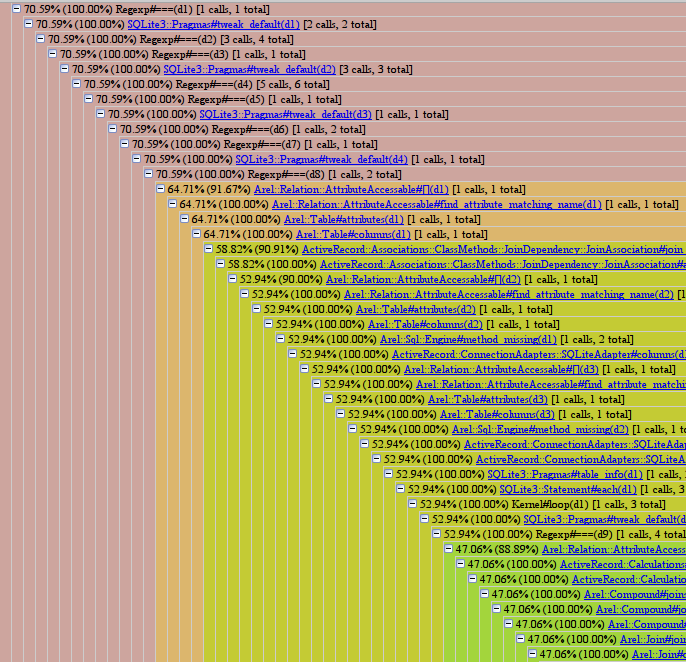
\includegraphics[width=0.9\textwidth]{ruby-prof_html_stack_printer}
    \caption{Ruby-prof HTML Stack Printer} \label{fig:ruby-prof_html_stack_printer}
\end{figure}

    \chapter{Memory usage monitor script} % (fold)
\label{ap:ruby19_encoding_patch}

A small Ruby script that measures the memory usage of specified processes. The user can configure the refresh interval and the output directory. The result is recorded in CSV.\\\\

\begin{lstlisting}
logs = Hash.new
temp_dir = ARGV[0]
delta = ARGV[1].to_f != 0 ? ARGV[1] : 1

while true do
  ARGV[1..-1].each do |arg|
    next if ARGV[1].to_f != 0
    (`pidof #{arg}`.split-logs.keys).each do |pid|
      logs[pid] = File.open("#{temp_dir}/#{(arg.gsub(/[^a-zA-Z 0-9]/, "")).gsub(/\s/,'-')}.#{pid}.csv", "w")
    end
  end

  logs.each do |pid, log|
    begin
      f = File.open("/proc/#{pid}/status", 'r').read
    rescue
      next
    end
    
    begin
      vmpeak = f.match('VmPeak:\s+(\d+)\s+kB')[1]
      vmsize = f.match('VmSize:\s+(\d+)\s+kB')[1]
      vmrss = f.match('VmRSS:\s+(\d+)\s+kB')[1]

      log.write("#{vmpeak},#{vmsize},#{vmrss}\n")
      log.flush
    rescue
      log.close
      logs.delete(pid)
    end
  end
  
  sleep delta.to_i
end
\end{lstlisting}

    \chapter{Lazy Type Casting in mysql2} % (fold)
\label{ap:mysql2_patch}

A patch which enables lazy type casting of fields on of Ruby's \textit{MySQL} database libraries, \textit{mysql2}.\\\\

\begin{lstlisting}
diff --git a/ext/mysql2_ext.c b/ext/mysql2_ext.c
index 3f791d3..fadea7b 100644
--- a/ext/mysql2_ext.c
+++ b/ext/mysql2_ext.c
@@ -370,7 +370,7 @@ static VALUE nogvl_read_query_result(void *ptr)
   return res == 0 ? Qtrue : Qfalse;
 }
 
-/* mysql_store_result may (unlikely) read rows off the socket */
+/*  may (unlikely) read rows off the socket */
 static VALUE nogvl_store_result(void *ptr)
 {
   MYSQL * client = ptr;
@@ -521,92 +521,8 @@ static VALUE rb_mysql_result_fetch_row(int argc, VALUE * argv, VALUE self) {
       }
       rb_ary_store(wrapper->fields, i, field);
     }
-
+    VALUE val = INT2NUM(wrapper->lastRowProcessed+i);
     if (row[i]) {
-      VALUE val;
-      switch(fields[i].type) {
-        case MYSQL_TYPE_NULL:       // NULL-type field
-          val = Qnil;
-          break;
-        case MYSQL_TYPE_BIT:        // BIT field (MySQL 5.0.3 and up)
-          val = rb_str_new(row[i], fieldLengths[i]);
-          break;
-        case MYSQL_TYPE_TINY:       // TINYINT field
-        case MYSQL_TYPE_SHORT:      // SMALLINT field
-        case MYSQL_TYPE_LONG:       // INTEGER field
-        case MYSQL_TYPE_INT24:      // MEDIUMINT field
-        case MYSQL_TYPE_LONGLONG:   // BIGINT field
-        case MYSQL_TYPE_YEAR:       // YEAR field
-          val = rb_cstr2inum(row[i], 10);
-          break;
-        case MYSQL_TYPE_DECIMAL:    // DECIMAL or NUMERIC field
-        case MYSQL_TYPE_NEWDECIMAL: // Precision math DECIMAL or NUMERIC field (MySQL 5.0.3 and up)
-          val = rb_funcall(cBigDecimal, intern_new, 1, rb_str_new(row[i], fieldLengths[i]));
-          break;
-        case MYSQL_TYPE_FLOAT:      // FLOAT field
-        case MYSQL_TYPE_DOUBLE:     // DOUBLE or REAL field
-          val = rb_float_new(strtod(row[i], NULL));
-          break;
-        case MYSQL_TYPE_TIME: {     // TIME field
-          int hour, min, sec, tokens;
-          tokens = sscanf(row[i], "%2d:%2d:%2d", &hour, &min, &sec);
-          val = rb_funcall(rb_cTime, intern_local, 6, INT2NUM(0), INT2NUM(1), INT2NUM(1), INT2NUM(hour), INT2NUM(min), INT2NUM(sec));
-          break;
-        }
-        case MYSQL_TYPE_TIMESTAMP:  // TIMESTAMP field
-        case MYSQL_TYPE_DATETIME: { // DATETIME field
-          int year, month, day, hour, min, sec, tokens;
-          tokens = sscanf(row[i], "%4d-%2d-%2d %2d:%2d:%2d", &year, &month, &day, &hour, &min, &sec);
-          if (year+month+day+hour+min+sec == 0) {
-            val = Qnil;
-          } else {
-            if (month < 1 || day < 1) {
-              rb_raise(cMysql2Error, "Invalid date: %s", row[i]);
-              val = Qnil;
-            } else {
-              val = rb_funcall(rb_cTime, intern_local, 6, INT2NUM(year), INT2NUM(month), INT2NUM(day), INT2NUM(hour), INT2NUM(min), INT2NUM(sec));
-            }
-          }
-          break;
-        }
-        case MYSQL_TYPE_DATE:       // DATE field
-        case MYSQL_TYPE_NEWDATE: {  // Newer const used > 5.0
-          int year, month, day, tokens;
-          tokens = sscanf(row[i], "%4d-%2d-%2d", &year, &month, &day);
-          if (year+month+day == 0) {
-            val = Qnil;
-          } else {
-            if (month < 1 || day < 1) {
-              rb_raise(cMysql2Error, "Invalid date: %s", row[i]);
-              val = Qnil;
-            } else {
-              val = rb_funcall(cDate, intern_new, 3, INT2NUM(year), INT2NUM(month), INT2NUM(day));
-            }
-          }
-          break;
-        }
-        case MYSQL_TYPE_TINY_BLOB:
-        case MYSQL_TYPE_MEDIUM_BLOB:
-        case MYSQL_TYPE_LONG_BLOB:
-        case MYSQL_TYPE_BLOB:
-        case MYSQL_TYPE_VAR_STRING:
-        case MYSQL_TYPE_VARCHAR:
-        case MYSQL_TYPE_STRING:     // CHAR or BINARY field
-        case MYSQL_TYPE_SET:        // SET field
-        case MYSQL_TYPE_ENUM:       // ENUM field
-        case MYSQL_TYPE_GEOMETRY:   // Spatial fielda
-        default:
-          val = rb_str_new(row[i], fieldLengths[i]);
-#ifdef HAVE_RUBY_ENCODING_H
-          // rudimentary check for binary content
-          if ((fields[i].flags & BINARY_FLAG) || fields[i].charsetnr == 63) {
-            rb_enc_associate_index(val, binaryEncoding);
-          } else {
-            rb_enc_associate_index(val, utf8Encoding);
-          }
-#endif
-          break;
-      }
       rb_hash_aset(rowHash, field, val);
     } else {
       rb_hash_aset(rowHash, field, Qnil);
@@ -651,20 +567,20 @@ static VALUE rb_mysql_result_each(int argc, VALUE * argv, VALUE self) {
         wrapper->lastRowProcessed++;
       }
 
-      if (row == Qnil) {
+      /*if (row == Qnil) {
         // we don't need the mysql C dataset around anymore, peace it
         rb_mysql_result_free_result(wrapper);
         return Qnil;
-      }
+      }*/
 
       if (block != Qnil) {
         rb_yield(row);
       }
     }
-    if (wrapper->lastRowProcessed == wrapper->numberOfRows) {
+    /*if (wrapper->lastRowProcessed == wrapper->numberOfRows) {
       // we don't need the mysql C dataset around anymore, peace it
       rb_mysql_result_free_result(wrapper);
-    }
+    }*/
   }
 
   return wrapper->rows;
@@ -686,6 +602,118 @@ static VALUE rb_raise_mysql2_error(MYSQL *client) {
   return Qnil;
 }
 
+static VALUE rb_mysql_result_cast(VALUE self, VALUE index) {
+  mysql2_result_wrapper * wrapper;
+  MYSQL_FIELD * field = NULL;
+  MYSQL_ROW row;
+  VALUE val;
+  unsigned long * fieldLengths;
+  void * ptr;
+  
+  GetMysql2Result(self, wrapper);
+  
+  if (wrapper->numberOfFields == 0) {
+    wrapper->numberOfFields = mysql_num_fields(wrapper->result);
+    wrapper->fields = rb_ary_new2(wrapper->numberOfFields);
+  }
+  
+  unsigned long r = index / wrapper->numberOfRows;
+  int c = index % wrapper->numberOfFields;
+  
+  ptr = wrapper->result;
+  mysql_data_seek(ptr, r); // <--- Segmentation fault
+  row = (MYSQL_ROW)rb_thread_blocking_region(nogvl_fetch_row, ptr, RUBY_UBF_IO, 0);
+  
+  field = mysql_fetch_field_direct(ptr, c);
+  fieldLengths = mysql_fetch_lengths(wrapper->result);
+  
+  switch(field->type) {
+    case MYSQL_TYPE_NULL:       // NULL-type field
+      val = Qnil;
+      break;
+    case MYSQL_TYPE_BIT:        // BIT field (MySQL 5.0.3 and up)
+      val = rb_str_new(row[c], fieldLengths[c]);
+      break;
+    case MYSQL_TYPE_TINY:       // TINYINT field
+    case MYSQL_TYPE_SHORT:      // SMALLINT field
+    case MYSQL_TYPE_LONG:       // INTEGER field
+    case MYSQL_TYPE_INT24:      // MEDIUMINT field
+    case MYSQL_TYPE_LONGLONG:   // BIGINT field
+    case MYSQL_TYPE_YEAR:       // YEAR field
+      val = rb_cstr2inum(row[c], 10);
+      break;
+    case MYSQL_TYPE_DECIMAL:    // DECIMAL or NUMERIC field
+    case MYSQL_TYPE_NEWDECIMAL: // Precision math DECIMAL or NUMERIC field (MySQL 5.0.3 and up)
+      val = rb_funcall(cBigDecimal, intern_new, 1, rb_str_new(row[c], fieldLengths[c]));
+      break;
+    case MYSQL_TYPE_FLOAT:      // FLOAT field
+    case MYSQL_TYPE_DOUBLE:     // DOUBLE or REAL field
+      val = rb_float_new(strtod(row[c], NULL));
+      break;
+    case MYSQL_TYPE_TIME: {     // TIME field
+      int hour, min, sec, tokens;
+      tokens = sscanf(row[c], "%2d:%2d:%2d", &hour, &min, &sec);
+      val = rb_funcall(rb_cTime, intern_local, 6, INT2NUM(0), INT2NUM(1), INT2NUM(1), INT2NUM(hour), INT2NUM(min), INT2NUM(sec));
+      break;
+    }
+    case MYSQL_TYPE_TIMESTAMP:  // TIMESTAMP field
+    case MYSQL_TYPE_DATETIME: { // DATETIME field
+      int year, month, day, hour, min, sec, tokens;
+      tokens = sscanf(row[c], "%4d-%2d-%2d %2d:%2d:%2d", &year, &month, &day, &hour, &min, &sec);
+      if (year+month+day+hour+min+sec == 0) {
+        val = Qnil;
+      } else {
+        if (month < 1 || day < 1) {
+          rb_raise(cMysql2Error, "Invalid date: %s", row[c]);
+          val = Qnil;
+        } else {
+          val = rb_funcall(rb_cTime, intern_local, 6, INT2NUM(year), INT2NUM(month), INT2NUM(day), INT2NUM(hour), INT2NUM(min), INT2NUM(sec));
+        }
+      }
+      break;
+    }
+    case MYSQL_TYPE_DATE:       // DATE field
+    case MYSQL_TYPE_NEWDATE: {  // Newer const used > 5.0
+      int year, month, day, tokens;
+      tokens = sscanf(row[c], "%4d-%2d-%2d", &year, &month, &day);
+      if (year+month+day == 0) {
+        val = Qnil;
+      } else {
+        if (month < 1 || day < 1) {
+          rb_raise(cMysql2Error, "Invalid date: %s", row[c]);
+          val = Qnil;
+        } else {
+          val = rb_funcall(cDate, intern_new, 3, INT2NUM(year), INT2NUM(month), INT2NUM(day));
+        }
+      }
+      break;
+    }
+    case MYSQL_TYPE_TINY_BLOB:
+    case MYSQL_TYPE_MEDIUM_BLOB:
+    case MYSQL_TYPE_LONG_BLOB:
+    case MYSQL_TYPE_BLOB:
+    case MYSQL_TYPE_VAR_STRING:
+    case MYSQL_TYPE_VARCHAR:
+    case MYSQL_TYPE_STRING:     // CHAR or BINARY field
+    case MYSQL_TYPE_SET:        // SET field
+    case MYSQL_TYPE_ENUM:       // ENUM field
+    case MYSQL_TYPE_GEOMETRY:   // Spatial fielda
+    default:
+      val = rb_str_new(row[c], fieldLengths[c]);
+#ifdef HAVE_RUBY_ENCODING_H
+      // rudimentary check for binary content
+      if ((field->flags & BINARY_FLAG) || field->charsetnr == 63) {
+        rb_enc_associate_index(val, binaryEncoding);
+      } else {
+        rb_enc_associate_index(val, utf8Encoding);
+      }
+#endif
+      break;
+  }
+  
+  return val;
+}
+
 /* Ruby Extension initializer */
 void Init_mysql2_ext() {
   rb_require("date");
@@ -709,6 +737,7 @@ void Init_mysql2_ext() {
   rb_define_method(cMysql2Client, "async_result", rb_mysql_client_async_result, 0);
   rb_define_method(cMysql2Client, "last_id", rb_mysql_client_last_id, 0);
   rb_define_method(cMysql2Client, "affected_rows", rb_mysql_client_affected_rows, 0);
+  rb_define_method(cMysql2Client, "cast", rb_mysql_result_cast, 1);
 
   cMysql2Error = rb_define_class_under(mMysql2, "Error", rb_eStandardError);
   rb_define_method(cMysql2Error, "error_number", rb_mysql_error_error_number, 0);
@@ -716,6 +745,9 @@ void Init_mysql2_ext() {
 
   cMysql2Result = rb_define_class_under(mMysql2, "Result", rb_cObject);
   rb_define_method(cMysql2Result, "each", rb_mysql_result_each, -1);
+  
+  //cMysql2Type = rb_define_class_under(mMysql2, "Type", rb_cObject);
+  //rb_define_singleton_method(cMysql2Type, "cast", rb_mysql_result_cast, 1);
 
   VALUE mEnumerable = rb_const_get(rb_cObject, rb_intern("Enumerable"));
   rb_include_module(cMysql2Result, mEnumerable);
diff --git a/lib/active_record/connection_adapters/mysql2_adapter.rb b/lib/active_record/connection_adapters/mysql2_adapter.rb
index 825dd44..7daa537 100644
--- a/lib/active_record/connection_adapters/mysql2_adapter.rb
+++ b/lib/active_record/connection_adapters/mysql2_adapter.rb
@@ -14,6 +14,12 @@ module ActiveRecord
   module ConnectionAdapters
     class Mysql2Column < Column
       BOOL = "tinyint(1)".freeze
+      
+      def initialize(name, default, connection, sql_type = nil, null = true)
+        @connection = connection
+        super(name, default, sql_type, null)
+      end
+      
       def extract_default(default)
         if sql_type =~ /blob/i || type == :text
           if default.blank?
@@ -48,43 +54,47 @@ module ActiveRecord
           when :boolean       then Object
         end
       end
-
+      
+      # Gets the value (from the index)
       def type_cast(value)
         return nil if value.nil?
         case type
-          when :string                then value
-          when :text                  then value
-          when :integer               then value.to_i rescue value ? 1 : 0
-          when :float                 then value.to_f # returns self if it's already a Float
-          when :decimal               then self.class.value_to_decimal(value)
-          when :datetime, :timestamp  then value.class == Time ? value : self.class.string_to_time(value)
-          when :time                  then value.class == Time ? value : self.class.string_to_dummy_time(value)
-          when :date                  then value.class == Date ? value : self.class.string_to_date(value)
-          when :binary                then value
-          when :boolean               then self.class.value_to_boolean(value)
-          else value
+          when :string    then Mysql2::Type.cast(value)
+          when :text      then Mysql2::Type.cast(value)
+          when :integer   then Mysql2::Type.cast(value).to_i rescue Mysql2::Type.cast(value) ? 1 : 0
+          when :float     then Mysql2::Type.cast(value).to_f
+          when :decimal   then self.class.value_to_decimal(Mysql2::Type.cast(value))
+          when :datetime  then self.class.string_to_time(Mysql2::Type.cast(value))
+          when :timestamp then self.class.string_to_time(Mysql2::Type.cast(value))
+          when :time      then self.class.string_to_dummy_time(Mysql2::Type.cast(value))
+          when :date      then self.class.string_to_date(Mysql2::Type.cast(value))
+          when :binary    then self.class.binary_to_string(Mysql2::Type.cast(value))
+          when :boolean   then self.class.value_to_boolean(Mysql2::Type.cast(value))
+          else Mysql2::Type.cast(value)
         end
       end
 
       def type_cast_code(var_name)
         case type
-          when :string                then nil
-          when :text                  then nil
-          when :integer               then "#{var_name}.to_i rescue #{var_name} ? 1 : 0"
-          when :float                 then "#{var_name}.to_f"
-          when :decimal               then "#{self.class.name}.value_to_decimal(#{var_name})"
-          when :datetime, :timestamp  then "#{var_name}.class == Time ? #{var_name} : #{self.class.name}.string_to_time(#{var_name})"
-          when :time                  then "#{var_name}.class == Time ? #{var_name} : #{self.class.name}.string_to_dummy_time(#{var_name})"
-          when :date                  then "#{var_name}.class == Date ? #{var_name} : #{self.class.name}.string_to_date(#{var_name})"
-          when :binary                then nil
-          when :boolean               then "#{self.class.name}.value_to_boolean(#{var_name})"
+          when :string    then "Mysql2::Type.cast(#{var_name})"
+          when :text      then "Mysql2::Type.cast(#{var_name})"
+          when :integer   then "(Mysql2::Type.cast(#{var_name}).to_i rescue Mysql2::Type.cast(#{var_name}) ? 1 : 0)"
+          when :float     then "Mysql2::Type.cast(#{var_name}).to_f"
+          when :decimal   then "#{self.class.name}.value_to_decimal(Mysql2::Type.cast(#{var_name}))"
+          when :datetime  then "#{self.class.name}.string_to_time(Mysql2::Type.cast(#{var_name}))"
+          when :timestamp then "#{self.class.name}.string_to_time(Mysql2::Type.cast(#{var_name}))"
+          when :time      then "#{self.class.name}.string_to_dummy_time(Mysql2::Type.cast(#{var_name}))"
+          when :date      then "#{self.class.name}.string_to_date(Mysql2::Type.cast(#{var_name}))"
+          when :binary    then "#{self.class.name}.binary_to_string(Mysql2::Type.cast(#{var_name}))"
+          when :boolean   then "#{self.class.name}.value_to_boolean(Mysql2::Type.cast(#{var_name}))"
           else nil
         end
       end
 
       private
         def simplified_type(field_type)
-          return :boolean if Mysql2Adapter.emulate_booleans && field_type.downcase.index(BOOL)
+          puts field_type
+          return :boolean if Mysql2Adapter.emulate_booleans && @connection.cast(field_type).downcase.index(BOOL)
           return :string  if field_type =~ /enum/i
           return :integer if field_type =~ /year/i
           super
@@ -414,7 +424,7 @@ module ActiveRecord
         columns = []
         result = execute(sql, :skip_logging)
         result.each(:symbolize_keys => true) { |field|
-          columns << Mysql2Column.new(field[:Field], field[:Default], field[:Type], field[:Null] == "YES")
+          columns << Mysql2Column.new(field[:Field], field[:Default], @connection, field[:Type], field[:Null] == "YES")
         }
         columns
       end
@@ -592,4 +602,4 @@ module ActiveRecord
         end
     end
   end
-end
\ No newline at end of file
+end
\end{lstlisting}

    %\include{appendix_b}
  \end{singlespace}
\end{document}
